% Class
\documentclass[a4paper,11pt]{report}

% Packages
\usepackage[table]{xcolor}
%\usepackage[utf8]{inputenc}

\usepackage[left=1.25in, 
right=1in, 
top=1in, 
bottom=1in, 
includefoot, 
includehead]{geometry}
\usepackage{subcaption}
\usepackage{float}
\usepackage{enumerate}
\usepackage{tabularx}
\usepackage{algorithmic}
\usepackage{array}
\usepackage{amssymb}
\usepackage{amsmath}
\usepackage{color}
\usepackage{fancyhdr}
\usepackage{algorithm2e}
\usepackage{graphicx}
\usepackage{placeins}
\usepackage{listings}
\usepackage{supertabular}
\usepackage{wasysym}
\usepackage{colortbl}
\usepackage{tikz}
\usepackage{pgfplots}
\usepackage{pgf-umlsd}
\usepackage{scrextend}
\usepackage{svg}
\usepackage[draft]{todonotes}
\usepackage{lastpage}
\usepackage{cite}
%\usepackage{hyperref}
\usetikzlibrary{positioning, fit, calc, shapes, arrows, shadows}

\setcounter{tocdepth}{4}
\setcounter{secnumdepth}{4}

\graphicspath{ {images/} }

\renewcommand{\thesection}{\arabic{section}}

\renewcommand\headrulewidth{0.5pt}
\renewcommand\footrulewidth{0.5pt}

% Style
\parskip=\smallskipamount
\def\ieme{\up{\lowercase{\`eme}}\ }

% Langages
\definecolor{grey}{rgb}{0.96,0.96,0.96}
\definecolor{midgrey}{rgb}{0.70,0.70,0.70}

\lstset{
numbers=left,
numberstyle=\tiny,
stepnumber=1,
numbersep=10pt,
aboveskip=\bigskipamount,
basicstyle=\scriptsize\ttfamily,
numberstyle=\tiny\ttfamily,
frame=single,
backgroundcolor=\color{grey},
rulecolor=\color{black}}

\lstdefinelanguage{metalangage}{
keywords=[1]{begin,do,end,fi,function,goto,if,od,procedure,record,
type,var},
    %keywords=[2]{char,integer,boolean,real,single,double,extended,text,
    %             false,nil,true,and,array,as,cand,cor,div,file,in,label,
    %             mod,not,of,or,skip},
    otherkeywords={->,[],^},
    keywordstyle=[1]\underbar,
    morecomment=[l]{//},
    morecomment=[s]{\{}{\}},
    sensitive=true,
    literate={->}{$\rightarrow$}1 
    {^}{$\uparrow$}1 
    {!=}{$\neq$}1 
    {<=}{$\leq$}1 
    {>=}{$\geq$}1 
    {[]}{$\Box$}2}

% URLs
\usepackage{url}
\numberwithin{figure}{chapter} % Number figures within sections (i.e. 1.1, 1.2, 2.1, 2.2 instead of 1, 2, 3, 4)

\makeatletter
\def\url@leostyle{%
\@ifundefined{selectfont}{\def\UrlFont{\sf}}{\def\UrlFont{\small\ttfamily}}}
\makeatother
\urlstyle{leostyle}

% Headers
\lhead{\textbf{INFO-8006}}
\rhead{\textbf{Introduction to AI}}
\chead{}

\lfoot{}
\rfoot{}
\cfoot{Page \thepage}

\usepackage{etoolbox}
\patchcmd{\chapter}{\thispagestyle{plain}}{\thispagestyle{fancy}}{}{}

% First Page
\title{
\LARGE
\textbf{New Cytomine modules for user behavior analytics in digital pathology}\\
\vspace{1cm}
Master Thesis\\
\vspace{0.3cm}
Academic year 2017-2018\\
University of Li\`{e}ge - Faculty of Applied Sciences\\
\vspace{3cm}

\includegraphics[scale=0.75]{images/logo.jpg}
\vspace{2cm}
}
\author{ Graduation Studies conducted for obtaining the Master's degree in \\Computer Sciences by Laurent Vanhee}
\date{June 2018}

\pgfplotsset{compat=1.14}
\usepackage[T1]{fontenc}



\begin{document}
\pagestyle{empty}
\maketitle
\pagestyle{fancy}
\fancyhf{}
\rfoot{Page \thepage \hspace{1pt} of \pageref{LastPage}}
\tableofcontents


\newpage
\chapter{Abstract}
In the medical field, doctors and researchers should be able to observe and interpret cell samples.
The
most widely spread method is to observe samples with a microscope.
New methods allow for scanning
samples into very large and detailed image.
These images can be uploaded to the Cytomine web
application and doctors can go through the images with ease.
The application includes many
functionalities, namely the ability to annotate regions of interest.
Currently the ULiege MOOC server is
used for the benefit of the students studying the medical field at the University of Liege.
The students
study particular images and are then evaluated at the end of the year.
Meanwhile, the Cytomine app
has been collecting data on the students' time spent on the website.
The bulk of the data collected
consists of where the students decided to look in the images (Gaze data).
Consequently, attempts  were made to find correlations between students' behavior and the results they obtain during exams.
Using Machine
Learning techniques, the goal is to predict a student's grade based on how they used the application.
This allows for the analysis of specific viewing patterns that can give more insight on how the student used Cytomine.
Currently, the model contains 395 students' data with over 2000 features.
Extra Trees and Random Forest
learning techniques have been applied to attempt to predict grades.
Otherwise, another goal is to
visualize these patterns.
The idea would be to generate Heatmaps of the students' gaze data (Gazemap).
These Gazemaps would be included in the application and users can be given access to this information.
This
could give teachers the ability to keep track of the students' work.

\chapter{Acknowledgment}
I would first like to thank my thesis advisor Mar\'{e}e, Rapha\"{e}l of the Faculty of Applied Sciences at the University of Li\`{e}ge.
The door to Mr. Mar\'{e}e office was always open whenever I ran into a trouble spot or had a question about my research or writing.
He consistently allowed this paper to be my own work, but steered me in the right the direction whenever he thought I needed it.\\


I would also like to thank the experts who were involved in the validation survey for this research project: Geurts, Pierre and Defaweux, Val\'{e}rie and Wehenkel, Louis and Louppe, Gilles.
Without their passionate participation and input, the validation survey could not have been successfully conducted.\\


Finally, I must express my very profound gratitude to my parents and to my other close friends and relatives for providing me with unfailing support and continuous encouragement throughout my years of study and through the process of researching and writing this thesis.
This accomplishment would not have been possible without them.\\
Thank you.

\vspace{1cm}

\noindent Author

\vspace{1cm}

\noindent Vanhee Laurent

\chapter{Introduction}

\section{Cytomine}


\begin{center}
    
\includegraphics[scale=0.80]{images/logo_cytomine.jpg}
\end{center}

Open-source rich internet application for collaborative analysis of multi-gigapixel images.
Cytomine can be described by three main properties :
\begin{itemize}
\item[\textbullet] \textbf{Open Source} : The source code is available to the general public, in this case with Github.
It has an Apache 2.0 License, which is very permissive for any third party.
It is also accompanied by documentation that describes the different modules and how to use them.
\item[\textbullet] \textbf{Open Company} : It's a non-profit company that contributes and promotes the project.
\item[\textbullet] \textbf{Open Research} : Cytomine employs researchers at the Montefiore Institute of the University of Liege.
They develop Machine Learning algorithms, image informatics, and Big Data modules.
Cytomine also collaborates with other researchers.
\end{itemize}

Cytomine was developed to ease the analysis of multi-gigapixel images.
These images can take Gigabytes of disk space.
For most computers, displaying such images at full resolution is impossible.
With Cytomine, images are stored in a server.
These images can be viewed using the web application with any modern browser.
Cytomine handles everything locally so that performance is not an issue for the clients.\\

	Cytomine also comes with a comprehensive and robust API (Application Programing Interface).
	This API allows clients to fetch and send data to and from a Cytomine Server.
	This is very useful for data analysis, it is well organized so that researchers can find what they are looking for.
	There are also tools included that eases certain aspects of handling big data.
	For examples image annotations allows the user to create zones of interest.
	These zones can share characteristics and using learning algorithms, researchers can learn new zones of interest.

\section{Cytomine for education}

Cytomine can be used as a tool of education for many subjects.
Since it is open source and well documented, it is possible to fork it and develop new methods and modules.
This can be done for many fields in computer sciences including Machine Learning, Vision, Big Data, or even front-end programing.\\

This is not limited to the field of Computer Sciences.
Fields that require the use of large high definition images can benefit from using Cytomine.
For instance, this includes astrology where people can learn about planets and stars using imagery.
Other sectors include Geology, Art, and in this case Medicine.


\section{MOOC Server}

      \begin{figure}[H]
      \centering
      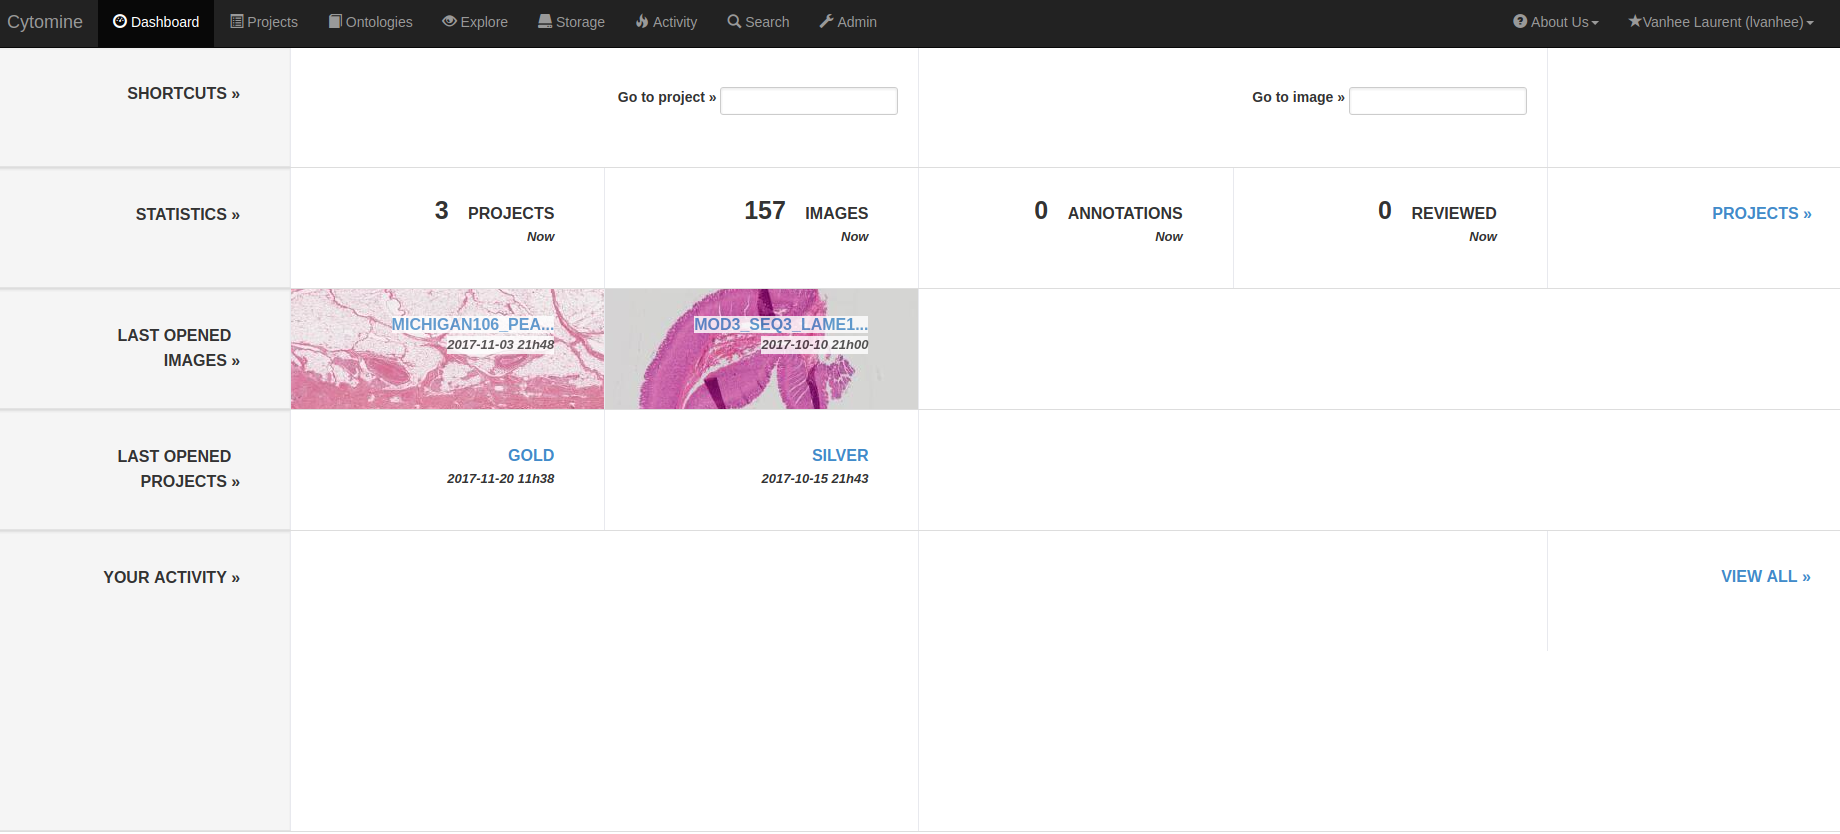
\includegraphics[width=.95\linewidth]{images/cytomine_home.png}
      \caption{Cytomine MOOC home page}
      \end{figure}

The MOOC server is a Cytomine Web Application used for education by the Faculty of Medicine at the University of Liege.
It is used for the HISL0541 (General histology and alternative experimentation methods that do not use animals) course.
This course is organized for students enrolled for a Bachelor in Medicine.
Students have to study tissue samples. (Figure \ref{fig:lame_example})

      \begin{figure}[H]
      \centering
      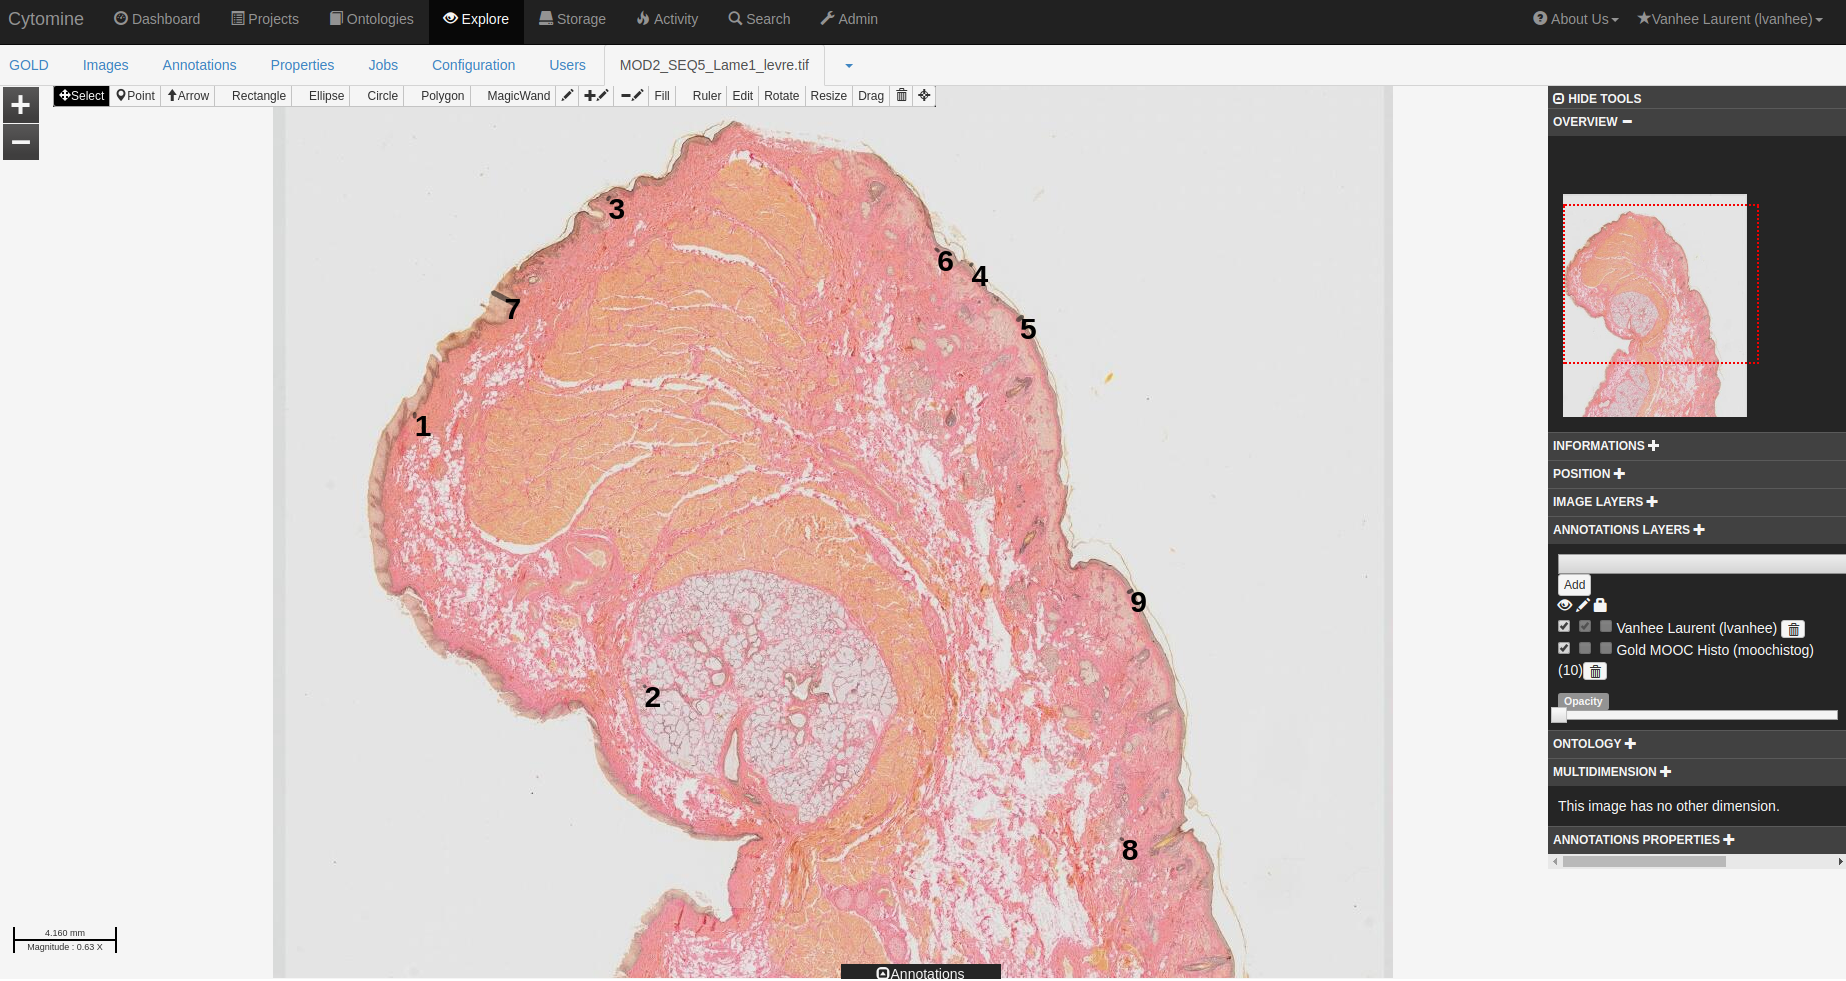
\includegraphics[width=.95\linewidth]{images/lame_cytomine.png}
      \caption{Cytomine MOOC Image example}
      \label{fig:lame_example}
      \end{figure}

Cytomine is a great tool for this particular field because it can be used to store and display high quality images of tissue samples.
It is also easily accessible for the students outside lab sessions as it is available 24 hours a day.
The details of the assignments are given by Ecampus which is communication tool for students and teachers delivered by the University.
The teachers can also use Cytomine to explain certain visual concepts in real-time.
They can also use certain images for exercises by telling students to look for patterns in those images.\\

Since the MOOC is completely integrated to the course, it directly impacts how students learn.
Their exams are often based on what they learned using the tool.
The goal is to see how much of an effect Cytomine has on students.


\section{Teacher Input}

    Opinions on professionals that had the opportunity to work with Cytomine is very important if development were to continue.
    This input seen in ~\cite{hist} comes from the teachers who use Cytomine in the field of Medicine.
    The development of new tools and methods have heavily influenced the ways teachers approach their courses.
    This includes the sharing and consultation of resources online.
    Every year, over 500 students from the Faculty of Medicine at the University of Liege partake in this new learning approach.
    The team working on the courses wanted to extend that knowledge and share it to a wider audience.
    This is where the MOOC server becomes interesting.
    MOOC stands for Massive Open Online Course.
    The courses that use the MOOC encourage democratization of the sharing of knowledge.
    The free access to high quality educational resources is now possible.
    In fact, there are platforms (for example : https//www.fun-mooc.fr) that share multiple MOOCs to encourage this principle.
    The MOOC is used in parallel with traditional courses.
    With the HISL0541 course, the teachers divided the contents into 6 modules.
    The first being a introduction to histology, and the rest a more concerns the vast family of tissue.
    They invite students to explore and observe multiple images.
    They offer two projects (GOLD and SILVER) that people can participate in (not only the students that follow the HISL0541 course).
    At the end, these participants are offered to partake in activities that can give them certificates.
    If the participants succeed with a score of 70\%, they are given a certificates.
    Over 5000 participants that range from young to old, from students to employed workers, and from many different countries have participated in the MOOC.
    Overall most participants seemed very motivated and satisfied with this approach.
    This sharing of knowledge in a interactive and accessible way is great for anyone that have interests in this topic.


\section{General Goals}


    The Main objective is to observe how the students use Cytomine.
    Since Cytomine is still in development, an objective is to make it robust and user friendly.
    This analysis can give some insight on what works well and what doesn't.
    As a follow up, it would be interesting to see the patterns that that can be observed in regards to the user.
    The teachers also provided some information on students that followed the course.
    This includes the grade obtained and all the tests that lead to that final grade.
    With this information, machine learning can be used to analyze these grades and what patterns lead to them.
    This analysis returns statistics in many forms since there is a wide range of variables. (Figure \ref{fig:highlevel})

      \begin{figure}[H]
      \centering
      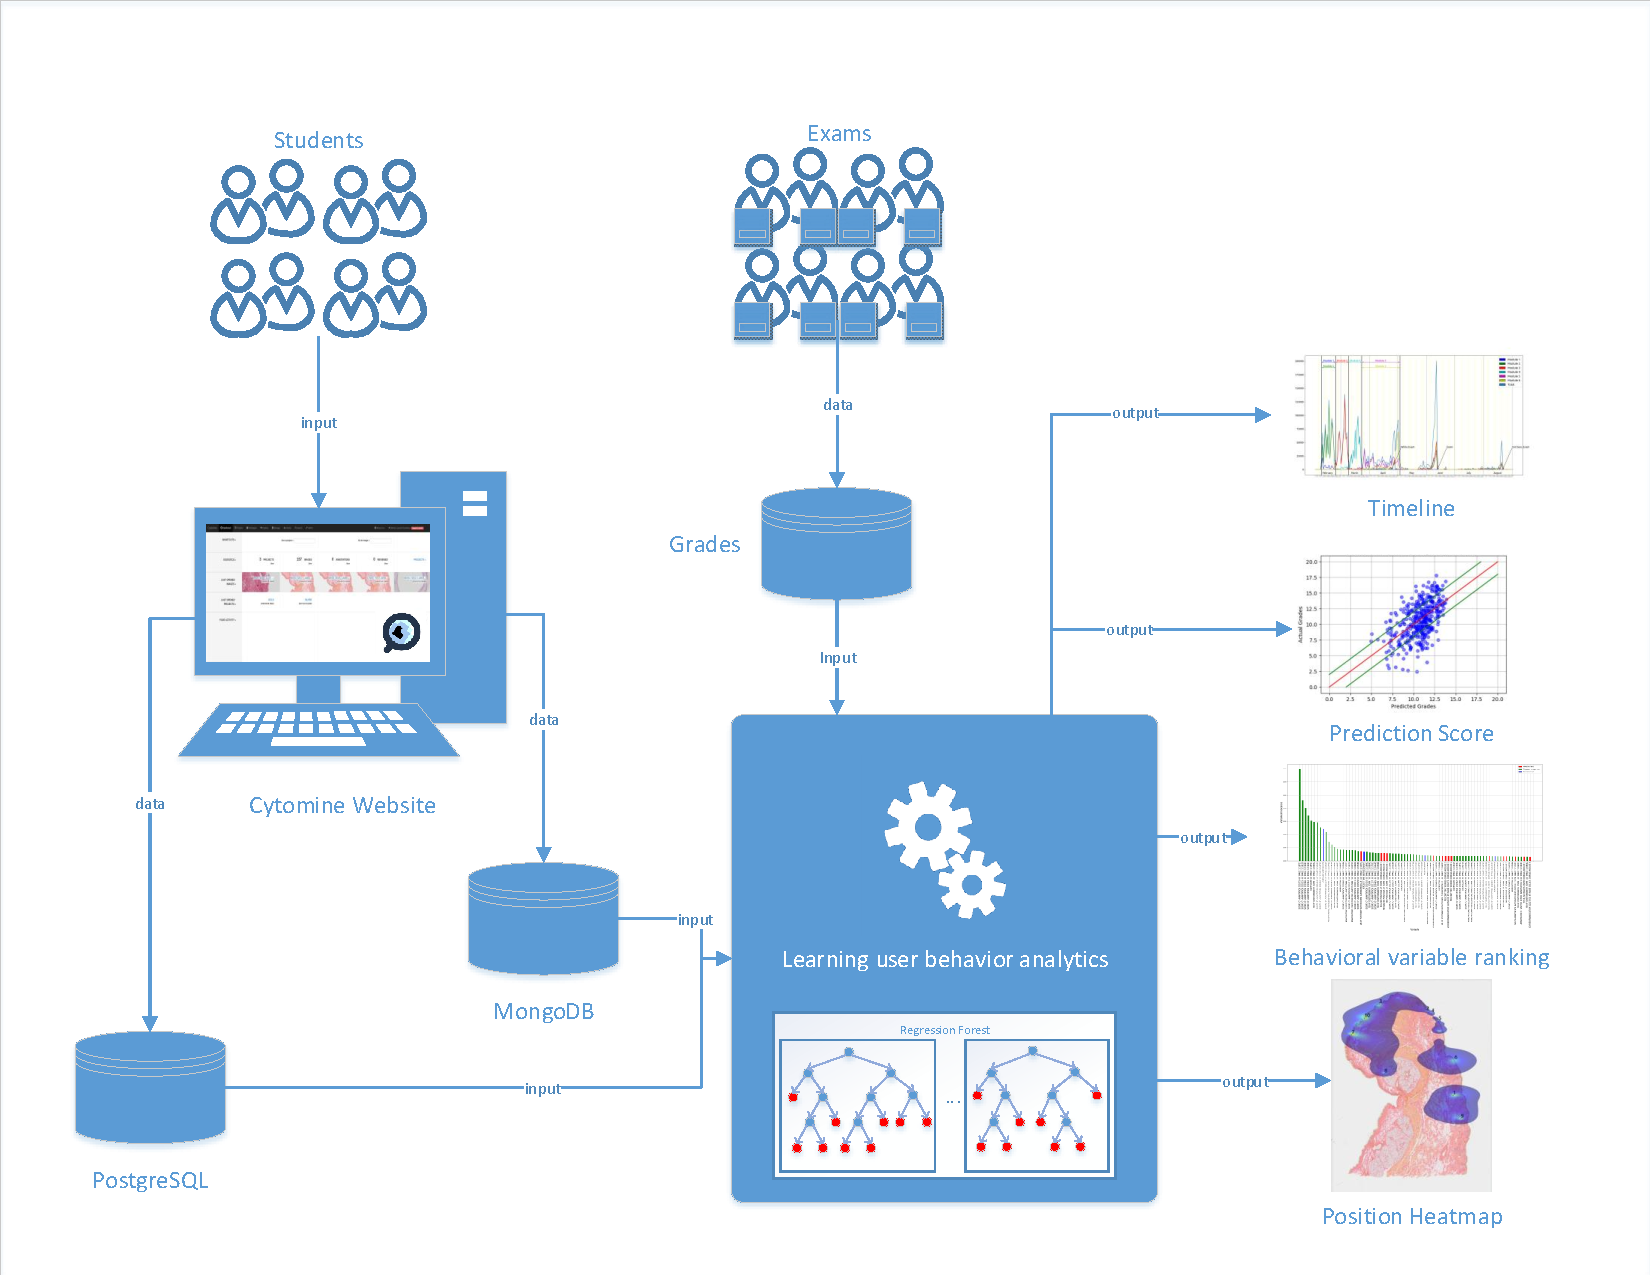
\includegraphics[width=.95\linewidth]{diagrams/highlevel.jpg}
      \caption{High Level View of the Tool}
      \label{fig:highlevel}
      \end{figure}

\section{Previous Studies}

This is not the first attempt to analyze a person's behavior when scanning through cellular images.
~\cite{pathedex}, ~\cite{pathexams}, and ~\cite{pathinterations} all tackle this problem.
~\cite{pathedex} compares image viewing patterns between students and pathologists.
They study high level patterns like the number of fixation points in an image (E.G. positions).
The users are split into two classes based on their diagnostics that were either good or bad.
Finally, they used learning techniques like Markov Chain Monte Carlo to do predictions.

~\cite{pathinterations} focuses more on microscope observations instead of high quality images.
This leads to different patterns compared to the previous study.
Experts were used to create dictionaries of viewing patterns.
Dictionaries of different experts can be merged to form a new dictionary.
This can be used to propose techniques that can automatically identify certain patterns in images.
It can help diagnose conditions like cancer.

~\cite{pathexams} explores viewing patterns in students.
During an exam, they track the students' focus on images with software based  path tracking methods.
In this case, they used a binary classifier.
Either the students passed or failed.
Tree based classifiers were implemented and tested.
Features would also include high level patterns like the number of view steps and average zoom.

These studies are similar in a sense that they analyze user scanning of images and compare it with a performance criteria (E.G rate of detecting cancer).
They also often analyze a set of students and how they behave will scanning images.
The main difference is that in this study, students go through more than one image and regression is used instead of binary classification.
Since they are assessed from their performance as a whole, this analysis cannot be donne image by image.
Since images are often vastly different, information retrieved and studied need to be more general.
In this study, obtaining the data is also much easier.
The students are not subject to specialized tools that track them during their exams.
Data is stored over time in a Server when the user uses the website.
The fact that they are unaware that the data is used for analysis makes the study more compelling.


\chapter{Tools and Methods}

    Cytomine developed with many tools that makes it user friendly ~\cite{cyt}.

    \section{Cytomine Databases}
    % todo ask if allowed to use figures from the Cytomine website
    Data comes in different shapes and forms, therefore different methods are used to store this data.
    The databases included are :
    \begin{itemize}
        \item[\textbullet] \textbf{PostgreSQL} : A object relational database that stores most of the Cytomine information.
        Its functions are to store data and return this data queried by applications.
        This information includes projects, software execution and many other forms of data.
        The Postgis extension was used to store information like annotations and regions of interest.
        \item[\textbullet] \textbf{MongoDB} : A document NoSQL database.
        It's designed for storing and managing semi-structured data.
        It follows the key-value store principle.
        It's particularly useful for information that changes constantly because of its response time.
        MongoDB uses JSON like documents to store this information.
        For Cytomine it is used for user activity which includes user positions and user connections.
        \item[\textbullet] \textbf{File Systems} : Information simply stored in directories and folders.
        The previous database methods cannot handle Images.
        These images that are store with file systems are often very high resolution images.
    \end{itemize}

    This data is retrieved locally by the Cytomine Core Application.
    In order for a user to retrieve this information, a Application programming Interface (API) was implemented.


    \section{Cytomine API}

    The Cytomine API allows for a user to retrieve data from the server.
    It is defined as a REST API.
    It follows an architectural style that defines a set of constraints and properties based on HTTP.
    It defines a predefined set of stateless operations.
    All interactions with the Cytomine Core is done through the REST API.
    This includes communication with the Cytomine Python Client.\\

    The cytomine Python Client is a add-on to Cytomine for easy communication between the user and the server using the Python programming language.
    It includes methods that returns the called information in a more structured like manner.
    Methods to retrieve image and user information were used for this analysis.

    \section{Machine Learning and ExtraTrees}

    Machine learning was used throughout this project as a tool for analyzing user behavior.
    Machine Learning in short are algorithms that make predictions based on previous observations.
    There are many variations of machine learning methods but the two main families include :
    \begin{itemize}
        \item[\textbullet] \textbf{Supervised Learning} : The goal is to match an input with an output.
        The algorithm is given a large amount of input/output pairs for the goal of learning.
        When it is done learning it can be given a input variable that it tries to classify.
        For example, a machine learning algorithm can be given a set of images that contain a dog and a set of images that contain no dog.
        When the algorithm finished learning what rules determine whether or not a dog is in an image, it can be tested with new images.
        The algorithm tries to guess which images contain dogs and which don't.
        The algorithm needs to be tested in order to determine frequency of predictions are correct.
        This methods often requires a large amount of data to work effectively.
        Machine learning can support two types of outputs :
        \begin{itemize}
            \item Classification : Output data is split into different groups.
            Very often data is classified into two groups (for example, whether or not a patient has cancer).
            But data can also be classified into a larger number of groups (for example, classifying drawings of the letters in the alphabet).
            \item Regression : Unlike classification, data cannot be separated into groups.
            Instead the outputs belong in a certain range of values.
            This is used for this analysis tool to predict grades that range from 0 to 20.
        \end{itemize}
        \item[\textbullet] \textbf{Unsupervised Learning} : Unlike supervised learning, unsupervised learning tries to find patterns and correlations in the data.
        Also the data is not labelled therefore supervised learning is not permissible.
        A form of unsupervised learning that is very popular is clustering.
        The goal with clustering is to group different individuals that share similar characteristics.
        A widely used technique used in this analysis is the K-means clustering.
        It uses distances (often Euclidean) to compare individuals.
        The number of distances is determined by K.
        At the start, individuals are placed in random clusters.
        At each step, individuals are moved to the closest cluster.
        There are many ways to define the closest cluster, a common one is the closest center of the cluster to the individual.
        The algorithm ends when the clusters barely change between iterations.
        For this project, it is used to cluster many user positions to draw better scan paths.
    \end{itemize}

    There are many supervised learning techniques that can be used to learn labeled data.
    Methods include K-NN, linear regression, neural networks, and many others.\\

    The focus on this project was to work with regression trees.
    Since the main goal is analysis and not machine learning, regression trees provides much insight into the roots of the results with the feature importance tools it provides.
    When building a tree, the idea at each step is to look for the features that best split the remaining dataset based on the values of the features.
    It uses an impurity measure to determine whether or not to branch further down the tree.
    When the tree is built, an individual's target value is represented by a leaf of a tree.
    It is important to build the tree properly to avoid overfitting and underfitting.\\

    Trees are often not the most accurate of predictors but it is possible to use Ensemble Methods to obtain a better predictive performance.
    Ensemble methods combine multiple different learning algorithms and often work better when working with small datasets.
    The ensemble method subject for this project is the Extremely Randomized Trees (ExtraTrees) as described in ~\cite{extratree}.

    The problem with most tree based methods is the high error rate often due to the high bias and variance.
    This often happens due to overfitting or underfitting.
    Overfitting occurs when the model is too dependent on the data set used for training, when testing on a different set the error would be much higher than anticipated.
    Underfitting is the exact opposite, it occurs when the model is unable to properly train the data often because it is too simple.
    Unlike previous tree based ensemble method, the ExtraTree method selects splits of both features and cut-points partially or totally at random.
    For each node, it is combined with a random choice of a certain number of features, among which the best one is determined.
    Using Ensemble techniques, many trees can be built in parallel.
    Predictions can be made with the ExtraTree Regressor and and the final output becomes a average between the output of all the trees.
    With this randomization, the ExtraTree should be able to reduce the variance more effectively than other weaker randomizing methods.
    It also uses the full learning sample for each tree, thus minimizing bias.
    Overall this handles overfitting very well for most learning samples.
    To avoid underfitting, building the ExtraTree with enough estimators is usually enough.\\


    The following algorithm described in ~\cite{extratree} explains how the splitting is done at a tree node:
\noindent\fbox{%
    \begin{algorithm}[H]
        \caption{Split\_a\_node(S)}
        \SetAlgoLined
        \RestyleAlgo{boxruled}
        \KwIn{the local learning subset $S$ corresponding to the node needed to be split}
        \KwOut{a split $[ \, a < a_c ] \, $ or nothing}
        \eIf{\textbf{Stop\_split($S$)} == True}
            {Return nothing\;}
            {--Select $K$ features $ \{ a_1, ..., a_K  \} $ among non constant candidate features in $S$\;
             --Draw $K$ splits $ \{ s_1, ..., s_K  \} $ with $s_i$ = \textbf{Pick\_a\_random\_split($S$, $a_i$)}, $\forall i \in [ \, 1 , K ] \, $\;
             --Return a split $s_*$ such that Score($s_*$, $S$) = $max_{i = 1,...,k}$Score($s_i$, $S$)\;}

    \end{algorithm}
} \\
\noindent\fbox{
    \begin{algorithm}[H]
        \caption{Pick\_a\_random\_split($S$, $a$)}
        \SetAlgoLined
        \RestyleAlgo{boxruled}
        \KwIn{a subset $S$ and a feature $a$}
        \KwOut{a split}
        --$a^S_{max}$ and $a^S_{min}$ the maximal and minimal values of a in $S$ \;
        --Draw random cut-point $a_c$ uniformly in $[ \, a^S_{min}, a^S_{max} ] \, $\;
        --Return a split $[ \, a < a_c ] \, $\;
    \end{algorithm}
} \\
\noindent\fbox{
    \begin{algorithm}[H]
        \caption{Stop\_split(S)}
        \SetAlgoLined
        \RestyleAlgo{boxruled}
        \KwIn{a subset $S$}
        \KwOut{a boolean}
        \If{$|S| < n_{min}$}
           {Return True\;}
        \If{all features constant}
           {Return True\;}
        \eIf{Output constant}
            {Return True\;}
            {return False\;}
    \end{algorithm}
}
    When picking a random split, a feature $a$ contains values ranging from $a_{min}^S$ to $a_{max}^S$.
    A split belonging to this range is then chosen at random.
    This is done $K$ times and the best split is chosen for this node based on the scores of the splits.
    In regression, a score is measured by calculating the amount of output variance reduction.
    With $S_l$ and $S_r$ the two subsets of from $S$ corresponding to the two outcomes of a split $s$.
    The score is defined as :
    $$Score_R(s,S) = \dfrac{var \{ y | S \}   - \dfrac{|S_l|}{|S|} var \{  y | S_l \}  - \dfrac{|S_r|}{|S|} var \{  y | S_r \} }{var \{  y | S \} } $$
    with $var \{  y | S \} $ the variance of the output $y$ in the sample $S$.

    \section{Three Separate Components}
    	Since there is a vast amount of data, most operations require a good amount of time to complete.
    	Therefore, the data analysis tool is divided into three components :
        \begin{itemize}
        \item[\textbullet] Data Acquisition (download\_data.py).
        \item[\textbullet] Data Manipulation (data\_manager.py).
        \item[\textbullet] Data Learning (data\_learning.py).
        \end{itemize}

        The code is available at Github (https://github.com/lvanhee42/Master-Thesis).

		\subsection{Data Acquisition}

			During the 2016-2017 Academic year, Cytomine tracked and stored user information on the MOOC server.
			To obtain all this information, Cytomine is accessible by a REST API. To ease the access to the server, Cytomine developed a Python Client that was used for the acquisition of relevant information.
			With administrator rights, a user can get a hold of all if not most of the data stored on the SQL and MongoDB databases.

          There are currently a total of two projects called GOLD and SILVER that students could participate in.
          To start of, each project contains a set of images and a set of students that have signed up.

          \begin{center}
          \begin{tabular}{| l | c | c |}
          \hline
           & Number of students & Number of images \\ \hline
           GOLD & 395 & 78 \\ \hline
           SILVER & 85 & 75 \\
          \hline
          \end{tabular}
          \end{center}

		  Both projects have their own objectives but GOLD is more complete and thorough.
		  unlike the SILVER project, the students were tested and graded on the course that was given to them but also the content of the project.

          To analyze user behavior, it is necessary to fetch data that is relevant, this includes (as shown in Figure \ref{fig:data}):

          \begin{itemize}
          \item[\textbullet] \textbf{Resized images :}\newline

          The images stored on Cytomine are in fact very large.
          For the analysis, a copy of the images will be useful.
          Many operations in the Data Manipulation component rely on the image resolution when it comes to complexity.
          It is important that the image is big enough to be viewable while small enough so that the operations done in a reasonable amount of time.
          The image downloaded is therefore rescaled to a maximum width and height of 1024 pixels.\\
          \item[\textbullet] \textbf{Reference Annotations :}\newline

          When observing images, students are usually given guidelines in forms of image annotations.
          These annotations are zones in the image that contain information that students can learn from.
          These annotations are given a number.
          Annotations from the same image have a different numbers.
          This represents the recommended order the user can traverse the image.
          In this study, only the geometrical center of the annotation is kept.
          In most cases, this loss of information should have no impact because the size of the zones are usually a couple pixels wide when put in the resized image.
          Reference annotations are drawn similarly to the example in Figure \ref{fig:annnn} that are indicated by numbers.\\
            \begin{figure}[H]
              \centering
              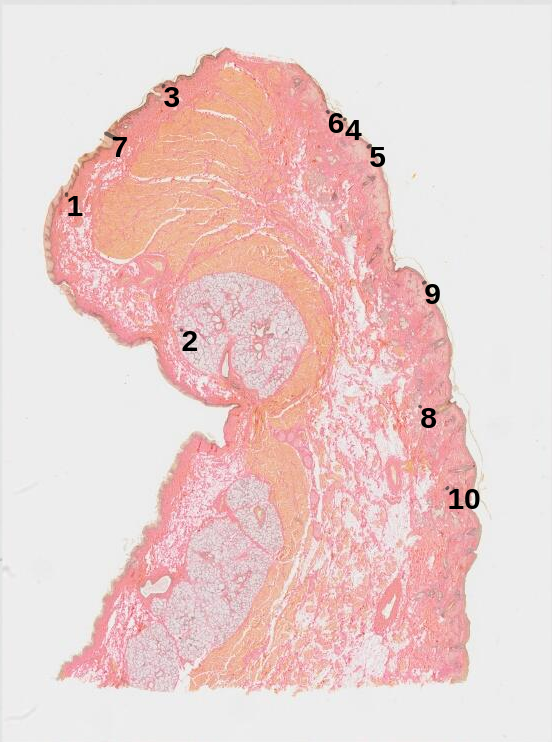
\includegraphics[width=.4\linewidth]{images/annotations.png}
              \caption{Example of Reference annotations}
              \label{fig:annnn}
            \end{figure}
		\item[\textbullet]  \textbf{User Annotations :}\newline

        Teachers can set annotations as guidelines, but normal users can also create annotations.
        If a student user notices something interesting on a patch of an image, that student can annotate it.
        Later, that student could for example approach a teacher with a question and use the annotation as a reference.
        Unfortunately, there are currently no user annotations.
        This will be discussed in section \ref{Discussion}.\\

        \item[\textbullet]  \textbf{User Positions :}\newline

         This is the most important information.
         A position is what the user sees at a current time stamp.
         positions are defined by its center, four corners, time recorded, and zoom.
         Unlike common gaze data, positions here are not collected from the tracking of eye movements, they are based on what the user sees on the screen.
         positions are saved on a regular basis when a user observes an image.
         More precisely positions are saved :
         \begin{itemize}
         	\item[\textbullet] Every 5 seconds.
            \item[\textbullet] When the user switches zooms.
            \item[\textbullet] After the user finishes a movement on the image.
         \end{itemize}
         Due to how frequently positions are recorded, this information comes in large quantity.
         Unfortunately, with all browsers (E.G. Google Chrome and Firefox) positions are still recorded when the page is minimized or tabbed out.
         This means that users can browse some unrelated website or even read course's Syllabus while positions are still recorded on Cytomine.
         The issue is that it is hard to determine whether or not a position is considered invalid because the user was not focused on it during the time.
         An idea that was attempted was after a certain amount of positions with the same coordinates, is to remove the following positions with that coordinate.
         Unfortunately, it requires the setting of a threshold.
         This threshold would be arbitrary.
         After some attempts, this loss of information became a detriment to the Machine Learning and the results were worse.
         Therefore, the idea has been put on hold.
         A visualisation of the different zooms can be shown in Figure \ref{fig:zooms}.\\


         \begin{figure}[H]
            \centering
            \begin{subfigure}[b]{0.3\textwidth}
            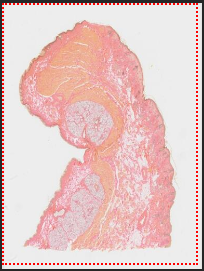
\includegraphics[width=\textwidth]{images/zooms1.png}
            \caption{Zooms 1 to 3}
            \end{subfigure}
            \begin{subfigure}[b]{0.3\textwidth}
            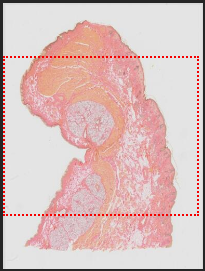
\includegraphics[width=\textwidth]{images/zooms2.png}
            \caption{Zoom 4}
            \end{subfigure}
            \begin{subfigure}[b]{0.3\textwidth}
            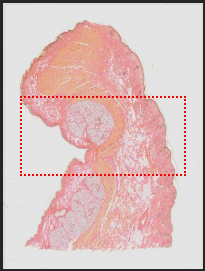
\includegraphics[width=\textwidth]{images/zooms3.png}
            \caption{Zoom 5}
            \end{subfigure}

            \begin{subfigure}[b]{0.3\textwidth}
            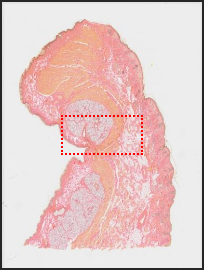
\includegraphics[width=\textwidth]{images/zooms4.png}
            \caption{Zoom 6}
            \end{subfigure}
            \begin{subfigure}[b]{0.3\textwidth}
            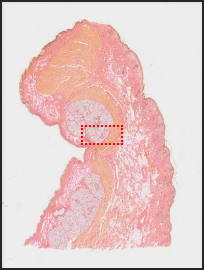
\includegraphics[width=\textwidth]{images/zooms5.png}
            \caption{Zoom 7}
            \end{subfigure}
            \begin{subfigure}[b]{0.3\textwidth}
            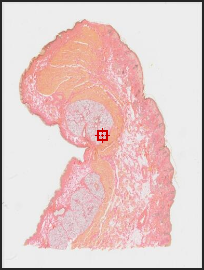
\includegraphics[width=\textwidth]{images/zooms6.png}
            \caption{Zooms 8 to 10}
            \end{subfigure}
            \caption{Figure of different zooms on image 1217722}\label{fig:zooms}
        \end{figure}

        \item[\textbullet] \textbf{Annotations Actions :}\newline

        Annotations are clickable.
        When clicked, a toolbox appears giving more information on the annotation.
        This action is also stored on the server.
        For the data recorded in 2017, an annotation action only contains a time stamp.
        It is only in later versions of Cytomine that the reference annotation identifiers were tracked with the annotation actions.
        In the case where the referenced annotation is unknown, it will be guessed based on positions that appear at the same time.

         \end{itemize}

       \begin{figure}[H]
        \centering
         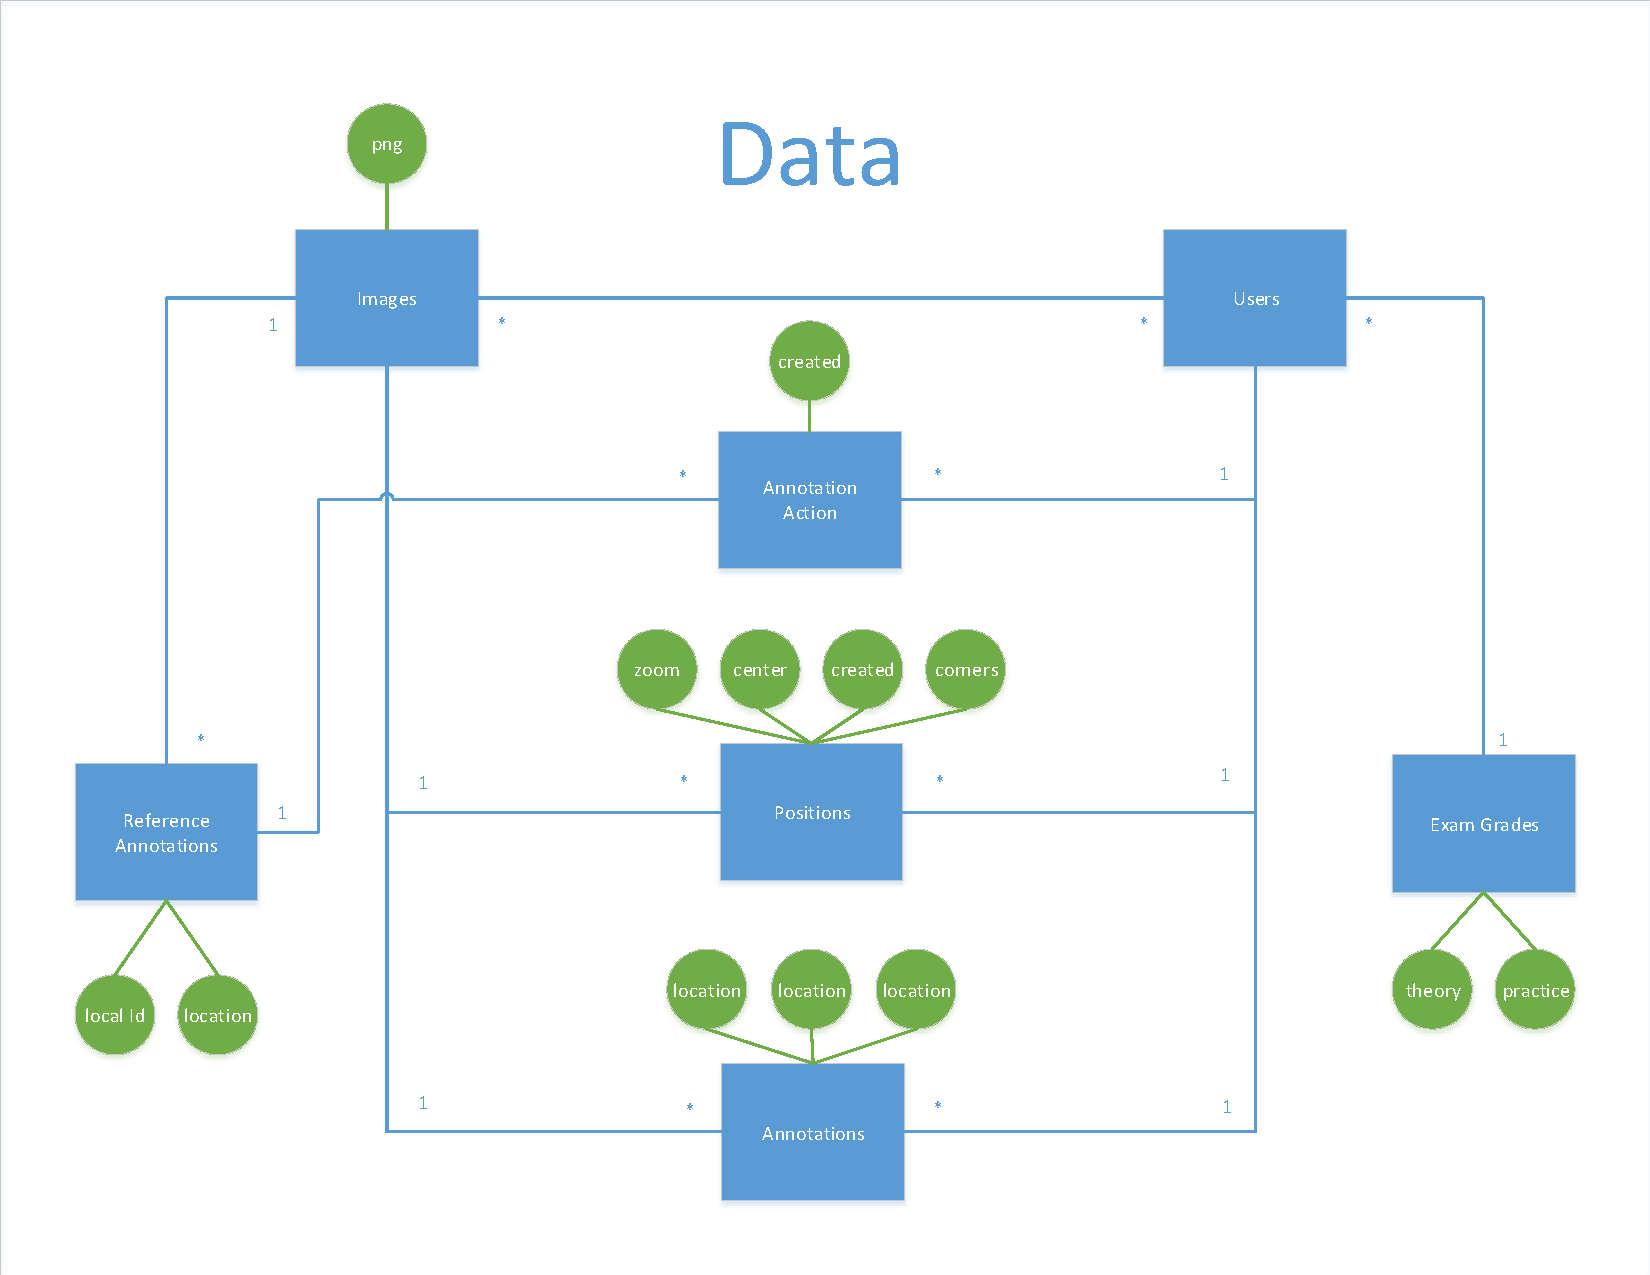
\includegraphics[width=.9\linewidth]{diagrams/dataDiagram.pdf}
         \caption{Data and their relations}
         \label{fig:data}
       \end{figure}


		All this information needs to be downloaded which, unfortunately can take up to 8 hours using the API while putting stress on the MOOC server.
		After some interruptions to the service, it was necessary to install the MOOC locally with backups of the original. \newline


        For both projects, an excel file containing user information not found on Cytomine was given.
        For the SILVER project, this only included basic information that were irrelevant to the analysis (names, emails, etc..).
        Meanwhile for the GOLD project, the University of Liege students had to partake in multiple graded assignments.
        The excel file given for the GOLD students therefore contained grades for numerous activities.
        These grades will be useful in order to understand some aspects of the user behavior on Cytomine. \newline

        To use this component, one can call the \textit{download\_data} script.
        This script comes with some needed parameters (the order must be respected):
        \begin{itemize}
            \item[\textbullet] \textbf{<project\_name>} : The name of the project (For example, gold or silver).
            For this component, it is also the name of the root directory that will contain all the data that will be downloaded.
            When running this component multiple times with the same name, the data will be overwritten each time.
            \item[\textbullet] \textbf{<project\_id>} : The Cytomine identifier of the project to run the script on.
            The reason to have both the name and identifier is to be able to have multiple versions of the same project stored in different directories.
            \item[\textbullet] \textbf{<user\_data>} : Contains the address to a csv file containing a list of users with information that cannot be retrieved from Cytomine.
            The file is structured similarly to the format described in section \ref{experiments}.
            The column named 'CYTOMINE ID' is necessary.
            It contains the user Cytomine identifiers that need to be valid.
            Otherwise, the file contains data which includes grades and other basic user information.
            \item[\textbullet] \textbf{<ref\_user\_id>} : This field contains the identifier of the user who set the reference annotations.
        \end{itemize}
        Otherwise, the next fields are optional and can be added in any order after the mandatory parameters.
        \begin{itemize}
            \item[\textbullet] \textbf{-H <host>} : The <host> field contains the Cytomine MOOC host address.
            \item[\textbullet] \textbf{-PR <key>} : The <key> field contains the Cytomine user private key.
            \item[\textbullet] \textbf{-PU <key>} : The <key> field contains the Cytomine user public key.
            To successfully gain access to the Cytomine website, both the public and private key need to be correct.
            These two parameters are optional because there is a public/private key pair pre-coded into the component.
            \item[\textbullet] \textbf{-I <images>} : The <images> field contains the address to a csv file containing a list of Cytomine image identifiers.
            Each row of the file contains one image identifier.
            This parameter is optional since it is possible to fetch all the image identifiers belonging to a project with the API.
            It is used if the user wants to use the component on a subset of images.
            \item[\textbullet] \textbf{-U <users>} : The <users> field contains the address to a csv file containing a list of Cytomine user identifiers.
            Each row of the file contains one user identifier.
            This follows the same principles than the images.
            \item[\textbullet] \textbf{-M <modules>} : The <modules> field contains the address to a csv file containing a list of modules associated to the course.
            Each row of the file contains one module.
            It's formatted as follows :\newline

              \begin{tabular}{| c | c | c | c | c | c | c | c |}
              \hline
              \tiny{Module Id} & \tiny{Start Date} & \tiny{End Date} & \tiny{Image 1} & \tiny{Type 1} & \tiny{...} & \tiny{Image n} & \tiny{Type n}\\ \hline
              \tiny{1} & \tiny{dd/mm/yyyy} & \tiny{dd/mm/yyyy} & \tiny{$id_1$} & \tiny{T} & \tiny{...} & \tiny{$id_{n1}$} & \tiny{L}\\ \hline
              \tiny{...} & & & & & & & \\ \hline
              \tiny{m} & \tiny{dd/mm/yyyy} & \tiny{dd/mm/yyyy} & \tiny{$id_1$} & \tiny{E} & \tiny{...} & \tiny{$id_{n2}$} & \tiny{B}\\ \hline
              \end{tabular}\newline

            For the types, T represents the tutorials, L represents learning images, E represents exercise images, and B represents supplements.
            Each module does not necessarily have the same number of images associated to it.
        \end{itemize}


        The project has a dedicated directory to store all this information, usually in a csv format.
        For each data type, image, and user triplet, there is a dedicated file containing this information.
        In conclusion, the following diagram explains the role of this component (Figure \ref{fig:comp1}).

       \begin{figure}[H]
        \centering
         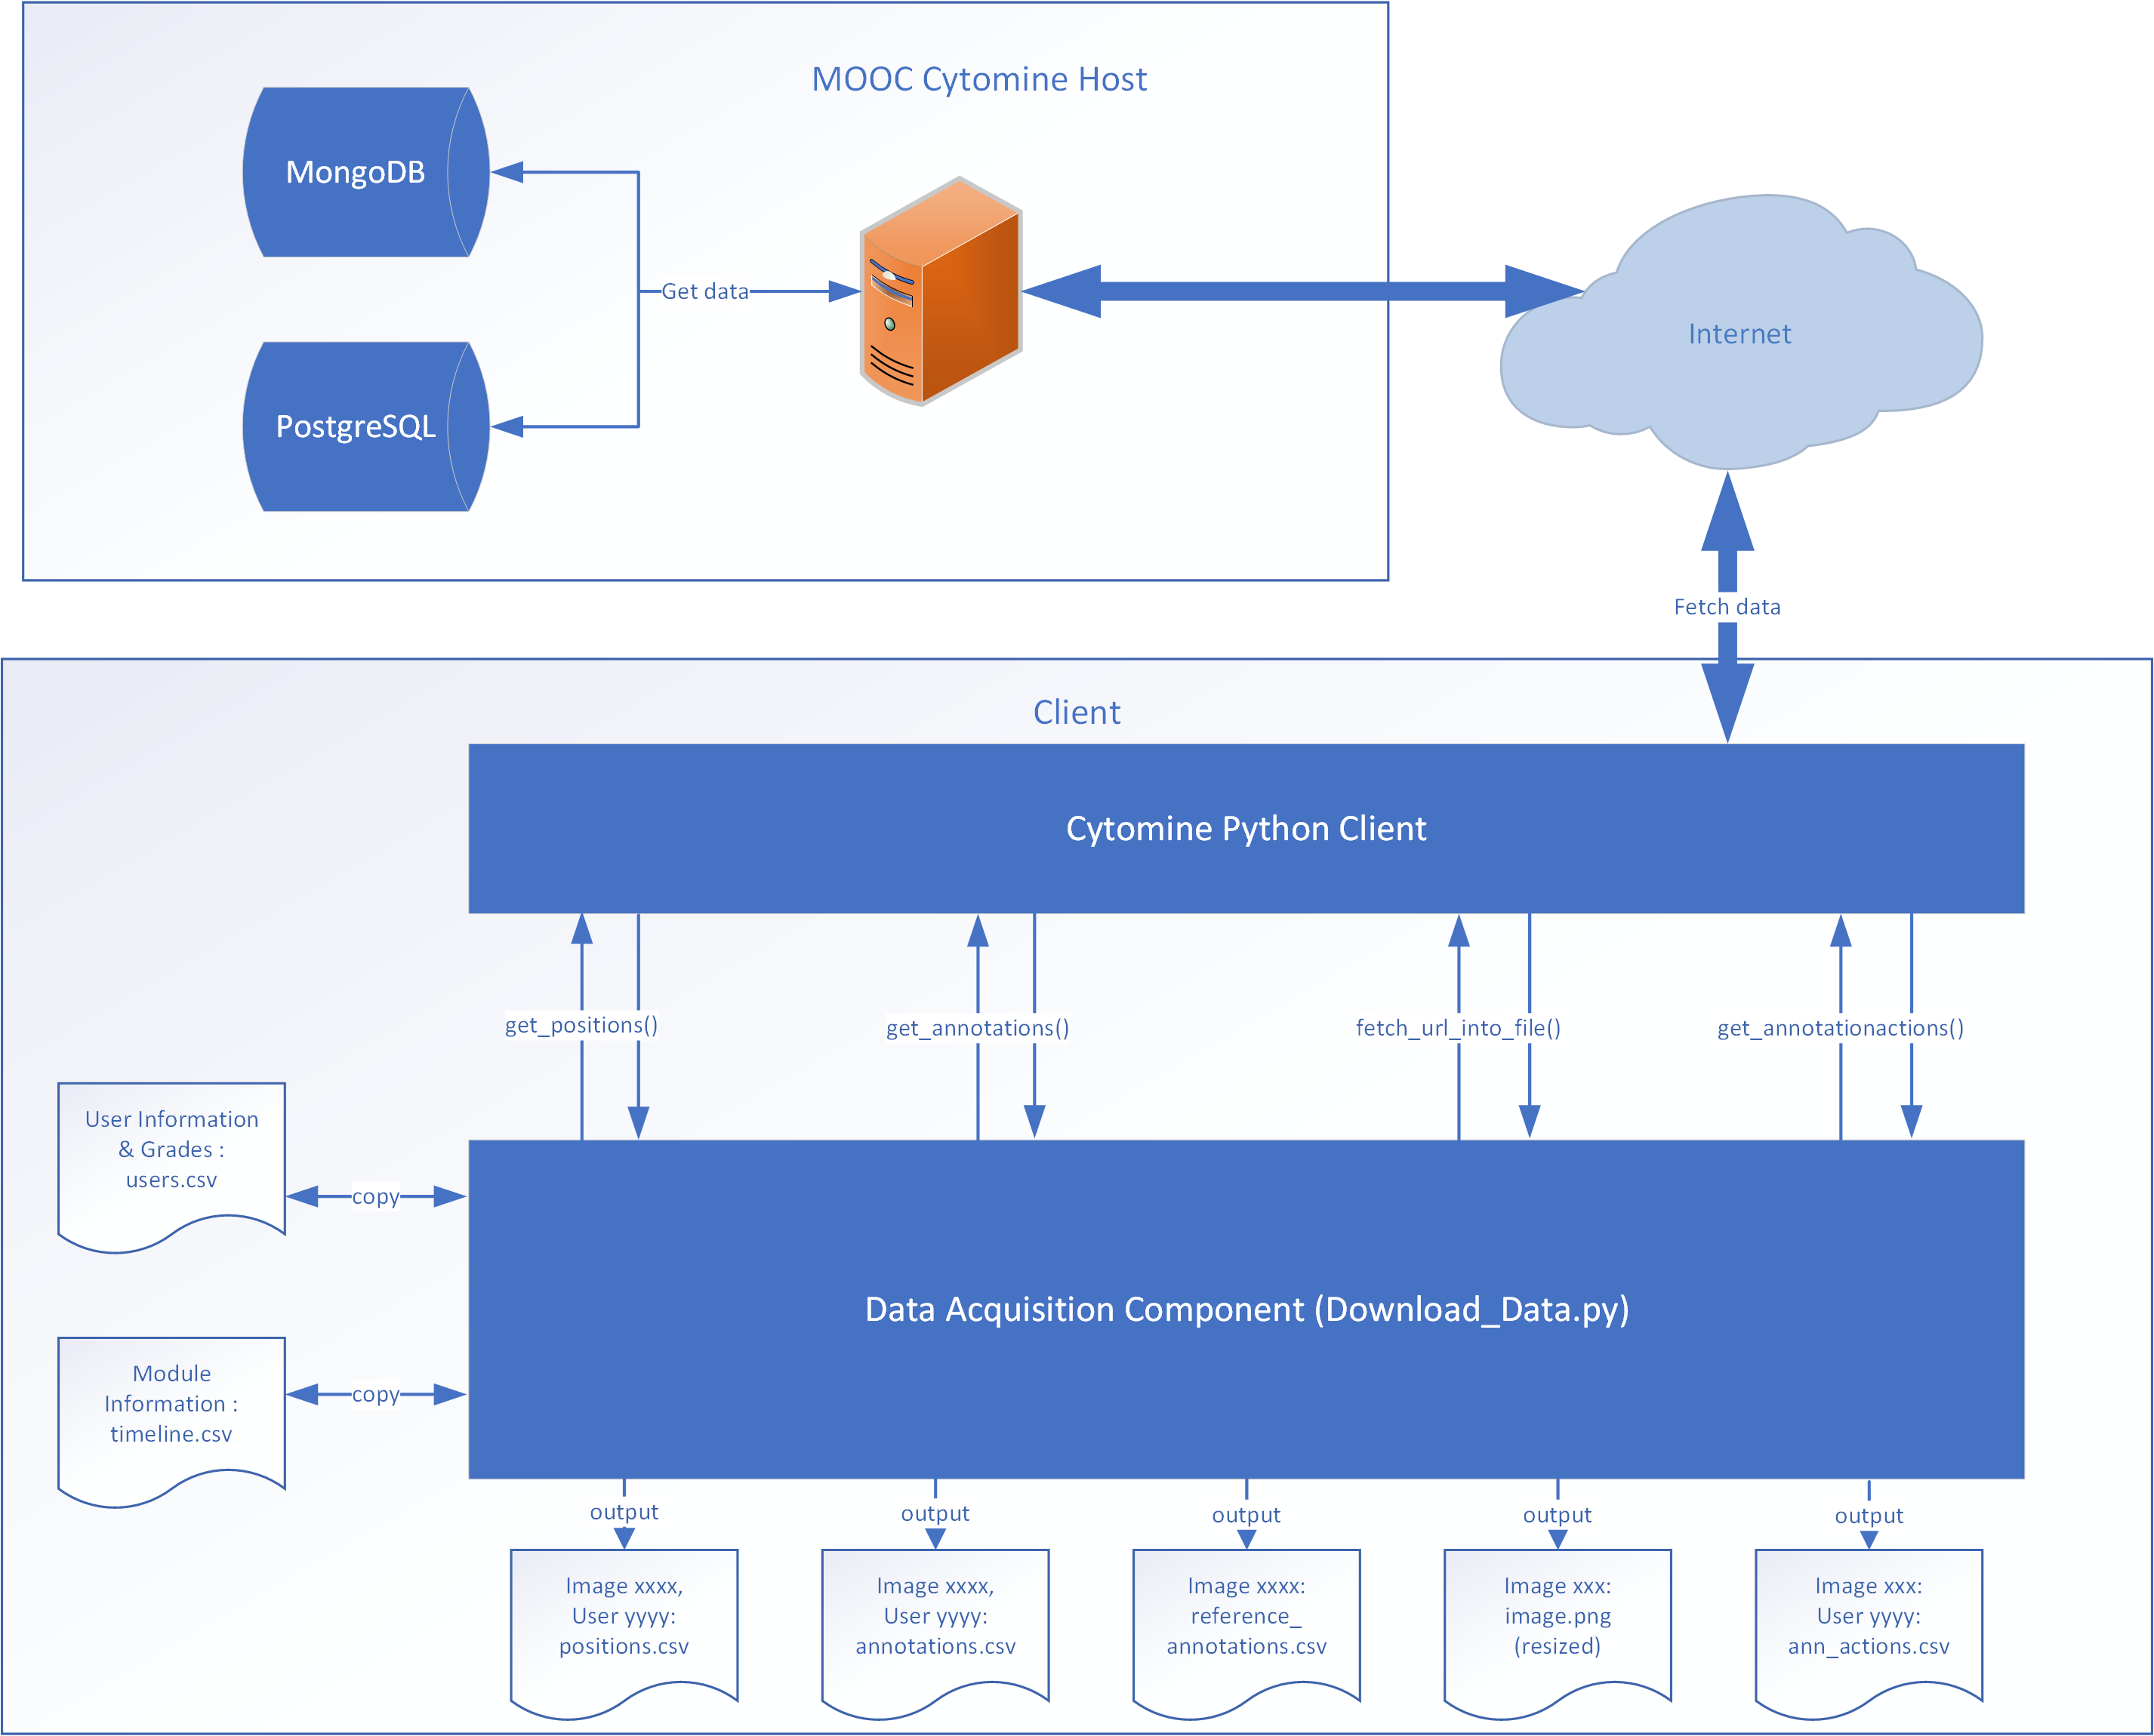
\includegraphics[width=.6\linewidth]{diagrams/module1.png}
         \caption{Data Acquisition Component}
         \label{fig:comp1}
       \end{figure}

        These files will be opened and read by the Data Manipulation Component for generating statistics and ways to represent data visually.
        These files are organized in directories.
        This component, builds an underlying structure that will be used and manipulated by the other components. (Figure \ref{fig:struct})

       \begin{figure}[H]
        \centering
         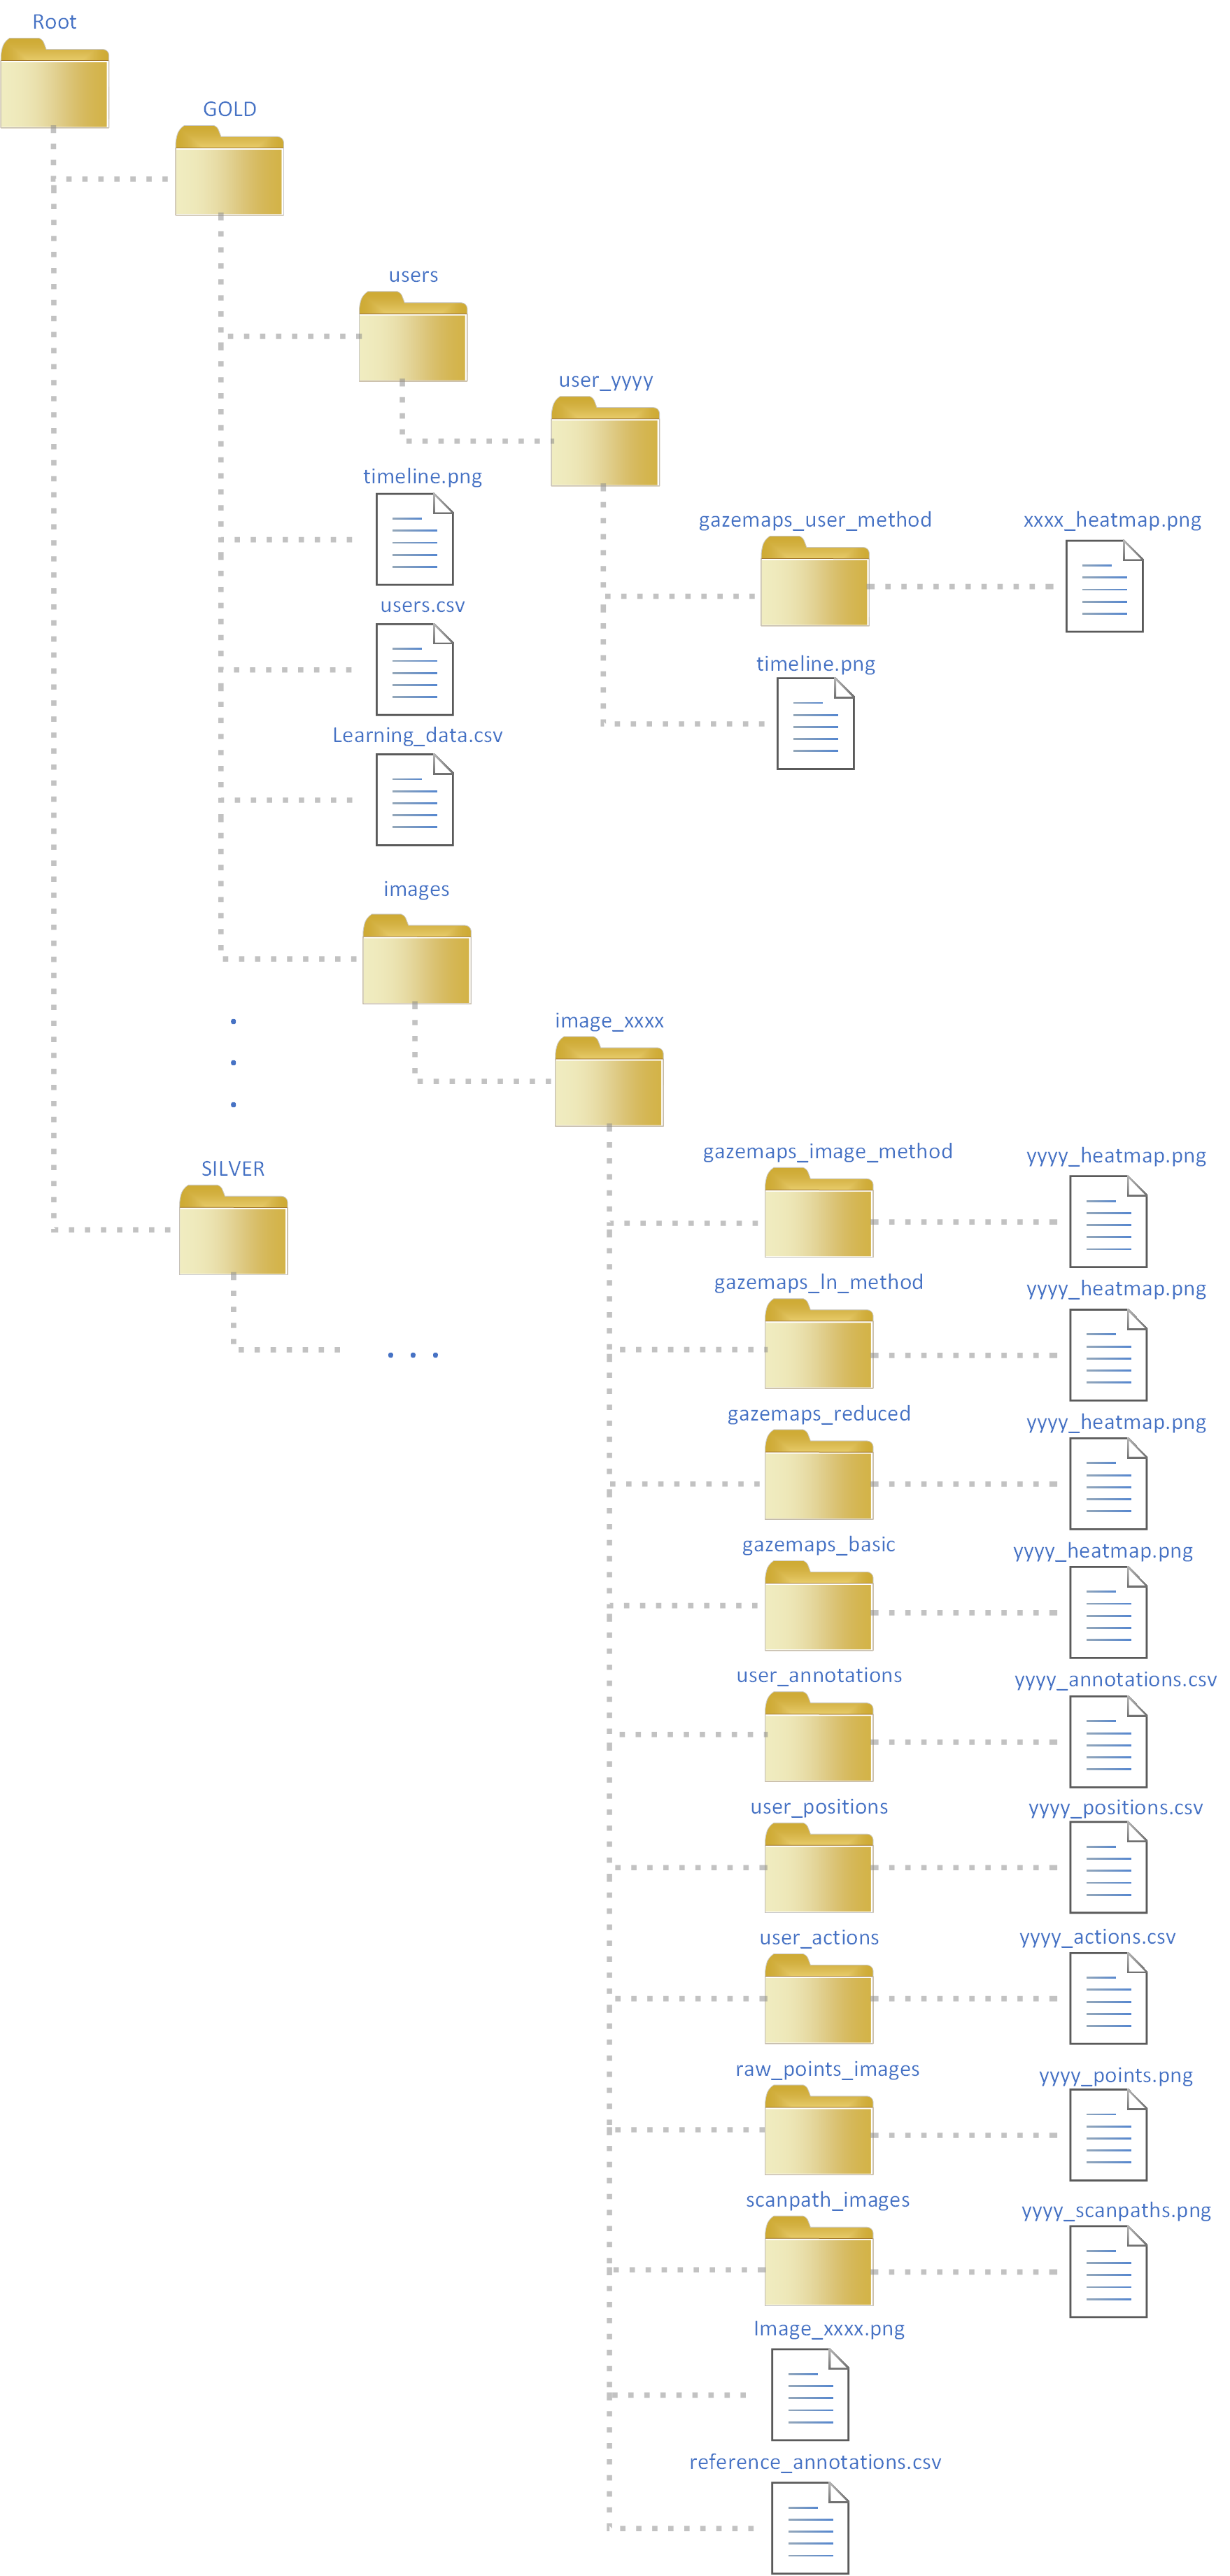
\includegraphics[width=.6\linewidth]{diagrams/directories.png}
         \caption{Directory and File Structure}
         \label{fig:struct}
       \end{figure}

	\subsection{Data Manipulation}

    This component is used to interpret the data that's in its most basic form.
    It has multiple outputs based on the parameters set.
    Since it is important to obtain information as a whole on the data set, the component is divided into two main parts:
    \begin{itemize}
        \item[\textbullet] \textbf{Loading data to Memory:} The positions, the annotations, the actions, and the image information data are all loaded to memory.
        \item[\textbullet] \textbf{Data Handling :} Calling numerous methods that extracts important information.
    \end{itemize}

    This component knows and uses the file directory structure.
    This allows it to find the files necessary to do the analysis.
    An object oriented approach was used in order to handle this information.
    In fact, there are multiple classes:

    \begin{itemize}
        \item[\textbullet] \textbf{Data\_Manager :} This class defines an object that will coordinate between the other classes in order to obtain the valuable information necessary.
        \item[\textbullet] \textbf{Image\_Data :} This class defines objects that will contain references to information on a specific image.
        It also comes with operations associated to said image.
        \item[\textbullet] \textbf{User\_Data :} This class defines objects that will contain references to information on a specific user.
        Similarly, to Image\_Data, it comes with numerous operations.
        \item[\textbullet] \textbf{Module\_Data :} This class defines objects that will contain references to information on a specific module.
        Modules are predefined by the teachers as a set of objectives within a certain timeframe.
        There is a subset of images that are associated to a module.
        It therefore contains references to users and images and it also comes with its own operations.
    \end{itemize}

    These instances contain references to richer information.
    This information is handled using dictionaries for fast and easy access.
    For the set of positions associated to a user and image pair, the dictionary contains these key and value pairs:
    \begin{itemize}
        \item[\textbullet] \textbf{'x' :} Array of X coordinates for all the positions.
        \item[\textbullet] \textbf{'y' :} Array of Y coordinates for all the positions.
        \item[\textbullet] \textbf{'dur':} Array of the duration for all the positions.
        \item[\textbullet] \textbf{'timestamp':} Array of the exact time the positions have been recorded for each position.
        \item[\textbullet] \textbf{'zoom' :} Array of the zoom values for each position (1 to 10)
        \item[\textbullet] \textbf{'corners'} : Array containing the four corners for each position.
        The four corners are stored as an array with 4 values.
        These values contain a pair for the X and Y coordinates.
    \end{itemize}

    It is noted that the positions are sorted in regards to the timestamp value.
    This prevents many problems and makes specific operations much easier.
    The dictionary follows a similar structure for annotations that are either associated to an image and user pair (user annotation) or just an image (reference annotation):
    \begin{itemize}
        \item[\textbullet] \textbf{'x' :} Array of X coordinates for all the annotations.
        \item[\textbullet] \textbf{'y' :} Array of Y coordinates for all the annotations.
        \item[\textbullet] \textbf{'id' :} Array of the identifiers for all the annotations.
        \item[\textbullet] \textbf{'localId' :} Array of the local identifiers for all the annotations.
        Used for reference annotations.
        This property represents the annotation number shown on the images but also the recommended order of passage for these annotations
        \item[\textbullet] \textbf{'type' :} Array of the type for all annotations.
        This is either a point or a polygon.
    \end{itemize}

    There are much fewer annotations then there are positions.
    Finally there are also annotation actions for image and user pairs:
    \begin{itemize}
        \item[\textbullet] \textbf{'id' :} Array of the identifiers of the concerned annotations for all the annotation actions.
        \item[\textbullet] \textbf{'action' :} Array of the action carried out for all annotation actions.
        The value is always 'select'.
        \item[\textbullet] \textbf{'timestamp' :} Array of the time the annotation action was carried out.
    \end{itemize}
    It is important to note that during the period of January 2017 to September 2017, annotation actions were collected but they did not specify which annotation the action was related to.
    To determine that the component guesses the annotation.
    The component finds the position with the closest timestamp and guesses the annotation closest to that position.
    It's not perfect but it guesses the most likely annotation since at most zooms the user can only see one annotation.\\


    This data is referenced by the proper Image\_Data and User\_Data objects for easy access.
    When loading all this data into memory, extra operations have been carried out.
    The most notable being generating the gaussian surface for each zoom associated to each image.
    This uses a 2 Dimensional Gaussian distribution function.
    The Gaussian plane respects the dimensions of the positions associated to that zoom.
    This allows to better represent a position by not just taking into account the center and corners but the entirety of the field of view of the person.
    The goal is to give more importance to the center pixels of a position over the pixels near the edge.
    This will be very important when deriving statistics generating heatmaps.

    When generating the gaussian with a height of $h$ and a width of $w$.
    The standard deviation set for the height and width are $s_h = \dfrac{h}{6}$ and $s_w = \dfrac{w}{6}$.
    $h_0 = \dfrac{h}{2}$ and $w_0 = \dfrac{w}{2}$ are the center coordinates of the surface.
    $coef$ is a coefficient based on the zoom.
    The coefficient is a value from 0 to 1, the higher the zoom the higher the coefficient with $coef = \dfrac{zoom}{max\_zoom}$.
    The equation is :

        \[P(i,j) = \exp(\dfrac{-1}{2}*(\dfrac{(i - h_0)^2}{s_h^2} + \dfrac{(j - w_0)^2}{s_w^2})) * coef \]

    With $i \in [0, h]$ and $j \in [0, w]$.

    With the standard deviation set, 99 percent of the gaussian distribution is in the surface.
    Therefore when calculating the center point, there is an output close to 1.
    Likewise, when calculating a point near the edge, there is an output close to 0.
    An interesting idea that was not implemented was to replace $coef$ with $\dfrac{1}{2\pi*s_h*s_w}$.
    With that, the integral of all the Gaussian surfaces would be equal to 1.
    The problem with this method is with each zoom level, the height and the width halves in size.
    The surface would be four times as small.
    Therefore, from zoom 1 to 10 there is a factor of $4^{10}$ or about a million.
    The difference in values between zooms would be too extreme.
    This is why a more linear coefficient is used so that Heatmaps are observable.
    In the end, the idea is that the human attention is more focused on the center.
    Therefore a Gaussian distribution is ideal for this particular problem.
    In the following example is shown the Gaussian distribution for a surface with a length and width of 100, and a coefficient of 1. (Figure \ref{fig:gaus22})

    \begin{figure}[H]
      \centering
      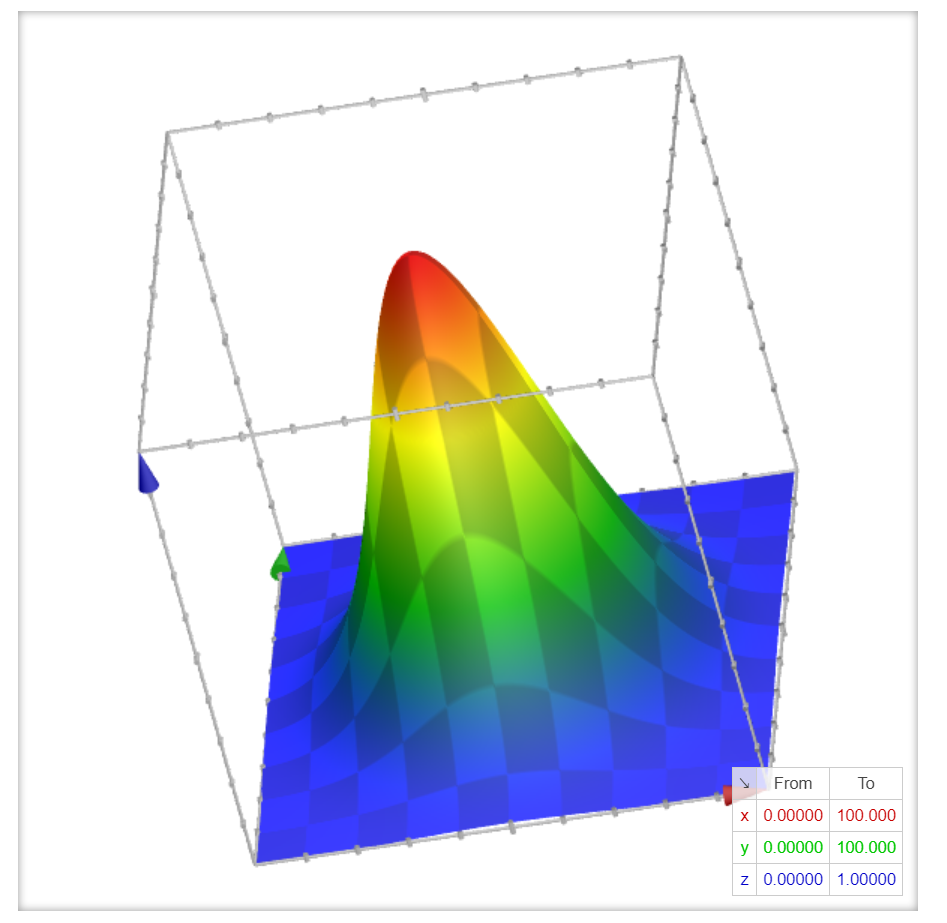
\includegraphics[width=.45\linewidth]{plots/gaussian2D.png}
      \caption{Gaussian Distribution Example}
      \label{fig:gaus22}
    \end{figure}

    Of course, because the work is done on images, there is a limited resolution and the Gaussian is not as smooth.
    This is because each pixel is a point and a point has the value set by the formula.
    \newline

    Once all all this information is stored in memory.
    it is possible to call numerous tasks to analyze the data and draw statistics.
    This component used two libraries :
    \begin{itemize}
        \item[\textbullet] \textbf{PyGazeAnalyser} ~\cite{pygaze} : This open-source library implemented by PyGaze draws statistics about Gaze data.
        This data is often in form of figures.
        In this implementation, it calculates the Gaussian arrays for each zoom and draws the visualisation figures (Gazemap, scan paths, raw points).
        Unfortunately, PyGazeAnalyzer in its current state was not perfectly suitable with the data retrieved from Cytomine.
        It generated heatmaps but did not allow the regularisation for example.
        It also was not compatible with different levels of zoom.
        In fact, this library is more suitable for gaze data that comes directly from capturing eye movements.
        The code was forked and tweaked to handle these changes.
        \item[\textbullet] \textbf{scikit-learn} ~\cite{scikit-learn} : This library implements many learning techniques.
        For this component, the K-Fold clustering method has been implemented in order to group up positions that are close in regards to space and time.
    \end{itemize}

    With these libraries the all the outputs possible include :

    \begin{itemize}
        \item[\textbullet] \textbf{Output a Feature File :} Students are analyzed individually in regards to the images they visited.
        A set of features is then extracted in regards to their behavior.
        (see \ref{Data_Set} for more information on the contents and structure of the file)
        \item[\textbullet] \textbf{Output activity over time figures (Timeline) :} These figure represents the activity over time of a set of students or simply an individual in regards to different modules.
        It gives a good insight on habits and work consistency of the students.
        These figures depict the number of positions for every single day.
        The weekends are tinted in a light yellow.
        It also shows the activity in regards to the modules.
        Since the modules come with a set schedule, the figure also shows when they start and when they end.
        Finally, the dates for the exams are also a big focus.
        This allows the observation of the students' patterns as a whole or comparing the behavior of particular students.
        An interesting experiment would be to compare the figures for the very best student and the very worst students to get more insight.
        The example in Figure \ref{fig:timelapse} shows the total activity for all the students.
        \item[\textbullet] \textbf{Output Raw points figures :} These figures are represented by the image and the center of each position is drawn.
        This can give a good visualisation of the number of positions and where they are most concentrated. (Example in Figure \ref{fig:scanpath})
        \item[\textbullet] \textbf{Output Gaze Map figures :} These figures represents the Gazemaps of the student activity in regards to an image.
        Since an image is resized to a reasonable resolution, each pixel is assigned a weight based on the user's activity near that pixel.
        Therefore, operations are done pixel by pixel.
        The values assigned rely on the 2D Gaussians generated for the positions.
        The 2D grid for the heatmap was generated with this component but generating and saving the image was implemented by PyGazeAnalyzer.
        Their heatmaps are beautiful but they lack information. For a pixel the color red means that it was the most visited a blue means that it was not a big focus.
        Even with a legend it would be hard to compare different images because the scales would not be the same for many heatmap implementations.
        Depending on the method, generating a heatmap can be a very costly operation.
        Methods include :
        \begin{itemize}
            \item \textbf{Raw Gazemap :} For each position, the respective gaussian values are added into the heatmap at the right position.
            There are some advantages including that it is the fastest and shows clear distinctions between parts of the images.
            Drawbacks include that it is really hard to quantify and compare between users and other images.
            An another issue is with extreme cases the distinctions between regions of the image that been visited are too strong.
            For extreme cases, the most visited region might have such a high heatmap value that the other regions are hard to compare with each other.
            \item \textbf{Logarithmic Gazemap :} The heatmap is generated similarly but a $Log_{10}$ normalizer applied at the end for each pixel.
            The advantages of that is that it is easier to compare areas of an image since the distinctions are smoothed.
            But it is main drawback is that it is really hard to quantify because the normalizer can be too extreme.
            Similarly, it is not straightforward when comparing students and images with each other since the scales are different for each heatmap.
            \item \textbf{Logarithmic Gazemap Relative to an image :} The idea would be to reimplement the previous heatmap for every user of a specific image and standardize the scale.
            Since the minimum heat value will always be 0, this method only looks for the maximum heat value between all the heatmaps for that image.
            This value is set for all the heatmaps and they are drawn. This method's goal was to compare different students for the same image.
            Unfortunately, it still shares most of the same drawbacks of the Logarithmic Heatmap.
            \item \textbf{Logarithmic Gazemap Relative to a user :} This is the same concept as previously but the goal is to compare activity of the same student across multiple images.
            This has the same advantages and drawbacks as the previous heatmap.
            \item \textbf{Reduced Gazemap :} A interesting observation is that it is hard to quantify user observations for long durations.
            The longer a person looks at the same area the less important the positions become over time.
            This explains the attempt to normalize the heatmap using the logarithmic function.
            The problem is that there is no theoretical explanation to why the the logarithmic method should work.
            In this case a pixel is represented by vector instead of a value.
            The vector contains a list of all the respective Gaussian value for each position that is close enough.
            The value is always in the range of $[0,1]$.
            For each pixel, the respective list is sorted inversely.
            Finally, the value of the pixel is given by a weighted sum of the values of this list.
            The weights follow a geometrical sequence that converges.
            Therefore, after numerous positions, the weights are near 0.
            This normalization method is further explained in the section \ref{enum:score} for calculating a score of an annotation.
            In this case, $w$ is set to 0.95 and the sequence converges at a value of 20.
            Therefore, the heat values from each pixel belong in the range $[0,20]$.
            The maximum value for all heatmaps can easily be set to 20.
            This method has a more relaxed normalization and it is much easier to compare different heatmaps and infer heat values by looking at the image.
            The main drawback is that it is much slower.
            Since for each pixel, the algorithm is given a list to sort a values to weight it takes much more time.
        \end{itemize}
        Figure \ref{fig:heatmaps} compares the Gazemaps of different methods for the same user and image pair.
        In this example, the student focused a zone with a low zoom for a very long duration while also visiting annotations for a reasonable amount of time.
        Observing these Gazemaps, they all have their flaws.
        The logarithmic normalizer is too powerful.
        Even though the colors for the reduced Gazemap is lighter, the colors are consistent with every other reduced heatmap that can be generated.
        Unlike the two relative heatmaps who are only consistent between either users in the same image or images associated with the same user.

        \begin{figure}[H]
            \centering
            \begin{subfigure}[b]{0.19\textwidth}
            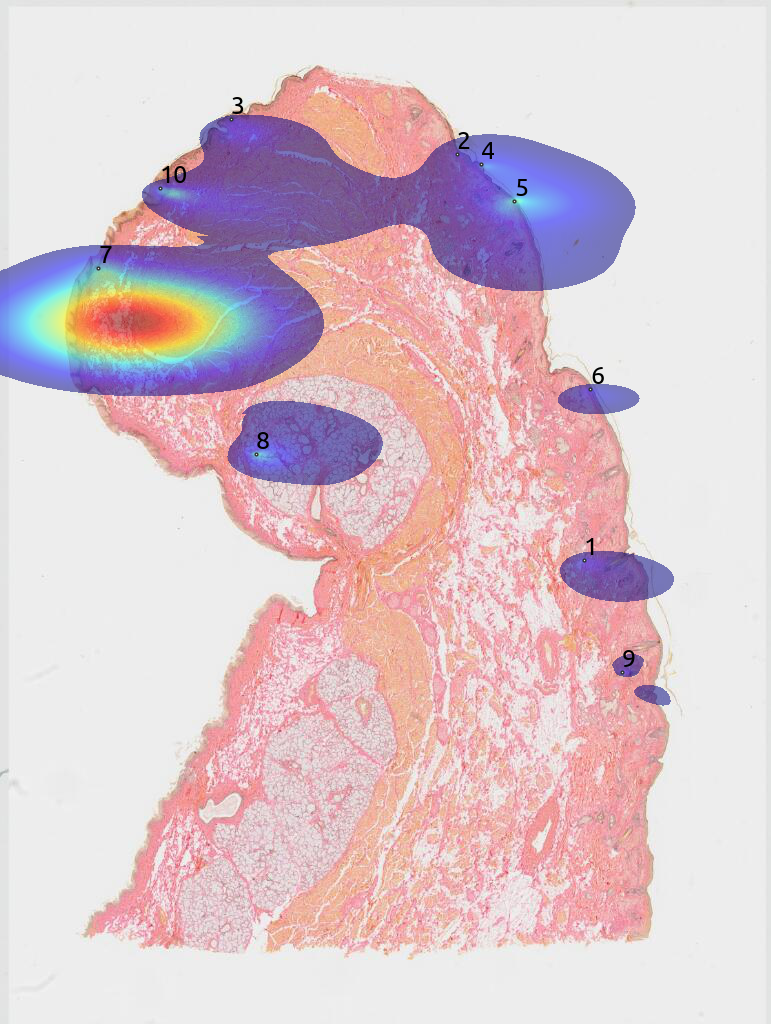
\includegraphics[width=\textwidth]{images/5501147_heatmap_basic.png}
            \caption{Raw}
            \end{subfigure}
            \begin{subfigure}[b]{0.19\textwidth}
            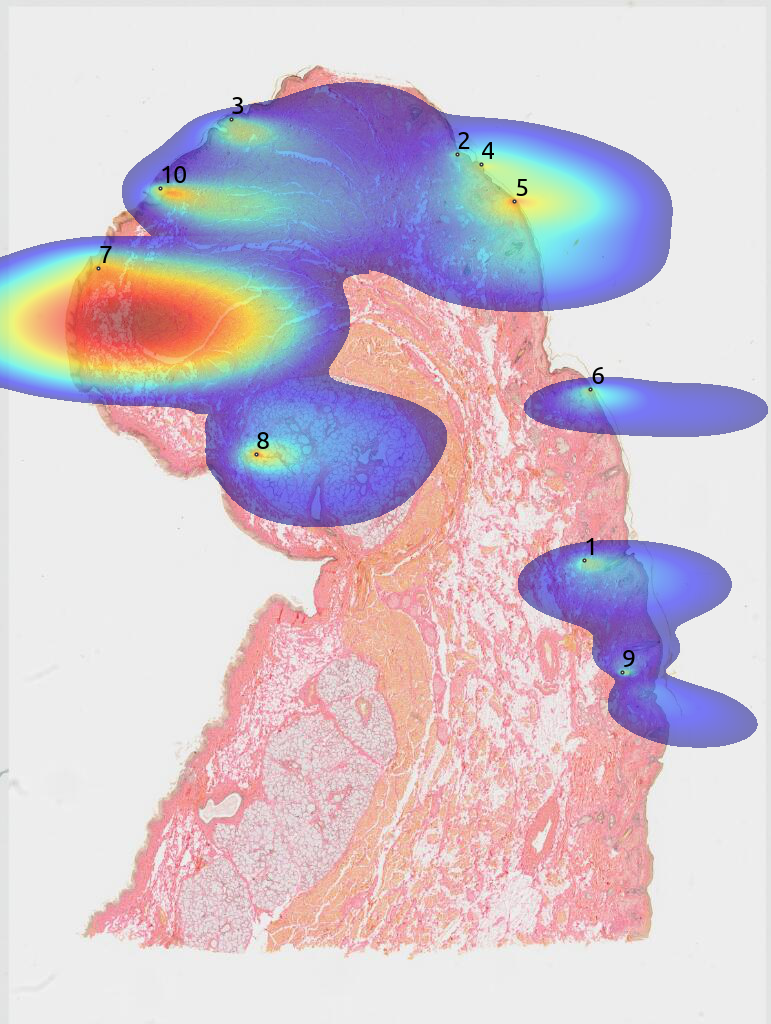
\includegraphics[width=\textwidth]{images/5501147_heatmap_ln.png}
            \caption{Logarithmic}
            \end{subfigure}
            \begin{subfigure}[b]{0.19\textwidth}
            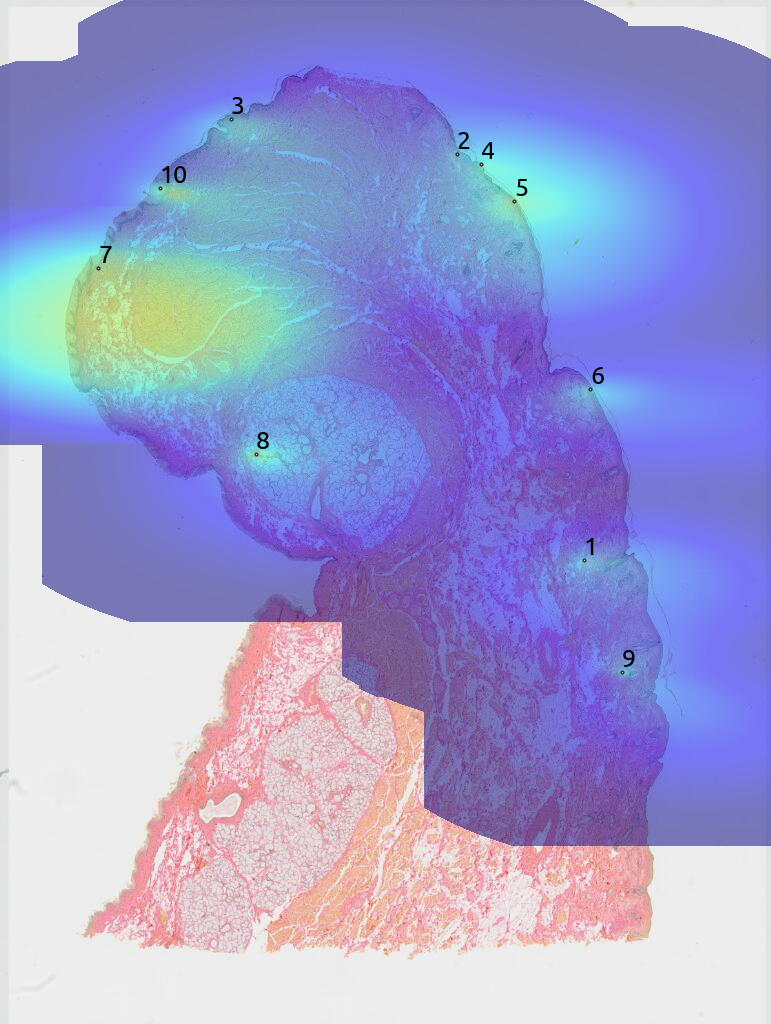
\includegraphics[width=\textwidth]{images/5501147_heatmap_image.png}
            \caption{Image Relative}
            \end{subfigure}
            \begin{subfigure}[b]{0.19\textwidth}
            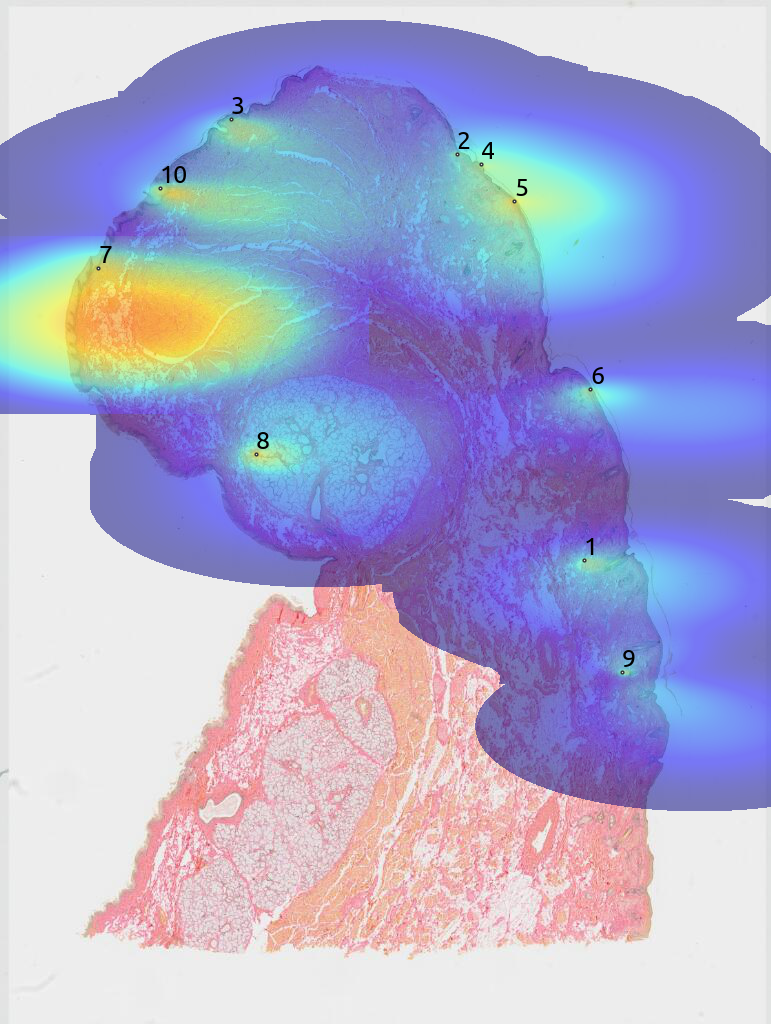
\includegraphics[width=\textwidth]{images/5501147_heatmap_user.png}
            \caption{User Relative}
            \end{subfigure}
            \begin{subfigure}[b]{0.19\textwidth}
            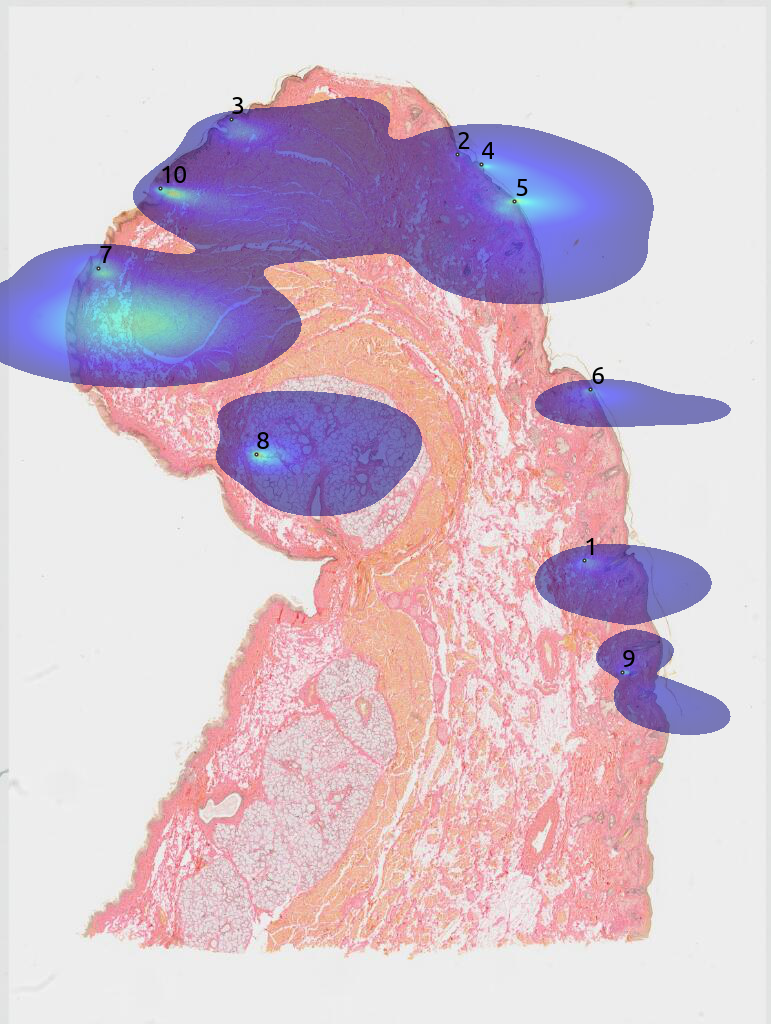
\includegraphics[width=\textwidth]{images/5501147_heatmap_reduced.png}
            \caption{Reduced}
            \end{subfigure}
            \caption{Example Figure of different Gazemaps}\label{fig:heatmaps}
        \end{figure}
        \item[\textbullet] \textbf{Output Scan Path Figures :} These figures represents the path taken by the students when they scan through an image.
        Another Idea that seems interesting is to observe a student's viewing order when looking at images.
        The idea is to draw arrow an plot that connects each position to the following position.
        After doing so for all the positions, it is possible to analyze the viewing order.
        Unfortunately, in most cases there are too many positions.
        This is why clustering is used to group up close positions in regards to time and space.
        K-Means clustering was implemented with K predetermined and ranging from 10 to 50 (K = 20 ideal).
        With this amount of clusters there may be a small loss in information but it allows the Scan Path to be observable.
        These clusters are arranged by the average time of their positions.
        Each cluster is also given a weight based on the number of positions that belong to it.
        This makes the scan path complete in a sense that it shows most of the needed information relating to the user's viewing order.
        The example in Figure \ref{fig:scanpath} shows the scan path associated to the same image and user pair as the Figure \ref{fig:heatmaps}.
        This shows that the zone where the student focused for a long duration was during the begining of the scan.
        The student may have been reading up on the course while keeping the image still.
        Following that, the student started visiting the different annotations.
        It's interesting to see that the student did not respect the order for the most part.
        The scan order is annotations 7, 8, 3, 2, 4, 1, 6, 5, 10,and finally 9.
          \begin{figure}[H]
          \centering
          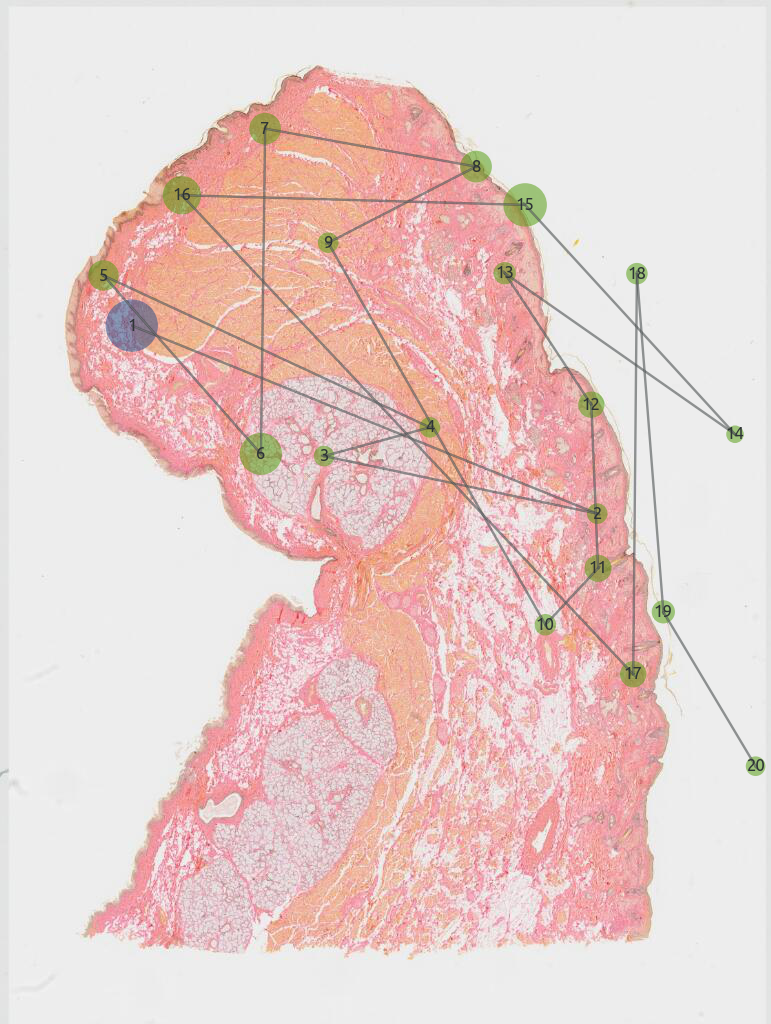
\includegraphics[width=.3\linewidth]{images/5501147_scanpath.png} 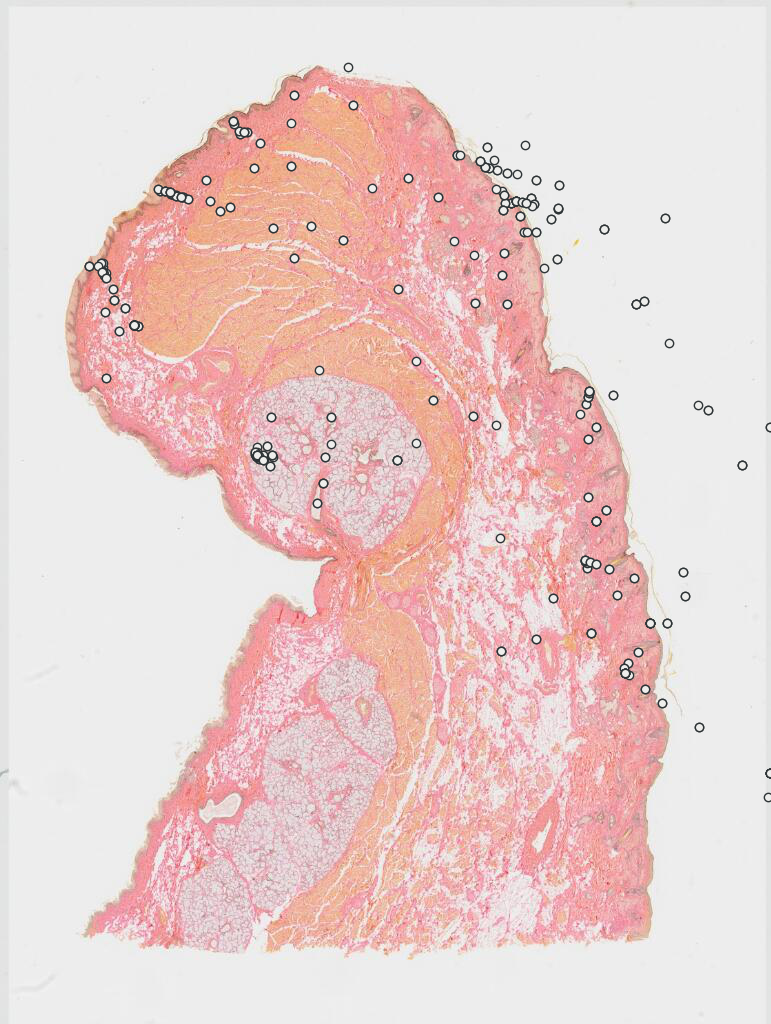
\includegraphics[width=.3\linewidth]{images/5501147_points.png}
          \caption{Scan Path and Raw Points Example}
          \label{fig:scanpath}
    \end{figure}
    \end{itemize}

    \begin{figure}[H]
      \centering
      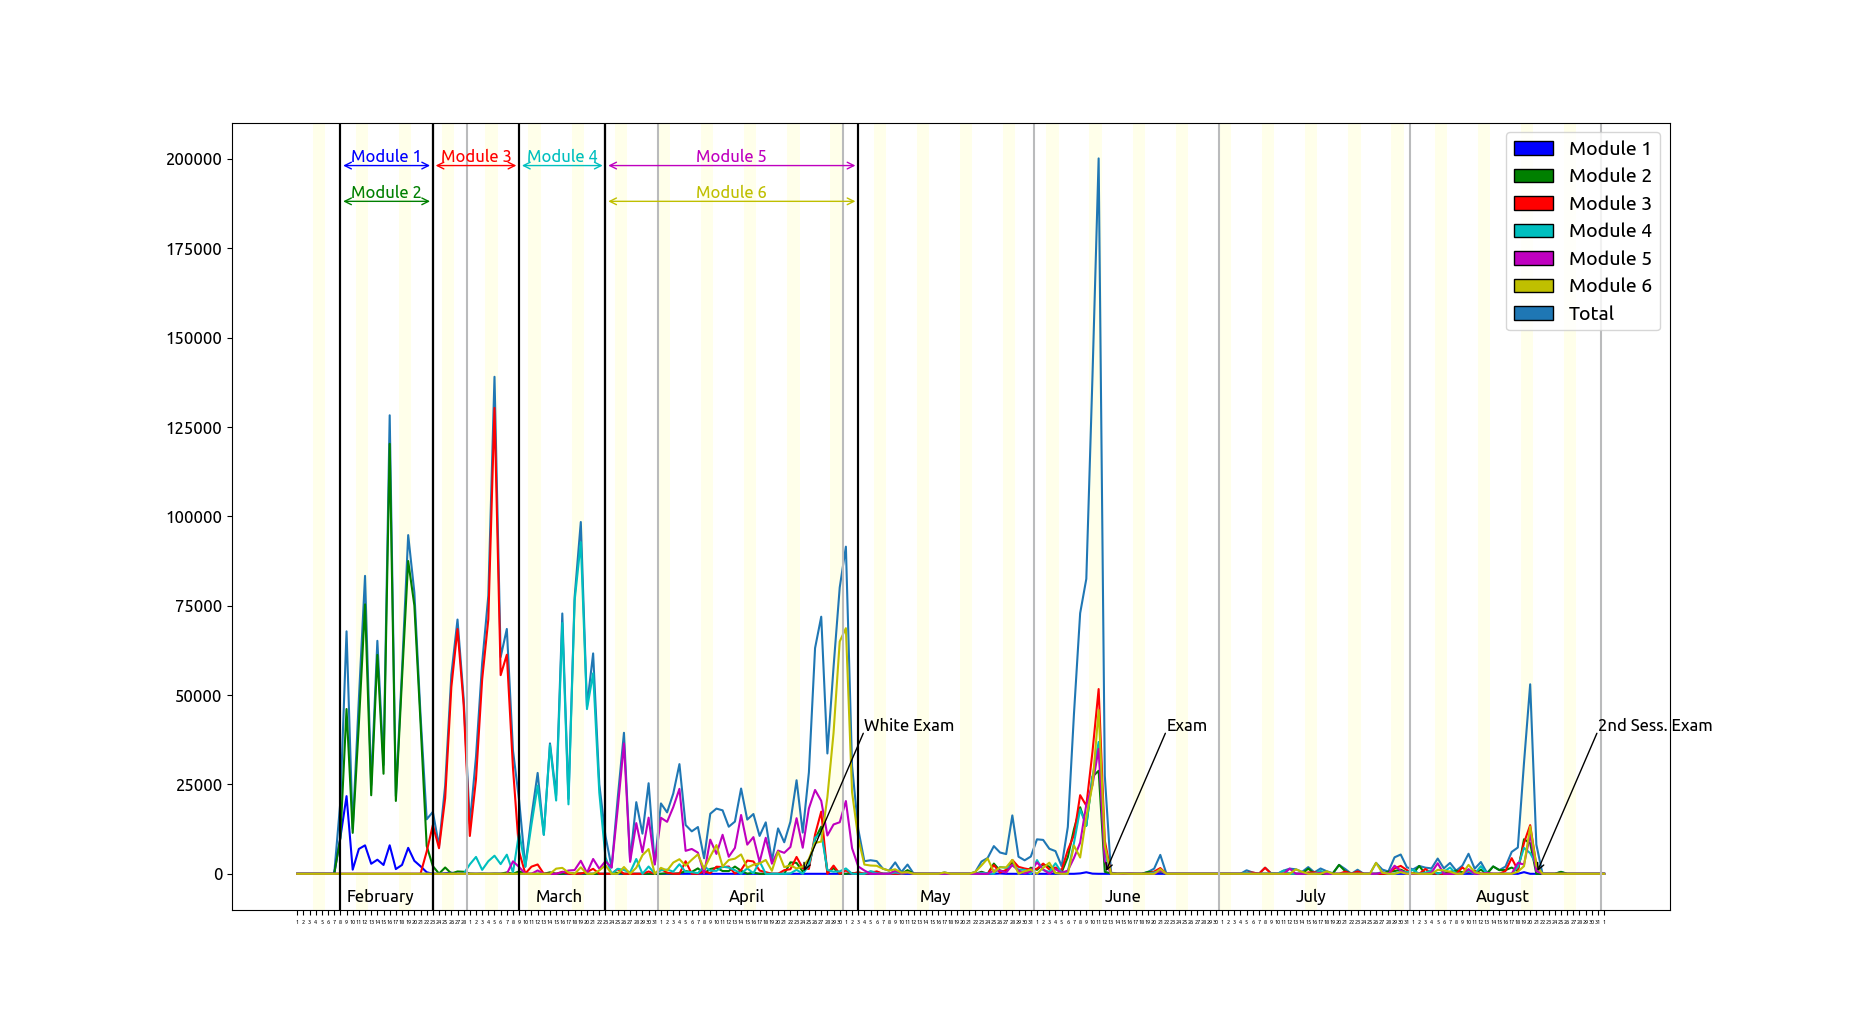
\includegraphics[width=.9\linewidth]{images/timelapse.png}
      \caption{Overall Student Activity over Time}
      \label{fig:timelapse}
    \end{figure}

    There are multiple options when running this component.
    When running the script it comes with one mandatory parameter \textbf{<project\_name>}.
    This is similar to the previous component where it corresponds to a certain project.
    Other optional prameters include :
    \begin{itemize}
        \item[\textbullet] \textbf{-I <images>} : The <images> field contains the address to a csv file containing a list of Cytomine image identifiers.
        Each row of the file contains one image identifier.
        This parameter is optional since it is possible to find image information from the disk.
        It is used if the user wants to use the component on a subset of images.
        \item[\textbullet] \textbf{-U <users>} : The <users> field contains the address to a csv file containing a list of Cytomine user identifiers.
        Each row of the file contains one user identifier.
        This follows the same principles than the images.
        \item[\textbullet] \textbf{-i <image>} : The <image> field contains a Cytomine image identifier.
        This is mutually exclusive with -I, where the component is ran on exactly one image.
        \item[\textbullet] \textbf{-u <user>} : The <user> field contains a Cytomine user identifier.
        This is mutually exclusive with -U, where the component is ran on exactly one user.
        The last two options are ideal when drawing heatmaps on a specific user/image pair.
        \item[\textbullet] \textbf{-M <output\_dir>} : This option allows the component to generate a CSV statistics file used for machine learning.
        The <output\_dir> field designates the folder where output learning data file will be saved.
        \item[\textbullet] \textbf{-m} : This option is mutually exclusive with the previous option.
        This also generates the statistics file but it is saved as \textit{../root/<project\_name>/learning\_data.csv}.
        \item[\textbullet] \textbf{-H} : This generates gazemaps (reduced) for all user/image pairs defined.
        They are saved in their respective directories.
        \item[\textbullet] \textbf{-S} : This generates scan paths for all user/image pairs defined.
        They are saved in their respective directories.
        \item[\textbullet] \textbf{-T} : This generates timelines for all users defined.
        They are saved in their respective directories.
        \item[\textbullet] \textbf{-R} :This generates raw point images for all user/image pairs defined.
        They are saved in their respective directories.
    \end{itemize}

    Overall, the component can be explained with the following diagrams (Figures \ref{fig:comp2} \& \ref{fig:comp2uml}).
    \begin{figure}[H]
      \centering
      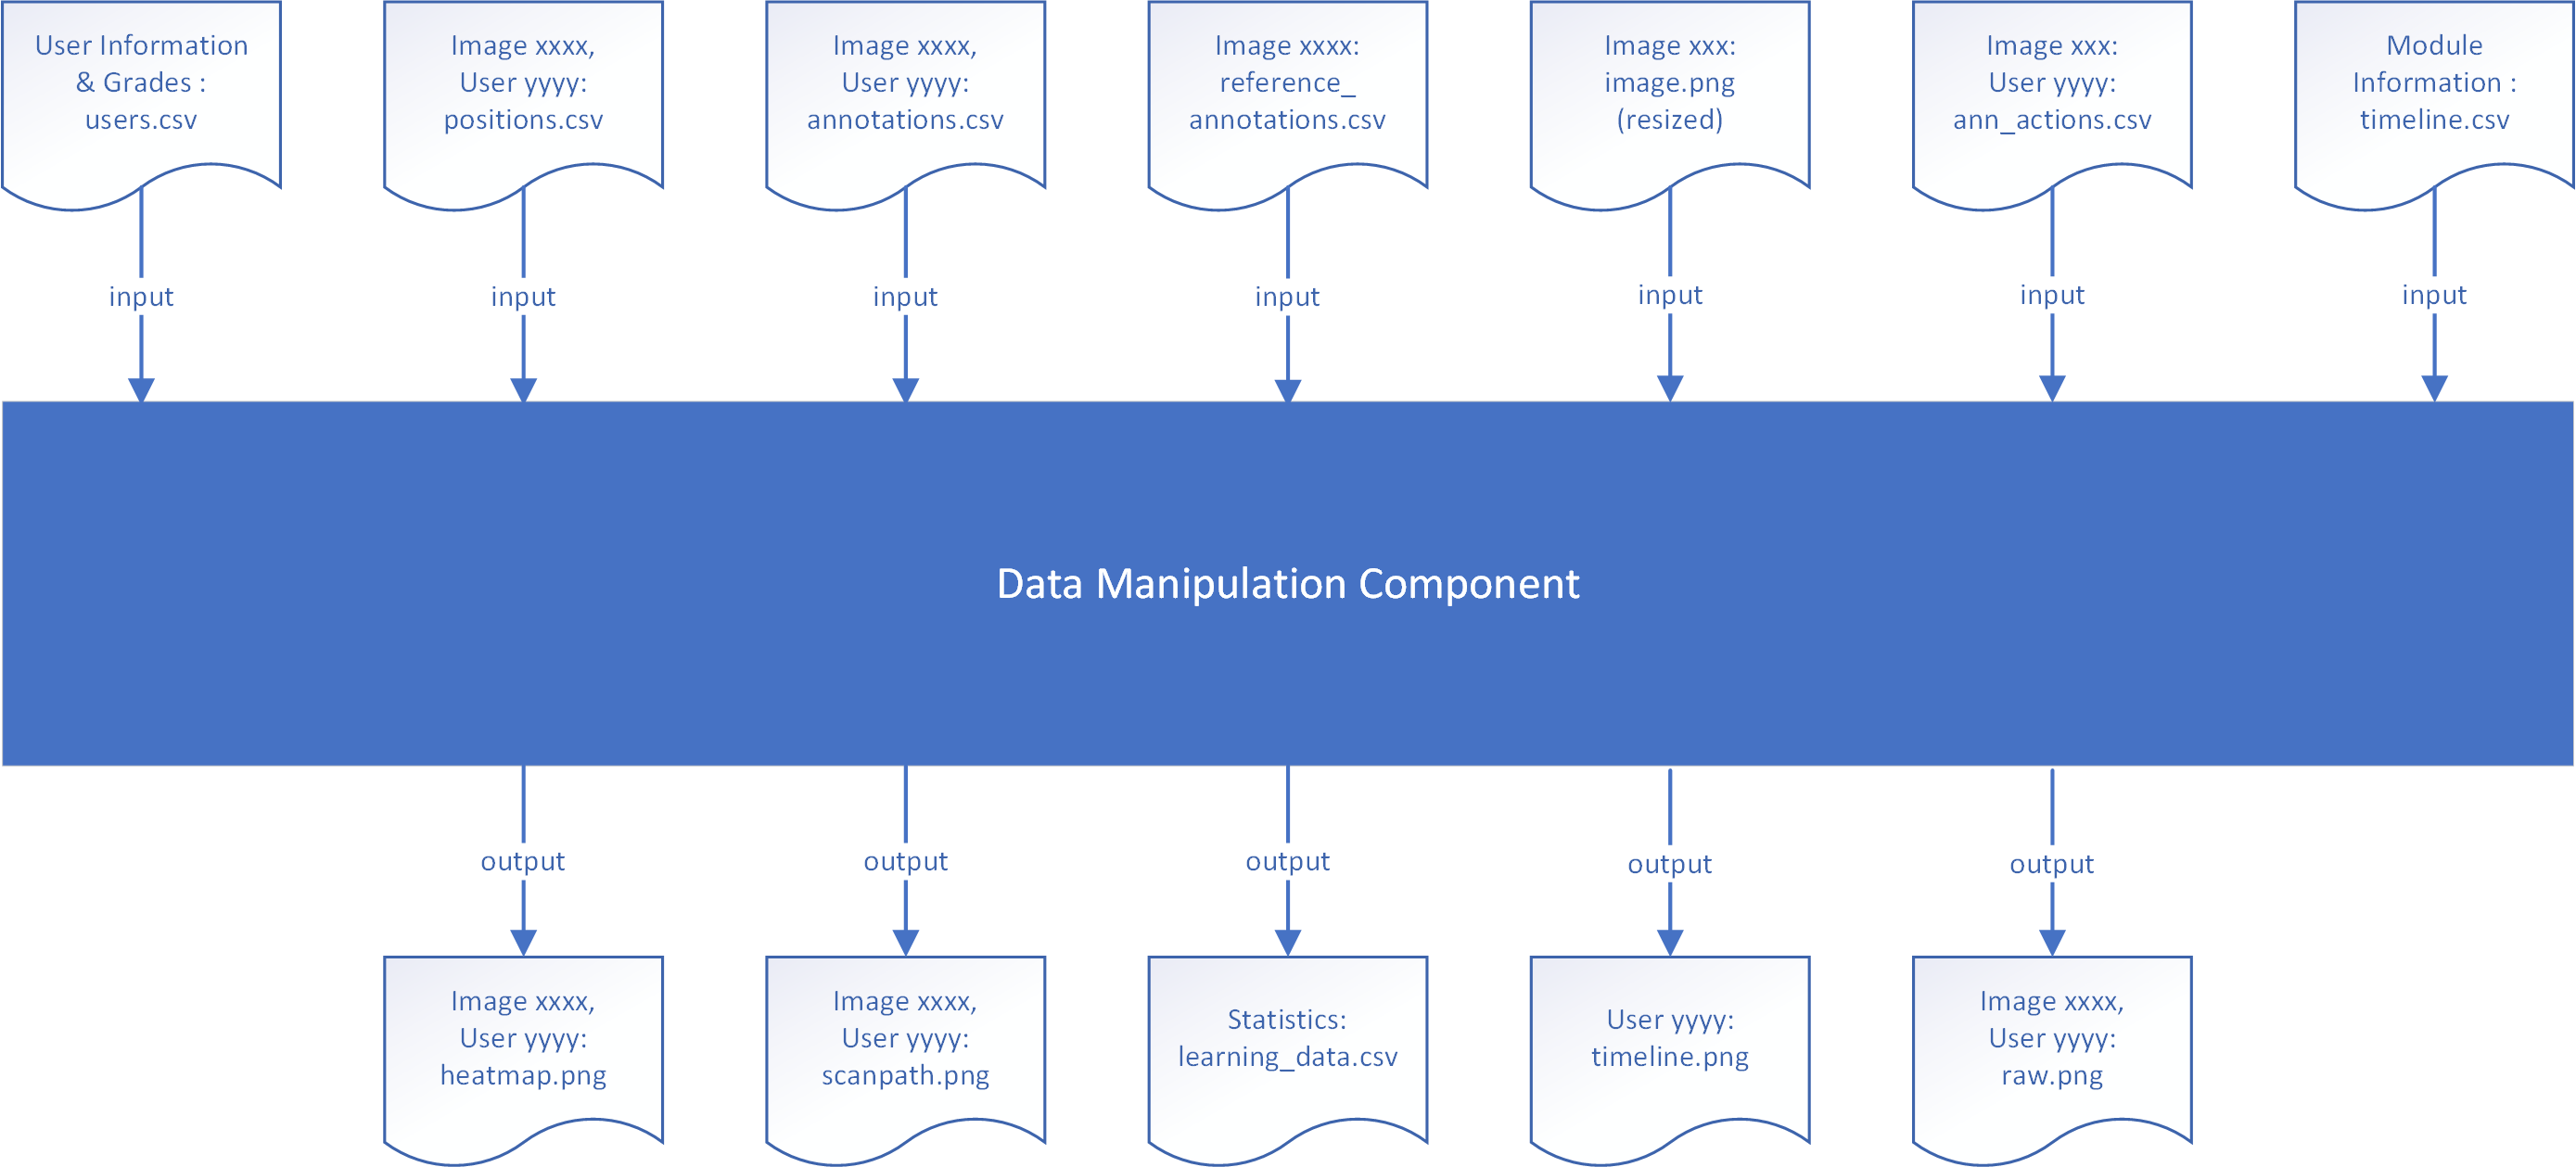
\includegraphics[width=.9\linewidth]{diagrams/module2.png}
      \caption{Data Manipulation Component}
      \label{fig:comp2}
    \end{figure}

    \begin{figure}[H]
      \centering
      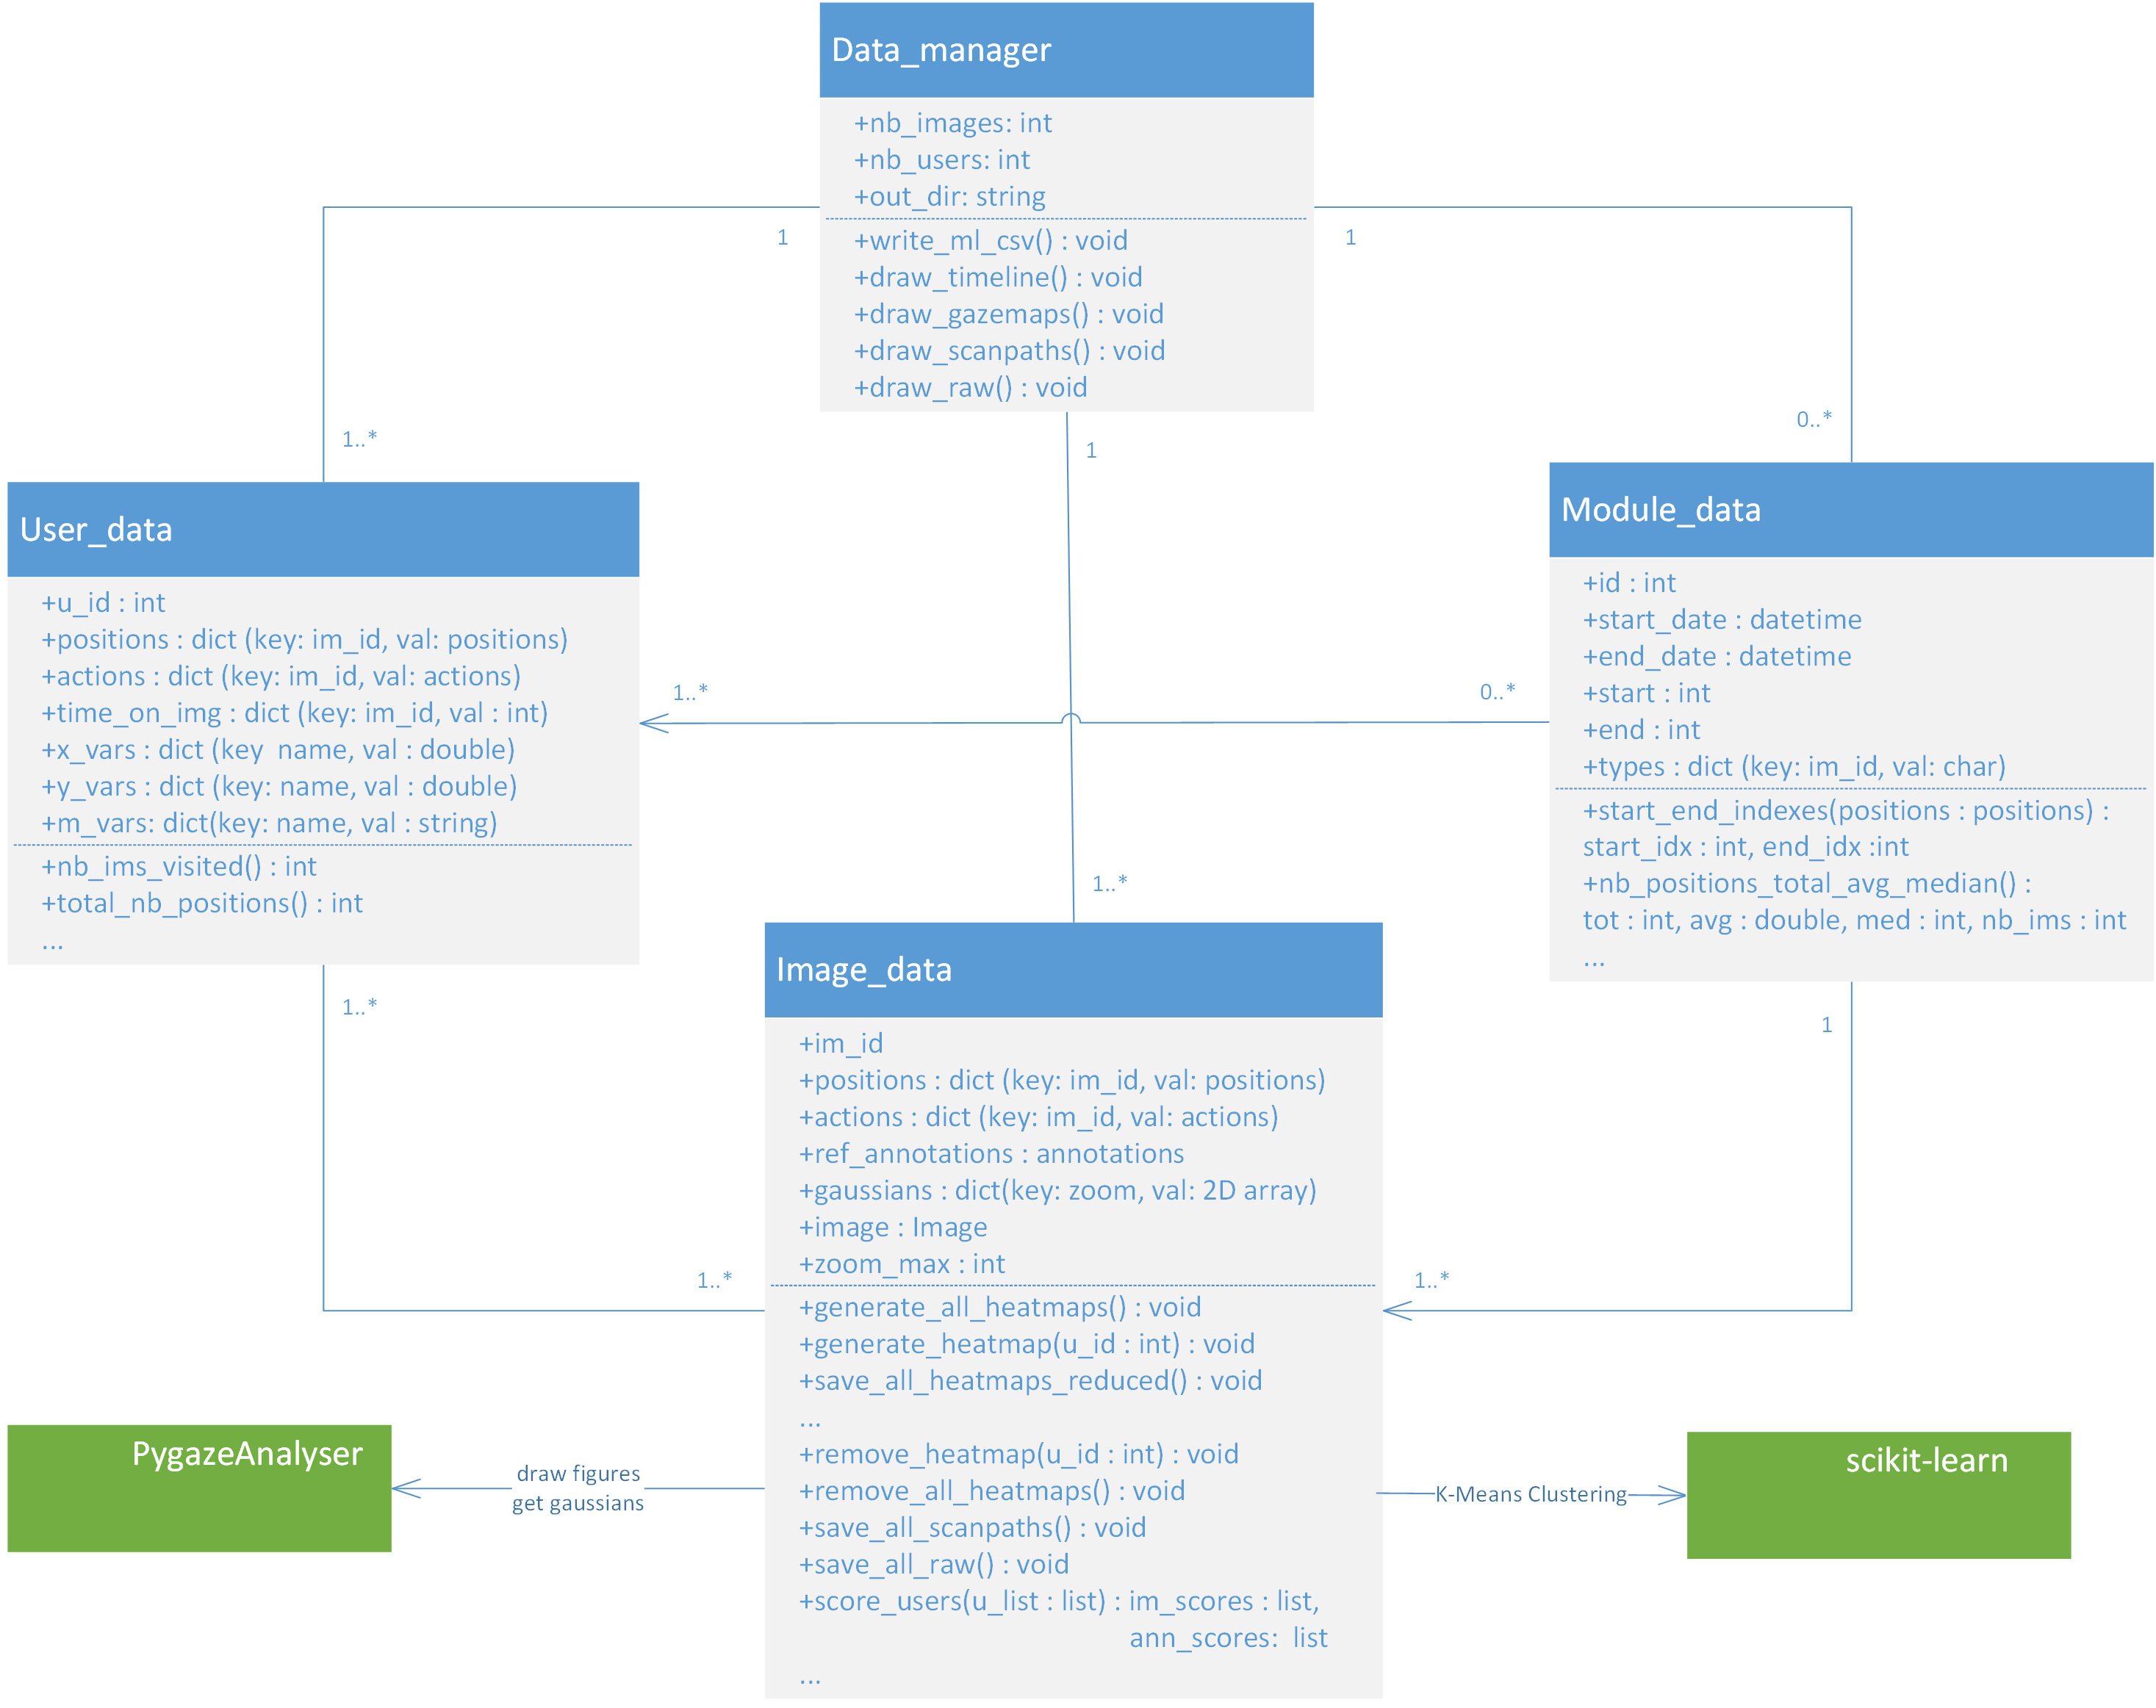
\includegraphics[width=.9\linewidth]{diagrams/module2uml.png}
      \caption{Data Manipulation Component UML}
      \label{fig:comp2uml}
    \end{figure}

    \subsection{Data Learning}

    This component has the objective of working with the output Feature file from the Data Manipulation component.
    As there many output variables, a Graphical Unit Interface (GUI) was implemented.
    This GUI shows the list of output variables that the user can chose from.
    The user then has the option to run two different methods :
    \begin{itemize}
        \item[\textbullet] \textbf{Building a full model :} All the feature variables have been fit into a ExtraTree Regressor with the selected output variable.
        From this model, statistics are extracted and visualized.
        This includes :
        \begin{itemize}
            \item \textbf{Feature Importance Histogram :} An ExtraTree Regressor outputs the impact of all the variables after the model is fit.
            Since there are over two thousand features, they can't all be visualized.
            Therefore, only the 80 most impactful features have visualized with an Histogram.
            Features are divided into 3 categories, those who were associated to specific Modules (in red), those who were associated to specific images (in green) and the more general features (in blue).
            This helps give a rough idea on the effect of certain features.
            \item \textbf{Image Importance Histogram :} This Histogram uses the features associated to specific images.
            For each image, the average feature importance is calculated.
            This is then shown in the Histogram.
            Images were also split into categories based on the module they belong to.
            The each category is represented by a color.
            This helps determining what images and modules had the biggest impact on the grades obtained.
            \item \textbf{Variable Correlation Scatter Plot :} This scatter plot compares the output variable to a top feature.
            This visualizes the relation between those two variables.
            This includes aline with a Pearson Correlation to represent the slope of the of the relation.
        \end{itemize}
        \item \textbf{Running a Leave-One-Out Cross Validation :} With a total of N individuals, the model is fit N times with N-1 individuals.
        For each iteration, the individual left out will be tested with the model.
        With this, the learned value is returned and is compared with the original value.
        After each iteration, statistics were derived from the results :
        \begin{itemize}
            \item \textbf{Mean Absolute Error (score):} The average absolute error obtained by the cross-validation.
            \item \textbf{Score of the Median Model :} The cross-validation is compared to a method that does a leave-one-out cross validation of the set by just taking the median value.
            This is to give confirmation on whether or not the results of the ExtraTree Regressor are determined somewhat randomly.
            \item \textbf{Score Difference :} This is the difference between the two previously mentioned scores.
            The higher the difference, the better.
            \item \textbf{P-Value :} The P-value of the cross validation results with the original output variables.
            This method uses the T-Test to see if the two variables are significantly different from each other.
            The P-value is valued from 0 to 1 with 1 meaning that the sets are exactly the same and 0 meaning the sets are completely different.
            In this case, the ideal P-value would be 0.95.
            \item \textbf{P-Value of the Median Model :} Similar to the previous P-Value but applied to the median model.
        \end{itemize}
        This leads to the implementation of statistics that are visualized in graphs:
        \begin{itemize}
            \item \textbf{Scatter Plot :} This compares the learned results with the output variables.
            It includes four Lines.
            The first line (in red) represents $x = y$, the best possible outcome for the learning.
            The goal is to have the most accurate regression.
            This happens when the scattered points are closest to that line.
            The next two (in green) represents $x = y \pm score$, this is to give a interval where the error for the scattered points inside are less than the mean.
            The last (in blue) represents the slope of the relation between the two variables.
            It includes a Pearson Correlation to better understand the slope of the line.
            \item \textbf{Box Plot :} This visualizes the error between the learned results with the output variables.
            In this case, it draws the median error, the two quartiles Q1 (separating the 25 \% with the lowest error with the rest) and Q3 (seperating the 75 \% with the lowest error with the rest), and the two whiskers.
            The whiskers have a reach that are 1.5 times the inter-quartile range.
            This means that any error outside the reach of the whiskers would be deemed extreme cases.
            These cases are related to really high error values.
        \end{itemize}
    \end{itemize}

    The ExtraTree (Extremely Randomized Tree) regressor is a class that fits a number of randomized decision trees on many sub samples of the population (see ~\cite{extratree}).
    This method uses averaging to to improve learning accuracy all while controlling over-fitting.
    It is therefore considered a Ensemble Method.
    The Regressor has been implemented with scikit-learn ~\cite{scikit-learn}.
    It has been configured with the following parameters :
    \begin{itemize}
        \item[\textbullet] \textbf{Number of Estimators : 10 000}\\
        Represents the number randomized trees generated.
        \item[\textbullet] \textbf{Max depth : None}\\
        The max depth of the trees.
        \item[\textbullet] \textbf{Bootstrap : False}\\
        Whether or not bootstrapping was implemented.
        Bootstrapping implements sampling with replacement within the training set.
        \item[\textbullet] \textbf{Max Features : Auto ( = Number of Features)}\\
        Max number of features that can be used by the randomized tree.
        \item[\textbullet] \textbf{Max leaf Nodes : None}\\
        The maximum number of leaf nodes that be present in a tree.
        \item[\textbullet] \textbf{Minimum Impurity Decrease : 0.0}\\
        A node will be split if the impurity is less than the minimum impurity decrease value.
        Threshold for early stopping tree growth.
        \item[\textbullet] \textbf{Minimum Samples Leaf : 10}\\
        The minimum number of samples required at a leaf node.
        \item[\textbullet] \textbf{Minimum Samples split : 2}\\
        The minimum number of samples required to split an internal node.
        \item[\textbullet] \textbf{Minimum Weight Fraction Leaf : 0.0}\\
        Minimum weighted fraction of the sum total of all weights (of all input samples) required at a leaf node.
        If 0.0, samples have equal weights.
        \item[\textbullet] \textbf{Criterion : msq - Mean Square Error (mae is too slow)}\\
        The method to measure the quality of a split.
        \item[\textbullet] \textbf{Out-of-bag Score : False}\\
        Whether out-of-bag samples are used to estimate how well unseen data is fitted to a regression line.
    \end{itemize}
    Since the ExtraTree regressor handles overfilling by itself, it is useful to have many estimators when handling a vast amount of features.
    Also, with many estimators the method will converge to output the best possible results where ExtraTrees are are concerned.
    It is one of the more ideal choices for such a data set for many reasons :
    \begin{itemize}
        \item[\textbullet] The high number of features paired with a small number of individuals.
        Ensemble methods are ideal in this scenario.
        \item[\textbullet] Easy to interpret (variable importance for example).
        \item[\textbullet] The data comes all at once, so the tree only needs to be fit once.
        \item[\textbullet] Good for modeling linear interactions.
        Most relations studied in this project are linear.
        With the sample size, it is risky to try and infer more complex relations.
    \end{itemize}

    \section{Performance}

    Like mentioned before, the tool as a whole can take a while to executed depending on the parameters set.
    The device used for running and testing this tool has the following properties:
    \begin{itemize}
        \item[\textbullet] \textbf{Processor} : Intel Core i7-6700M/PCIe/SSE2
        \item[\textbullet] \textbf{RAM} : 16 GB
        \item[\textbullet] \textbf{Disk} : 1 TB (For storing data, about 48 GB used for this tool)
    \end{itemize}

    The data acquisition component is hard to measure.
    Since the Cytomine server ran locally and that there are no other users using the application, the download time measured may be quicker than it should be.
    For the project GOLD with 78 images and 395 users, it takes about 6 hours to acquire all the data.
    Conversely, for the SILVER project with 75 images and 85 users, it only takes about 16 minutes.
    Overall most operations on the SILVER project are much quicker.
    Overall, users are more active in the GOLD project.
    They have more positions, it influences directly the complexity of most operations.\\


    For the data manipulation component, most operations done on a image/user pair scale linearly with the number of positions.
    Outputs measured include :
    \begin{itemize}
        \item[\textbullet] \textbf{Generating a reduced Gazemap}  : With $N$ positions and an image with a height and width of $h$ and $w$ respectively, heat values need to be calculated for each pixel.
        How a heat value is calculated for a pixel is shown in section \ref{enum:score} when calculating a score of an annotation.
        For a pixel the complexity is $O(N*log(N))$.
        The most costly operation is sorting the list.
        This is donne for each pixel, therefore the final complexity is $O(h*w*N*log(N))$.
        With an image that has a resolution of about 1024x1024, it heavily relies on the number of positions.
        Overall it can take from 5 seconds up to about 2 minutes for users that do not have an absurd amount of positions.
        \item[\textbullet] \textbf{Generating a scan Path} : $N$ positions need to be clustered into about 20 areas.
        Using K-means clustering with scikit-learn, the average complexity is $O(K*N**T)$ where $T$ is the number of iterations.
        In this case, $T$ is set at 300.
        When drawing the scan path itself, it's much quicker because positions are reduced to 20 zones.
        Overall operations are done almost instantly, the biggest burden is saving the image to the disk.
        \item[\textbullet] \textbf{Generating a raw Point image} : Drawing $N$ raw points with no prior manipulation has a complexity of $O(N)$.
        Overall operations are also done instantly.
        \item[\textbullet] \textbf{Generating Timelines} : The total number of positions (from all the images) for each day needs to be calculated for each user, therefore it has a complexity of $O(N)$.
        This is slightly slower than the previous two methods because as a whole, users can have many positions.
        \item[\textbullet] \textbf{Generating Statistics File} : Generating this file requires the calculation of many features.
        Most features are calculated instantly, however the score variables shown in section \ref{enum:score} can take significantly more time.
        For an image/user pair, if there are no reference annotations, scores are calculated as the average score of each pixel.
        Unfortunately, it's the same complexity as generating a Gazemap in this case.
        However, there are not many images with no reference annotation.
        Overall for the GOLD project, it can take 4 hours to generate this file as a whole.
        However, without those score features it takes less than 20 minutes.
    \end{itemize}

    As for the data learning component, building a full model takes about 30 minutes while the cross-validation takes about 8 to 14 hours to run.
    This depends on the variable that is learned. \\

    Overall, most operations cannot be done in real time.
    If this were to be added to the Cytomine Application, a user requesting a Gazemap may need to wait.

\chapter{Data Analysis}

	\section{Experiments} \label{experiments}


    Even though the data was obtained for both the GOLD and SILVER projects, the experiments were on run on the GOLD project.
    This is due to the many constraints given by the SILVER project including the sample size and the lack of results (student grades).
    The goal for most experiments is to learn a specific grade the student obtained based on all the information gathered in the Data Manipulation component.
    There were over 2000 features generated, where each one can weigh in on the prediction.
    These features were used to learn over 13 grades including the final grade obtained by these students (first session).\newline


    Due to the nature of the dataset, regression trees were the most ideal.
    The somewhat small dataset paired with a large amount of features is a big constraint to work with.
    Therefore, Ensemble methods were used and tested.
    This includes Random Forest regression and Extra Trees regression using sklearn.\newline

    The Learning component is given a statistics file containing rows of students paired with their features.
    The features are split into three categories :
    \begin{itemize}
\item[\textbullet] \textbf{M} : Meta-data variables, these variables have no statistical significance.
These variables usually contain basic information on the users.\\
\item[\textbullet] \textbf{X} : Variables with statistical significance, these variables mostly include data extracted from the Cytomine website.
Either individual image variables or variables on the set of images.
These variables are used in the machine learning model as input variables.\\
\item[\textbullet] \textbf{Y} : Result variables, these variables is what the algorithm is attempting to guess using the  \textbf{X} variables.
These variables are used in the machine learning model as output variables. In this case, they are the students' grades.\\
\end{itemize}

    With this, a couple experiments have been ran.
    For each Y variable (that will be described in the next sections), the model was built fully for the first analysis.
    The second analysis, a leave-one-out cross validation was ran.
    The goal is to give insight on different user behaviors.
    Hopefully, these experiments will prove to be useful.

    \section{Data Set} \label{Data_Set}

    	\subsection{Students}
    Like mentioned earlier, there are a total of 395 students in the data set.
    Students are defined by their features and the grades obtained.
    These student followed the course HISL054, "General histology and alternative experimentation methods that do not use animals" at the University of Liege during the academic year 2016-2017.
    Most of the work done by the students is done online using the MOOC and Ecampus.
    Ecampus is a website used by students and teachers of the University of Liege to exchange information used for courses.
    In fact all of the assignments for this course are explained on Ecampus.
    The issue with this is that it is a different entity from the MOOC and therefore is not ideal for fetching information.
    But it is not much of a problem because there is nothing to retrieve about students on Ecampus that is not already known.\newline

    When applying machine learning techniques, students with a 0/20 were taken out of the sample because they default to signing the exam.
    Since there are too few that do so, there is not enough information to find correlations between people who sign and the features.
    Keeping students who sign also increases the error rate because they are outliers.
    The goal is to guess how well the exam would have went for the students.
    If the student decides not to bother with taking the exam, it is a lost sample.\newline

    	\subsection{Teacher Input : Grades}

    %% QROL - Question a Reponse Ouverte Longue
    %% QCM - Question a choix multiples
    %% QCL - incidence de coupe et identification

	The students are evaluated by multiple exams and quizzes, these take the form of:
    \begin{itemize}
    \item[\textbullet]  \textbf{QCM : Multiple choice question test.}
    Students are given questions and have to respond with 1 out of the 9 (or less) options.
    They have to set a degree of certainty for each response.
    The exam results are then calculated by a machine.
    The students are also given more boxes to answer in case they make a mistake the first time.(Figure \ref{fig:qcm})
    \begin{figure}[H]
    \centering
     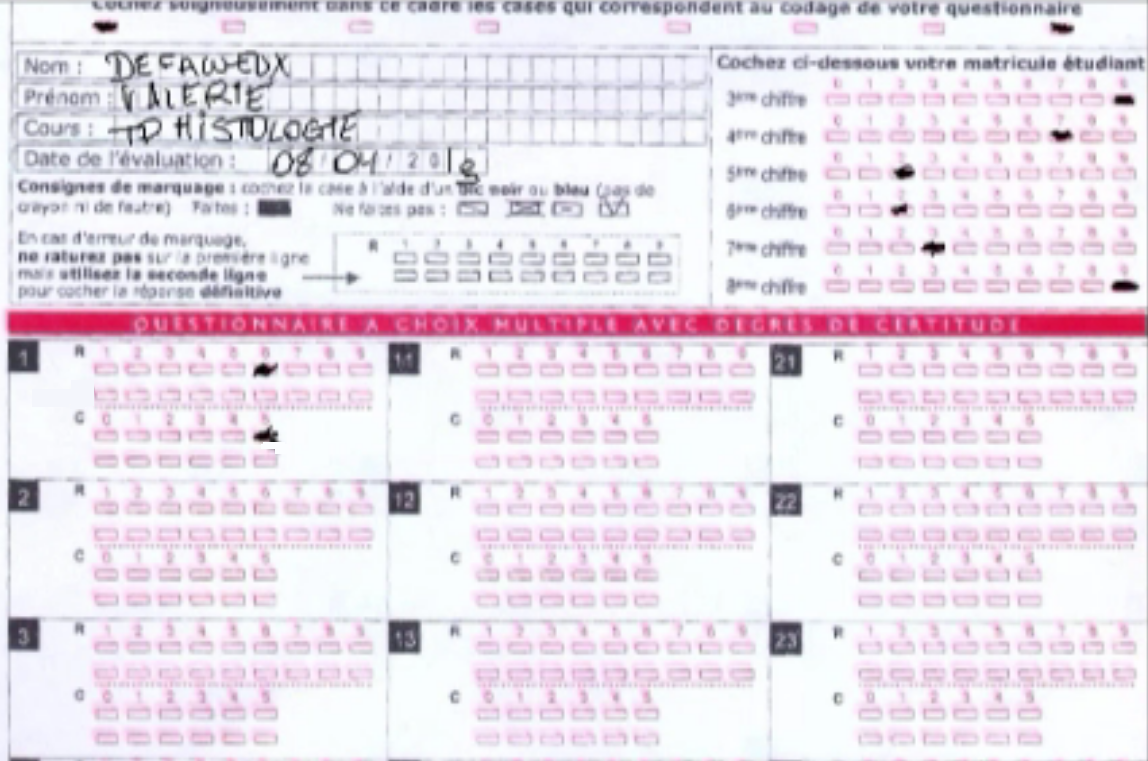
\includegraphics[width=0.4\linewidth]{images/exam_qcm.png}
     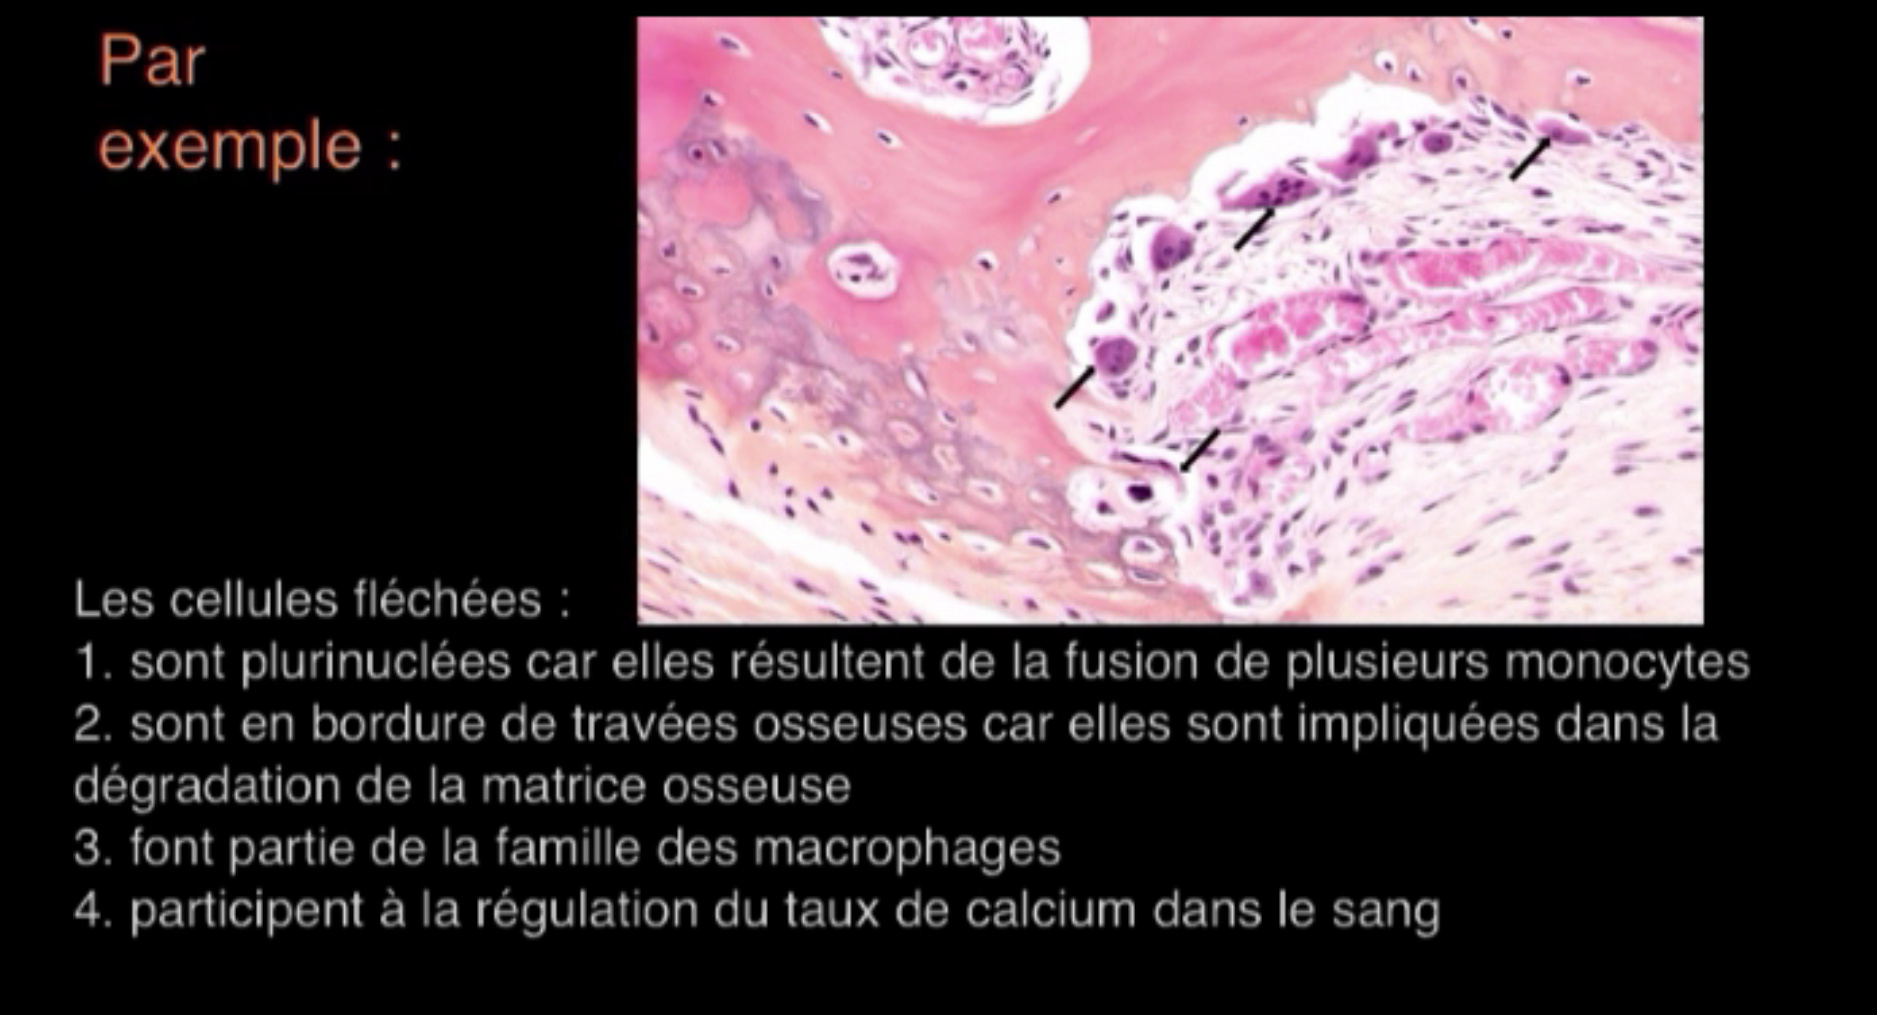
\includegraphics[width=0.5\linewidth]{images/exam_qcm2.png}
     \caption{QCM sheet and question example}
     \label{fig:qcm}
    \end{figure}
	\item[\textbullet]  \textbf{QCL : Identification and Incidence test.}
	Graded similarly to a QCM, the students are given multiple questions to answer and they have to fill out a form.
	The are a couple differences.
	Each question is split into two, the identification and the incidence.
	For the identification, the students have to identify an object on an image.
	They are given an exhaustive list of possible answers ranging from cells to tissues.
	Each answer contains is associated to a 3 digit code that they need to write on the form.
	For the incidence, the students needs to identify how the observed object "was cut".
	There are a total of 3 possible answers, transversal, longitudinal, and undetermined.
	The answer is written on the form under the identification answer.(Figure \ref{fig:qcl})
      \begin{figure}[H]
    \centering
     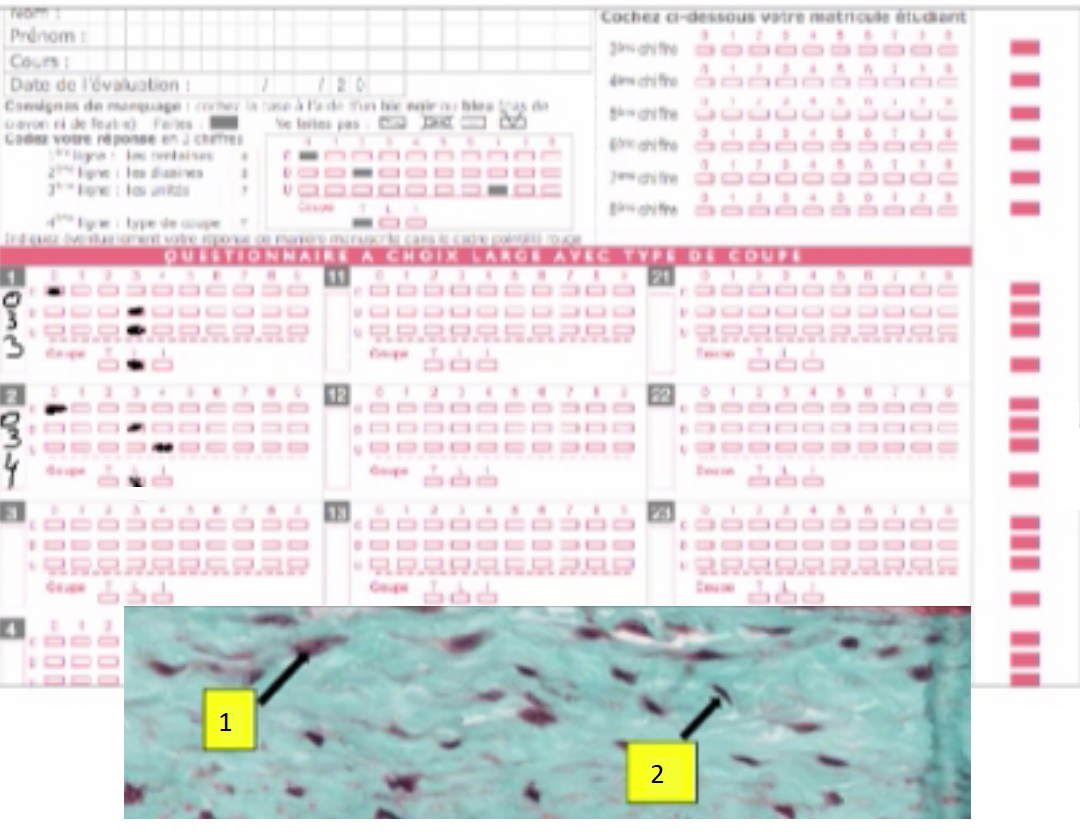
\includegraphics[width=0.42\linewidth]{images/exam_qcl2.png}
     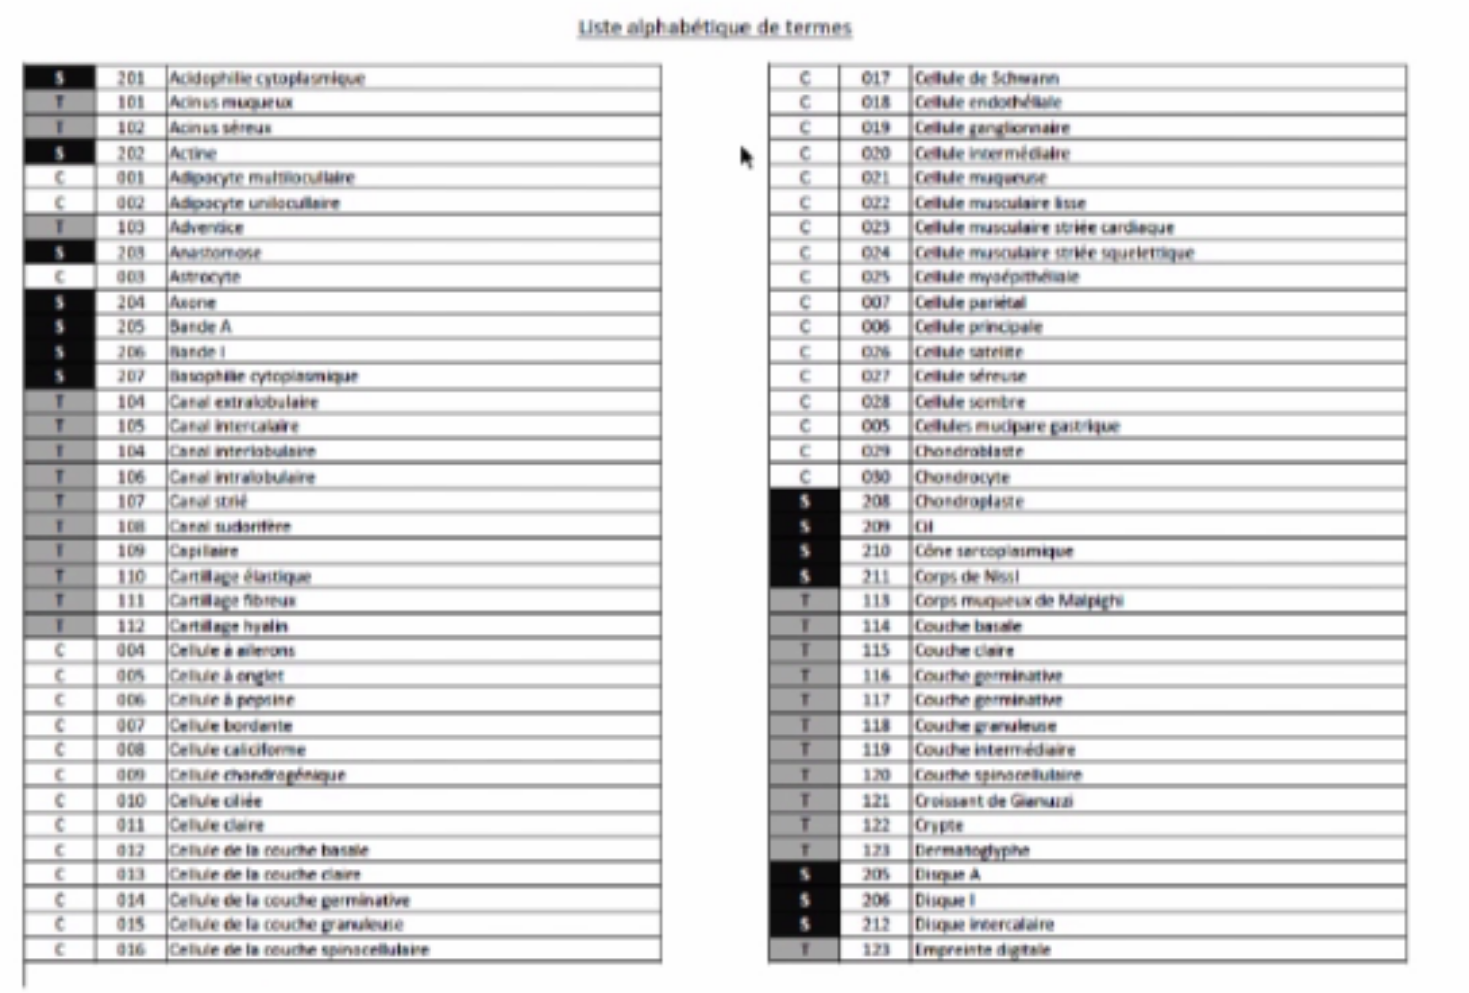
\includegraphics[width=0.5\linewidth]{images/exam_qcl.png}
     \caption{QCL sheet with question example and list of answers}
     \label{fig:qcl}
    \end{figure}
	\item[\textbullet]  \textbf{QROL : Long answer open question test.}
	Students are to write and explain their answers in a detailed fashion. (Figure \ref{fig:qrol})
          \begin{figure}[H]
    \centering
     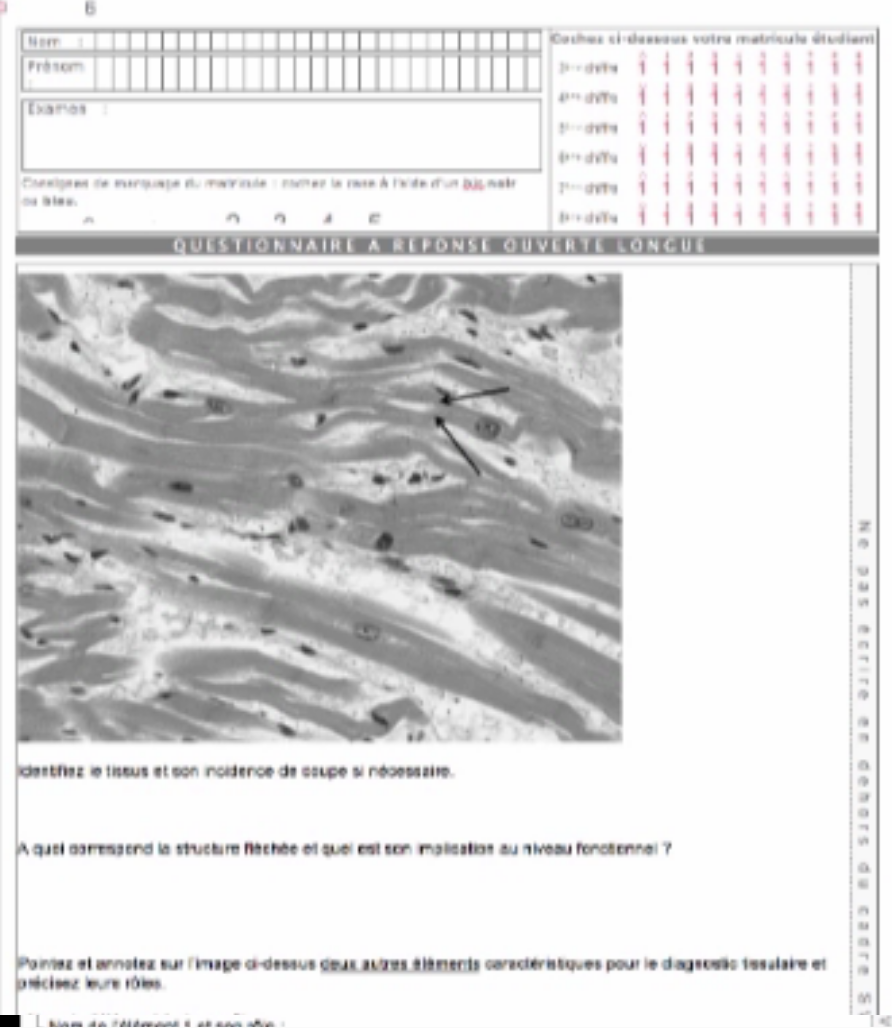
\includegraphics[width=0.45\linewidth]{images/exam_qrol.png}
     \caption{QROL sheet with a set of questions}
     \label{fig:qrol}
    \end{figure}
    \end{itemize}

    These variables will be denoted as \textbf{Y} variables for output.
    Out of the 13 results associated to the students, 3 were white tests given as a practice tool :
    \begin{itemize}
    \item[\textbullet]  QCL identification white test.
	\item[\textbullet]  QCL incidence white test.
	\item[\textbullet]  Practical QCM white test.
    \end{itemize}
    Similarly, 7 graded exams and quizzes were given to students with 3 being theoretical and 4 being practical.
    Something to note for the practical exam is that there are 2 different exam forms for the QCM and the QRL. This means that half the students are given different questions from the other half.
    The list of exams include:
    \begin{itemize}
    \item[\textbullet]  QROL1 theory (10\%).
    \item[\textbullet]  QROL2 theory (10\%).
    \item[\textbullet]  QCM theory (30\%).
    \item[\textbullet]  QCM practical (20\%).
    \item[\textbullet]  QROL practical (10\%).
    \item[\textbullet]  QCL identification Practical (16\%).
    \item[\textbullet]  QCL incidence Practical (4\%).
    \end{itemize}
    Finally, based on the previous results given, there are:
    \begin{itemize}
    \item[\textbullet] Total Theory (50\%)
    \item[\textbullet] Total Practical (50\%)
    \item[\textbullet] global Grade (100\%)
    \end{itemize}

    Most of the experiments are done using one of these grades as Y variables.
    In later experiments, some variables will be set as features.
    The learning of final grades using white test results as bonus features (\textbf{X} variable) could yield better results.
    Learning theoretical grades while also using practical grades and vice versa can also give some interesting results. \\

    Statistics can be derived for each variable :\\

    \begin{center}
      \begin{tabular}{| p{1cm} | p{0.6cm} | p{0.6cm} | p{0.6cm} | p{0.6cm} | p{0.6cm} | p{0.6cm} | p{0.6cm} | p{0.6cm} | p{0.6cm} | p{0.6cm} | p{0.6cm} | p{0.6cm} | p{0.6cm} | }
      \hline
      & \tiny{White Test QCL ID} & \tiny{White Test QCL IC} & \tiny{White Test QCM} & \tiny{QROL Theory 1} & \tiny{QROL Theory 2} & \tiny{QCM Theory} & \tiny{QCM Practical} & \tiny{QROL Practical} & \tiny{QCL ID Practical} & \tiny{QCM IC Practical} & \tiny{Total Theory} & \tiny{Total Practical} & \tiny{Global Grade}\\ \hline
      \tiny{Minimum} & \tiny{1.33} & \tiny{1.33} & \tiny{0.36} & \tiny{0.44} & \tiny{0.67} & \tiny{3.43} & \tiny{3.16} & \tiny{0.29} & \tiny{1} & \tiny{2} & \tiny{2.59} & \tiny{2.01} & \tiny{1.68}\\ \hline
      \tiny{Maximum} & \tiny{18.67} & \tiny{20} & \tiny{19.64} & \tiny{20} & \tiny{20} & \tiny{17} & \tiny{17.32} & \tiny{18.82} & \tiny{20} & \tiny{20} & \tiny{17.8} & \tiny{17.99} & \tiny{17.85}\\ \hline
      \tiny{Average} & \tiny{8.09} & \tiny{12.17} & \tiny{10.18} & \tiny{10.67} & \tiny{12.16} & \tiny{10.05} & \tiny{10.88} & \tiny{8.6} & \tiny{11.15} & \tiny{15.03} & \tiny{10.56} & \tiny{10.81} & \tiny{10.63}\\ \hline
      \tiny{Median} & \tiny{8} & \tiny{13.33} & \tiny{10.31} & \tiny{10.75} & \tiny{12.83} & \tiny{10.03} & \tiny{10.8} & \tiny{7.93} & \tiny{11} & \tiny{15} & \tiny{10.75} & \tiny{10.76} & \tiny{10.67}\\ \hline
      \tiny{Variance} & \tiny{14.09} & \tiny{17.67} & \tiny{13.3} & \tiny{16.78} & \tiny{19.51} & \tiny{6.41} & \tiny{7.93} & \tiny{18.92} & \tiny{16.48} & \tiny{9.35} & \tiny{8.46} & \tiny{9.92} & \tiny{8.64}\\ \hline
      \tiny{Standard Deviation} & \tiny{3.75} & \tiny{4.2} & \tiny{3.36} & \tiny{4.09} & \tiny{4.41} & \tiny{2.53} & \tiny{2.81} & \tiny{4.34} & \tiny{4.06} & \tiny{3.05} & \tiny{2.9} & \tiny{3.15} & \tiny{2.94}\\ \hline
      \end{tabular}


    \end{center}


    Teachers also input basic student information, but it mostly consists of general information that won't be used in the experiments.
    These will be denoted as \textbf{M} variables:
   	\begin{itemize}
   	\item[\textbullet] \textbf{ID Cytomine :} The Cytomine ID associated to the user. (Compulsory)
    \item[\textbullet] \textbf{LAST NAME :} User's last name.
    \item[\textbullet] \textbf{FIRST NAME :} User's First name (forename).
    \item[\textbullet] \textbf{GROUP :} group user belongs in (GOLDULiege, GOLD, or SILVER).
    GOLDULIEGE is a subset of GOLD containing the set of students following the course.
    This will be used for the analysis and will be referred to as GOLD.
    \item[\textbullet] \textbf{USERNAME CYTOMINE :} user's Cytomine username.
   	\end{itemize}


    \subsection{Features pre-Calculated}

    There are over two thousand features calculated and generated by the Data Manipulation component.
    This is based on the list of images  defined in figure \ref{ann:images}.
    These variables belong to the \textbf{X} category and are listed:

   \begin{itemize}
    \item[\textbullet] \textbf{NB IMAGES VISITED :} The total number of different images that a user has opened over the course of the year.\\
    \item[\textbullet] \textbf{TOTAL NB POSITIONS :} The total number of positions obtained from all the images opened.\\
    \item[\textbullet] \textbf{AVG NB POSITIONS :} The mean number of positions obtained relative to all the images opened.\\

    \item[\textbullet] \textbf{MEDIAN NB POSITIONS :} The median number of positions  obtained relative to all the images opened.\\
    \item[\textbullet] \textbf{TOTAL IMAGE VIEWING TIME (s) :} Total amount of time spent viewing images.\\

    \item[\textbullet] \textbf{AVG IMAGE VIEWING TIME (s) :} Mean amount of time spent viewing images.\\

    \item[\textbullet] \textbf{MEDIAN IMAGE VIEWING TIME (s) :} Median amount of time spent viewing images.\\

    \item[\textbullet] \textbf{NB POSITIONS AT ZOOM <x> :} with <x> between 1 and 10, represents the zoom level of a position.
    1 variable per zoom value.
    It represents the total number of positions at zoom <x>.\\
    \item[\textbullet] \textbf{AVG ZOOM :} The mean zoom level over all the positions collected.\\
    \item[\textbullet] \textbf{MEDIAN ZOOM :} The median zoom level over all the positions collected.\\
    \item[\textbullet] \textbf{TOTAL NB ANNOTATION ACTIONS :} The total number of times the user clicked on a reference annotation.\\
    \item[\textbullet] \textbf{AVG NB ANNOTATION ACTIONS :} The mean number of times the user clicked on a reference annotation.\\
    \item[\textbullet] \textbf{MEDIAN NB ANNOTATION ACTIONS :} The median number of times the user clicked on a reference annotation.\\

    \item[\textbullet] \textbf{AVG NB POSITIONS AT ZOOM <x> :} with <x> between 1 and 10, represents the zoom level of a position.
    1 variable per zoom value.
    It represents the mean number of positions at zoom <x> relative to all images visited.\\
    \item[\textbullet] \textbf{MEDIAN POSITIONS AT ZOOM <x> :} with <x> between 1 and 10, represents the zoom level of a position.
    1 variable per zoom value.
    It represents the median number of positions at zoom <x> relative to all images visited.\\
    \item[\textbullet] \label{enum:score} \textbf{SCORE OF ANNOTATION <y> AT IMAGE <x> :} with <y> being the annotation identifier and <x> being the image identifier.
    When images have annotations, students tend to focus on these points.
    For each position, the program generates a 2 Dimensional Gaussian function to represent the position.
    The size and values of this Gaussian relies on the zoom of the position.
    For example at the center of the Gaussian with the highest zoom, the value is 1.
    While at the lowest zoom the value is $1/MAX\_ZOOM$.
    \begin{figure}[H]
\begin{center}
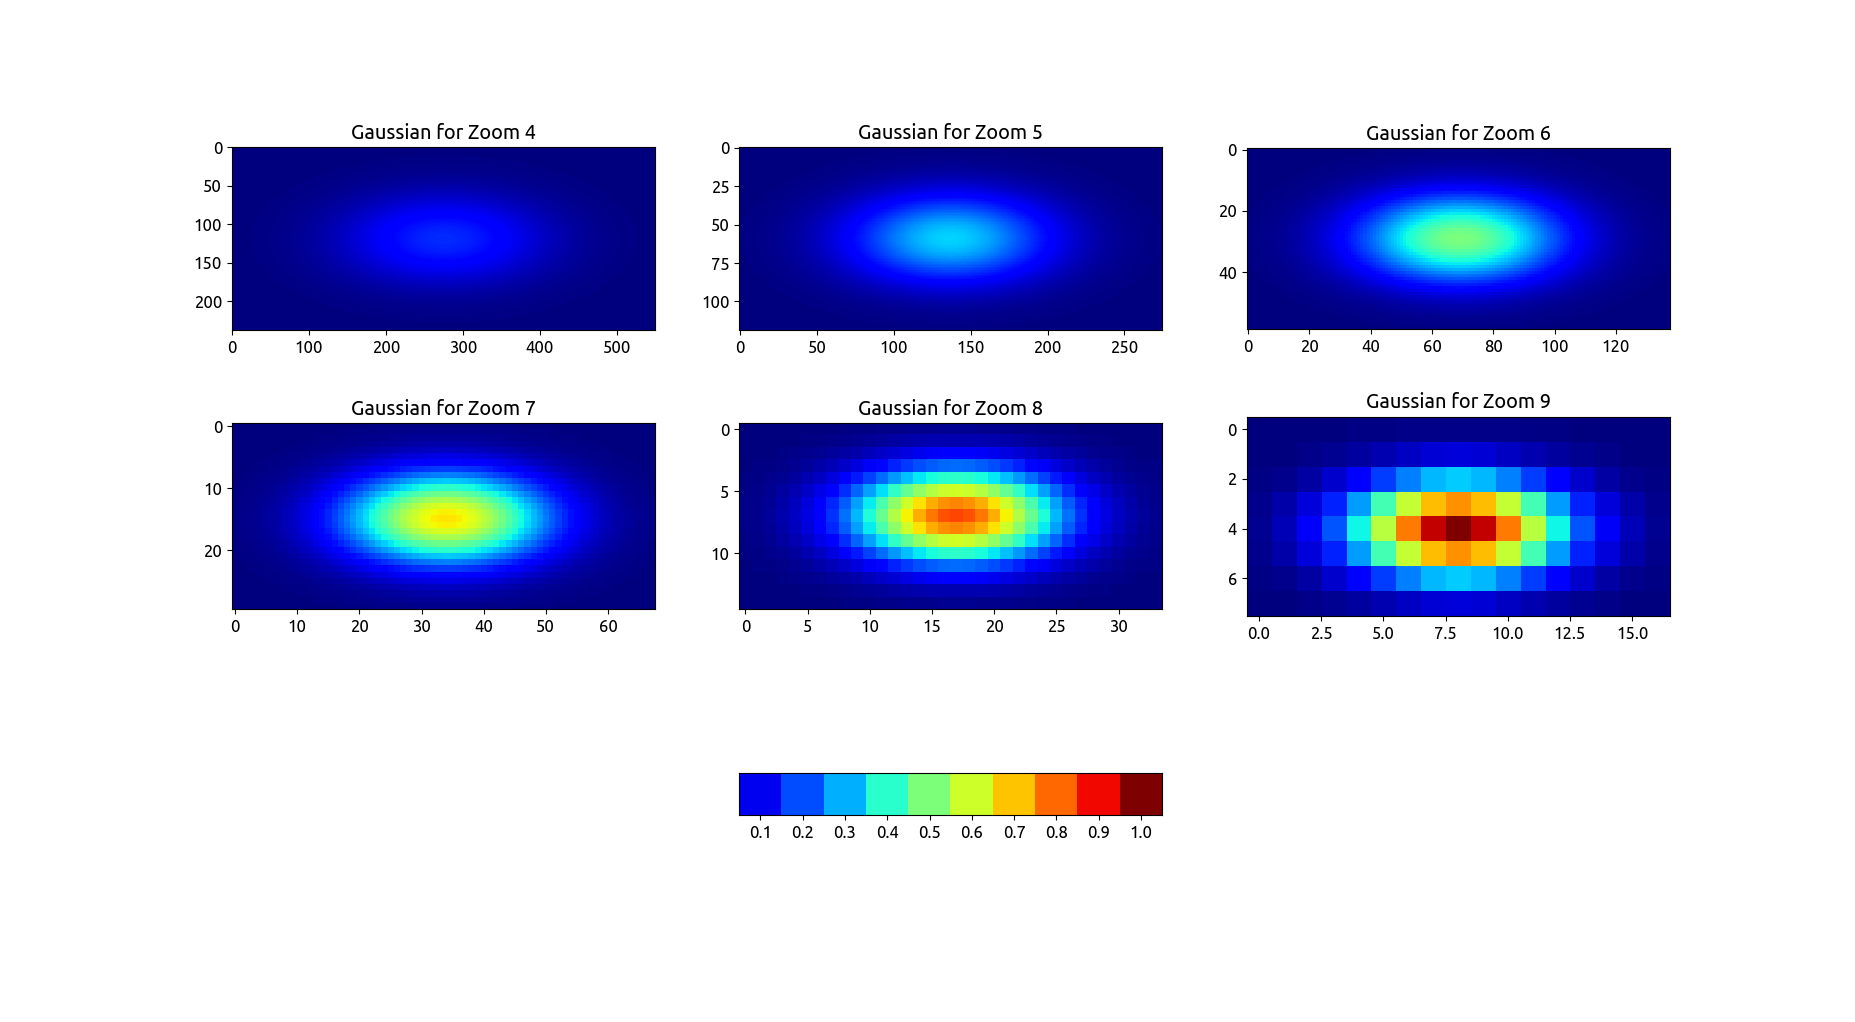
\includegraphics[scale=0.35]{plots/gaussian.png}
\caption{Example Gaussian Grids for an Image that has a zoom up to 9}
\end{center}
\end{figure}

   So each annotation has a center coordinate.
   For this coordinate, a list of Gaussian values is generated based on all the positions near the annotation.
   This vector is sorted inversely.
   It is important to note that it does not take much time for the student to assimilate all the information on a part of an image.
   So the idea is to weight these positions to the point that after enough positions, the next ones would have a weight of close to 0.
To do so, a geometrical sequence was used:
	\[\sum\limits_{i=0}^N w^i\]

N is the number of positions.
In our case, $w$ was set as 0.95.
This means that this sequence converges to 20, and after about 50 positions the sequence is close to the convergence value (about 18).
Since the list of Gaussian values are sorted, the highest values will have the highest weight.
The equation becomes :
	\[score = \sum\limits_{i=0}^N L[i]*w^i\]
With L being the list of Gaussian values for the annotation.
This means that the highest value has a weight of 1, the second a weight of 0.95, the third $0.95*0.95$, and so on.
The value calculated is then used for the score.
If a student actually observed in detail the annotation, they would usually get values above 10.\\

    \item[\textbullet] \textbf{USER SCORE AT IMAGE <x> :} With <x> the image identifier on Cytomine.
    The users are given scores between 0 and 1 (not opening an image gives the user a score of 0).
    The score represents how well the user observed the annotations in the given image.
    In short, if a user spends a good amount of time on top of an annotation or if the user clicks on the annotation, he/she will get points for that annotation.
    Doing so for all annotations gives a final score.
    The score for an annotation is given by the previous variable (SCORE OF ANNOTATION <y> AT IMAGE <x>) and re dimensioned so this variable returns a score between 0 and 1.
    If the image does not have any annotation, the scores for are calculated for the entire image and the average is returned. \\

    \item[\textbullet] \textbf{AVERAGE USER SCORE :} The average of all the scores defined previously for a user. \\

    \item[\textbullet] \textbf{NB POSITIONS AT IMAGE <x> :} with <x> being the image Identifier, represents the number of positions recorded at that image for a user. \\

   \item[\textbullet] \textbf{TIME SPENT AT IMAGE <x> :} With <x> being the image identifier, represents the total time spent on an image for a user. \\

   \item[\textbullet] \textbf{NB OF ANNOTATION ACTIONS AT IMAGE <x> :} With <x> being the image identifier, represents the number of annotation Actions at that image for a user. \\

    \item[\textbullet] \textbf{NB OF POSITIONS WITH ZOOM <y> AT IMAGE <x> :} With <x> being the image identifier and <y> being the zoom value [1-10].
    It Represents the number of positions for a certain zoom  at that image for a user. \\

    \item[\textbullet] \textbf{NB IMAGES VISITED DURING MODULE <x> :} The total number of different images that a user has opened that are associated to the module <x>.\\

    \item[\textbullet] \textbf{AVG NB POSITIONS DURING MODULE <x> :} The mean number of positions obtained relative to all the images opened that are associated to the module <x> during the corresponding time period.\\

    \item[\textbullet] \textbf{MEDIAN NB POSITIONS DURING MODULE <x> :} The median number of positions obtained relative to all the images opened that are associated to the module <x> during the corresponding time period.\\

    \item[\textbullet] \textbf{TOTAL NB POSITIONS DURING MODULE <x> :} The total number of positions obtained from all the images associated to the module <x> during the corresponding time period.\\

    \item[\textbullet] \textbf{TOTAL TIME SPENT DURING MODULE <x> (s) :} Total amount of time spent viewing images associated to the module <x> during its given time period.\\

    \item[\textbullet] \textbf{AVG TIME SPENT DURING MODULE <x> (s) :} Mean amount of time spent viewing images associated to the module <x> during its given time period.\\

    \item[\textbullet] \textbf{MEDIAN TIME SPENT DURING MODULE <x> (s) :} median amount of time spent viewing images associated to the module <x> during its given time period.\\

    \item[\textbullet] \textbf{NB POSITIONS DURING MODULE <y> FOR IMAGE <x> :} with <x> being the image Identifier of an image associated to the module <y>.
    This represents the number of positions recorded at that image for a user during the module's time period. \\

    \item[\textbullet] \textbf{TIME SPENT DURING MODULE <y> FOR IMAGE <x> :} with <x> being the image Identifier of an image associated to the module <y>.
    This represents the time spent at that image for a user during the module's time period. \\

    \item[\textbullet] \textbf{NB ANNOTATION ACTIONS DURING MODULE <y> FOR IMAGE <x> :} with <x> being the image Identifier of an image associated to the module <y>.
    This represents the number of annotation actions recorded at that image for a user during the module's time period. \\


     \item[\textbullet] \textbf{NB POSITIONS WITH ZOOM <z> DURING MODULE <y> AT IMAGE <x> :} with <x> being the image Identifier of an image associated to the module <y>.
     This represents the number of positions recorded at that image for a user during the module's time period with zoom <z>.
     The zoom value <z> ranges from 1 to 10. \\

     \item[\textbullet] \textbf{AVERAGE ZOOM DURING MODULE <y> FOR IMAGE <x> :} with <x> being the image Identifier of an image associated to the module <y>.
     This represents the average zoom level of all the positions recorded at that image for a user during the module's time period. \\

     \item[\textbullet] \textbf{MEDIAN ZOOM DURING MODULE <y> FOR IMAGE <x> :} with <x> being the image Identifier of an image associated to the module <y>.
     This represents the median zoom level of all the positions recorded at that image for a user during the module's time period. \\

     \item[\textbullet] \textbf{NB POSITIONS AT ZOOM <z> DURING MODULE <x> :} with <z> between 1 and 10, calculated for all the images associated to the module <x>.
     This represents the number of positions for a specific zoom for a user during the module's time period. \\

	\item[\textbullet] \textbf{AVERAGE NB POSITIONS AT ZOOM <z> DURING MODULE <x> :} with <z> between 1 and 10, calculated for all the images associated to the module <x>.
	This represents the mean number of positions for a specific zoom for a user during the module's time period. \\

	\item[\textbullet] \textbf{MEDIAN NB POSITIONS AT ZOOM <z> DURING MODULE <x> :} with <z> between 1 and 10, calculated for all the images associated to the module <x>.
	This represents the median number of positions for a specific zoom for
a user during the module's time period. \\

	\item[\textbullet] \textbf{TOTAL NB ANNOTATION ACTIONS DURING MODULE <x> :} With <x> being the module identifier, it represents the total number of annotation  actions for a user during the module's time period. \\

	\item[\textbullet] \textbf{AVG NB ANNOTATION ACTIONS DURING MODULE <x> :} With <x> being the module identifier, it represents the mean number of annotation  actions for a user during the module's time period. \\

	\item[\textbullet] \textbf{MEDIAN NB ANNOTATION ACTIONS DURING MODULE <x> :} With <x> being the module identifier, it represents the median number of annotation  actions for a user during the module's time period. \\

	\item[\textbullet] \textbf{AVERAGE USER SCORE DURING MODULE <x> :} With <x> being the module identifier, it represents the average predefined score for a user for the module's images during the respective time period. \\

	\item[\textbullet] \textbf{USER SCORE AT IMAGE <y> DURING MODULE <x> :} With <x> being the module identifier and <y> the image identifier, it represents the predefined score at the image for a user during the module's time period. \\

	\item[\textbullet] \textbf{SCORE OF ANNOTATION <z> AT IMAGE <y> DURING MODULE <x> :} With <x> being the module identifier and <y> the image identifier, it represents the predefined score of the annotation <z> at the image for a user during the module's time period. \\

    \item[\textbullet] \textbf{PERCENT TIME WORKED AT NIGHT :} Value from 0 to 1.
    This represents the ratio of the time spent working from 6pm to 6am.

    \item[\textbullet] \textbf{PERCENT TIME WORKED LATE :} Value from 0 to 1.
    This represents the ratio of the time spent working from 1am to 6am.

    \item[\textbullet] \textbf{PERCENT TIME WORKED MORNING :} Value from 0 to 1.
    This represents the ratio of the time spent working from 6am to 12pm.

    \item[\textbullet] \textbf{NUMBER OF DAYS WORKED :} The total number of days where a user opened at least one image.

    \item[\textbullet] \textbf{PERCENT TIME WORKED DURING MODULE <x> :} When working on Cytomine, the user can open images associated during a module during its time period or outside of it.
    This represents the ratio of the user activity during the time period.

	\item[\textbullet] \textbf{ANNOTATION <y> VISITED BEFORE ANNOTATION <y + 1> AT IMAGE <X> :} This binary variable determines whether or not a student visited the annotation <y> before the annotation <y + 1> for an image <x>.
	The users are encouraged to study the reference annotation in a specific order.

    \end{itemize}


    All these features end up describing how users participated on Cytomine and their effects will be analyzed.
    It will be evident that most of these features will have little impact in the learning process.

    \section{Results}

    \subsection{Comparing Timelines}

        In this small experiment, there were a total of 8 timelines generated.
        Four of those belonging to the students with the highest grades and four belonging to the students with the lowest grades.
        The simple objective is to compare the results from the two sets and also compare results within a set. (Figures \ref{fig:tm1} and \ref{fig:tm2})

      \begin{figure}[H]
      \centering
  	  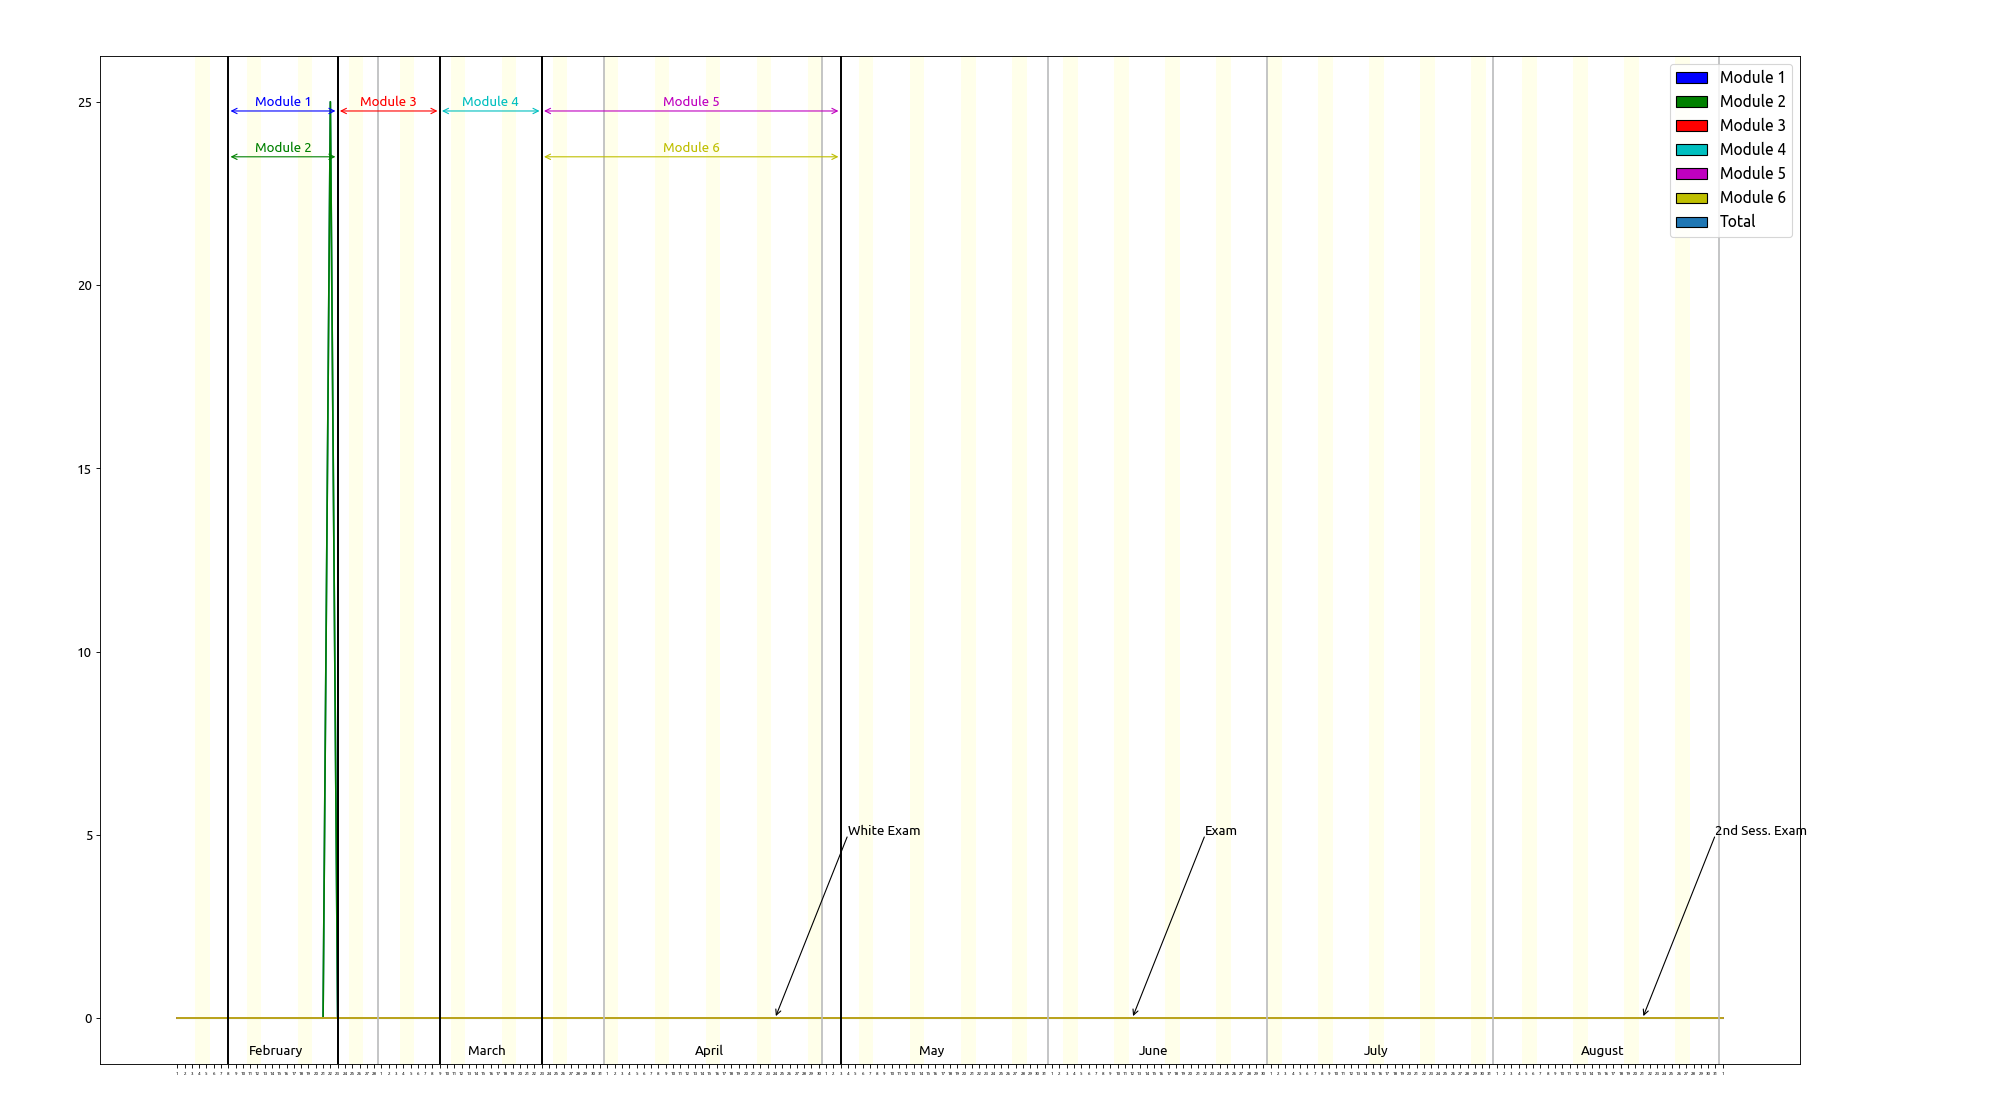
\includegraphics[width=.48\linewidth]{images/bad_timeline_7110523.png}
  	  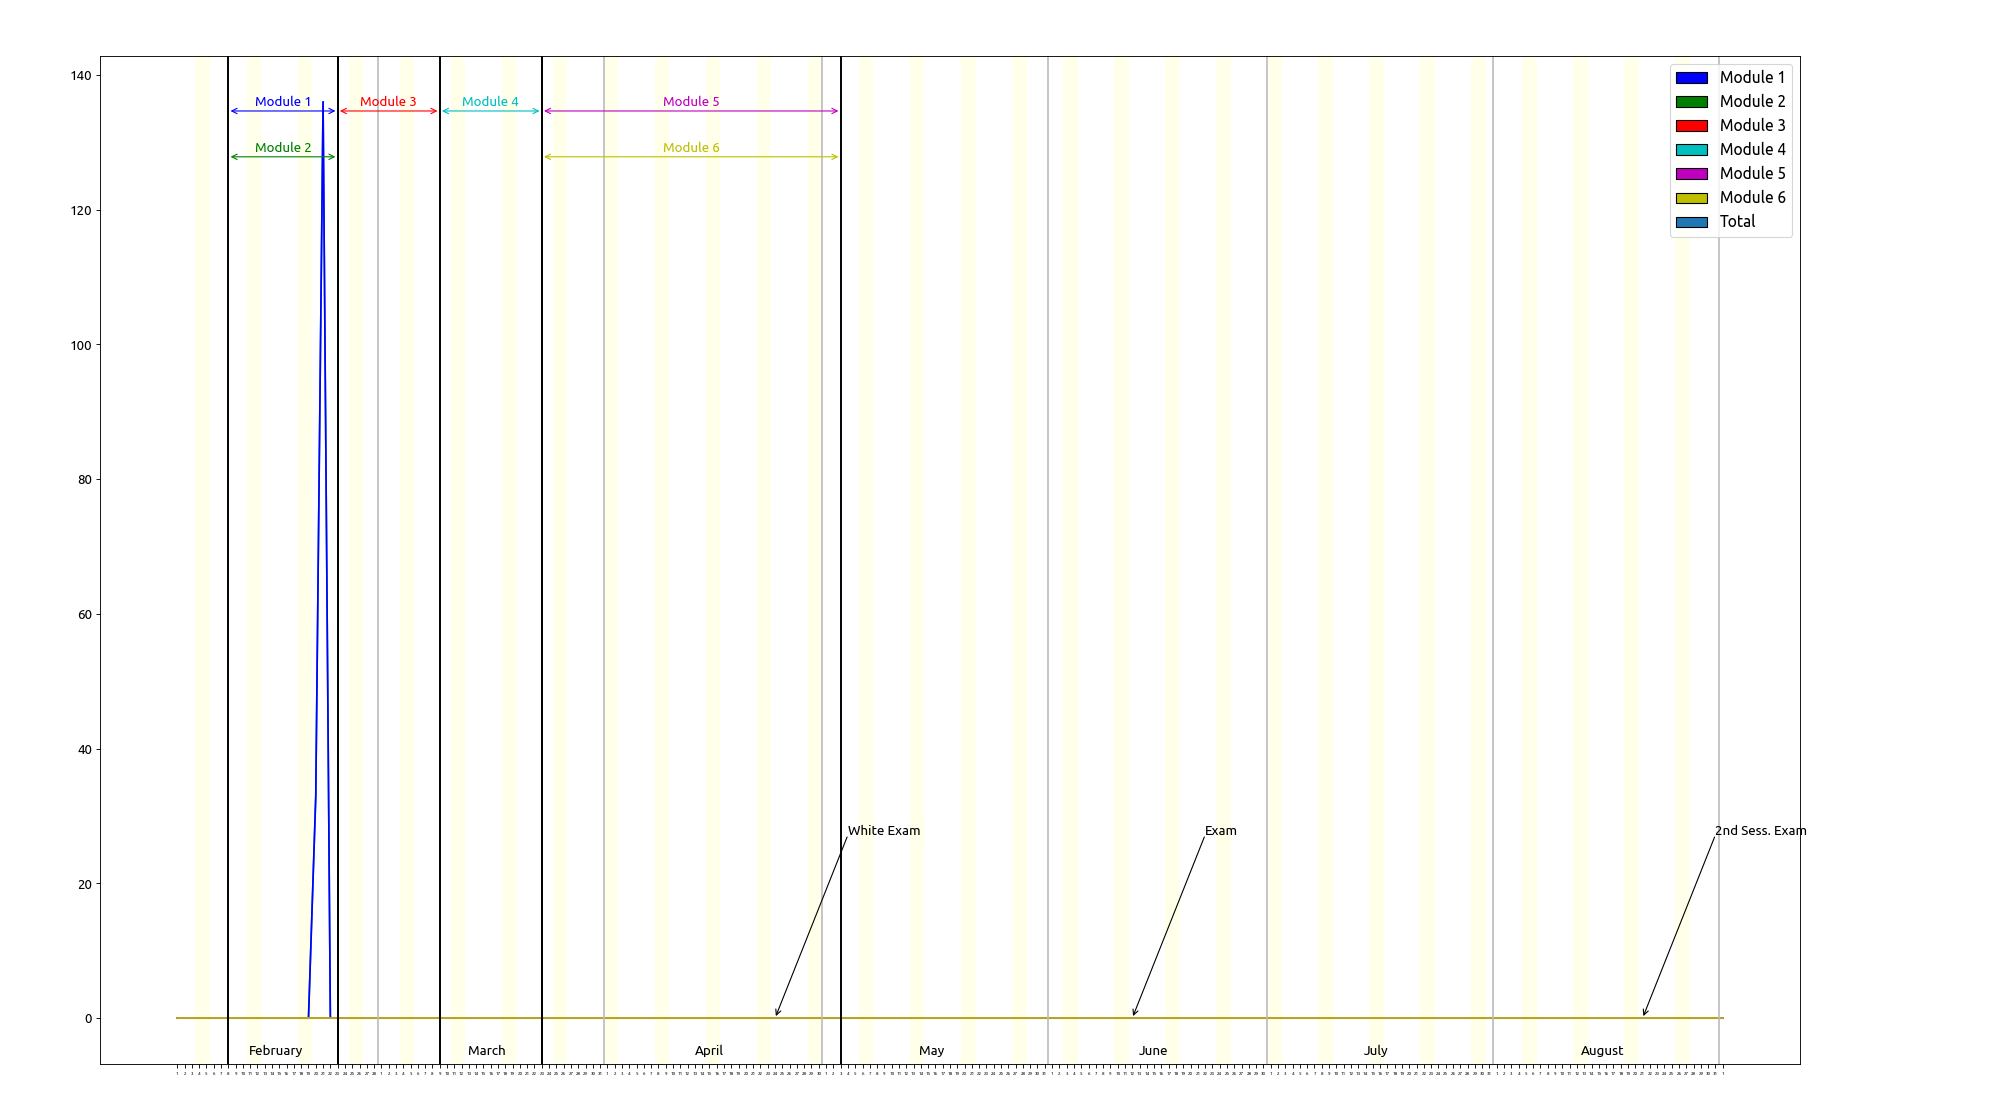
\includegraphics[width=.48\linewidth]{images/bad_timeline_6370413.png}
      \\
      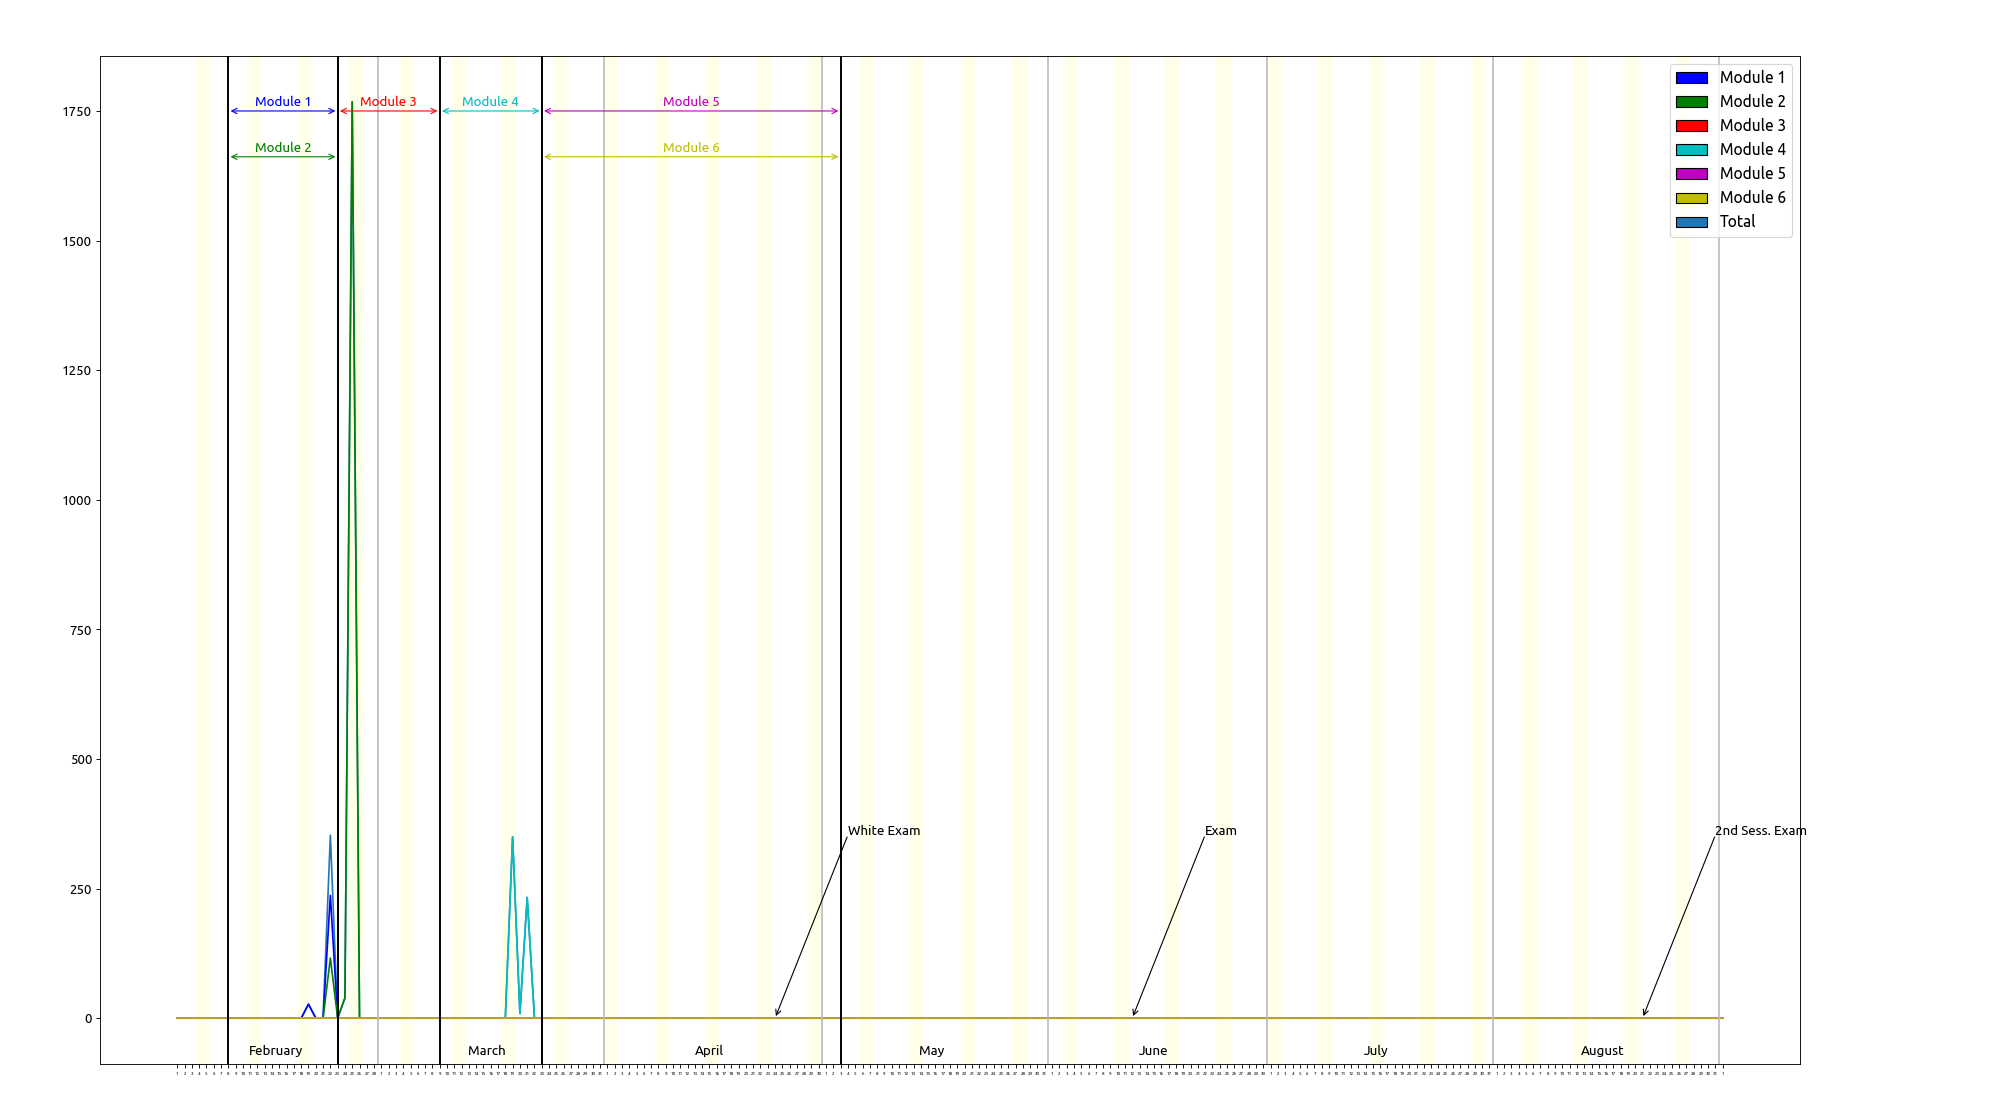
\includegraphics[width=.48\linewidth]{images/bad_timeline_5897419.png}
      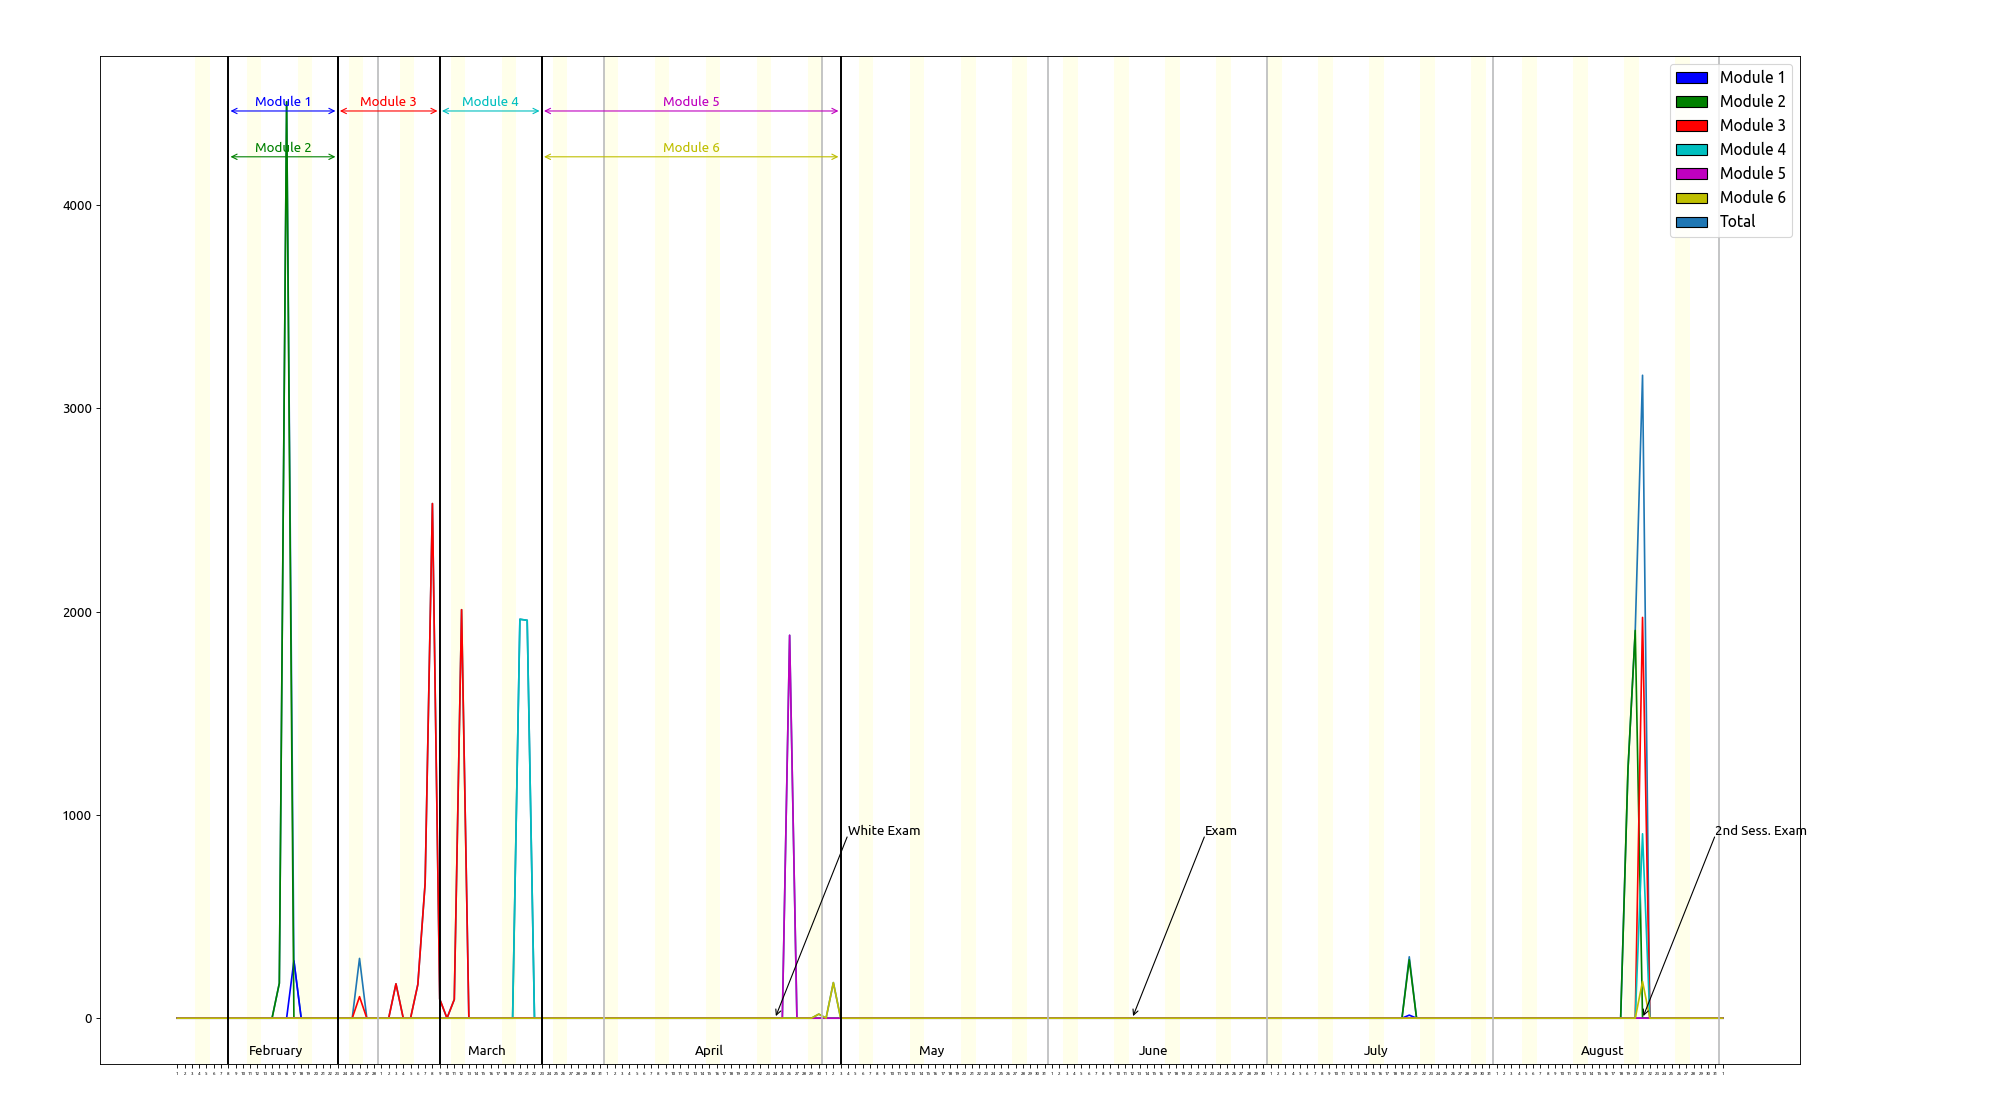
\includegraphics[width=.48\linewidth]{images/bad_timeline_3905979.png}
      \caption{Timelines of the students with the lowest grades}
      \label{fig:tm1}
      \end{figure}


      \begin{figure}[H]
      \centering
  	  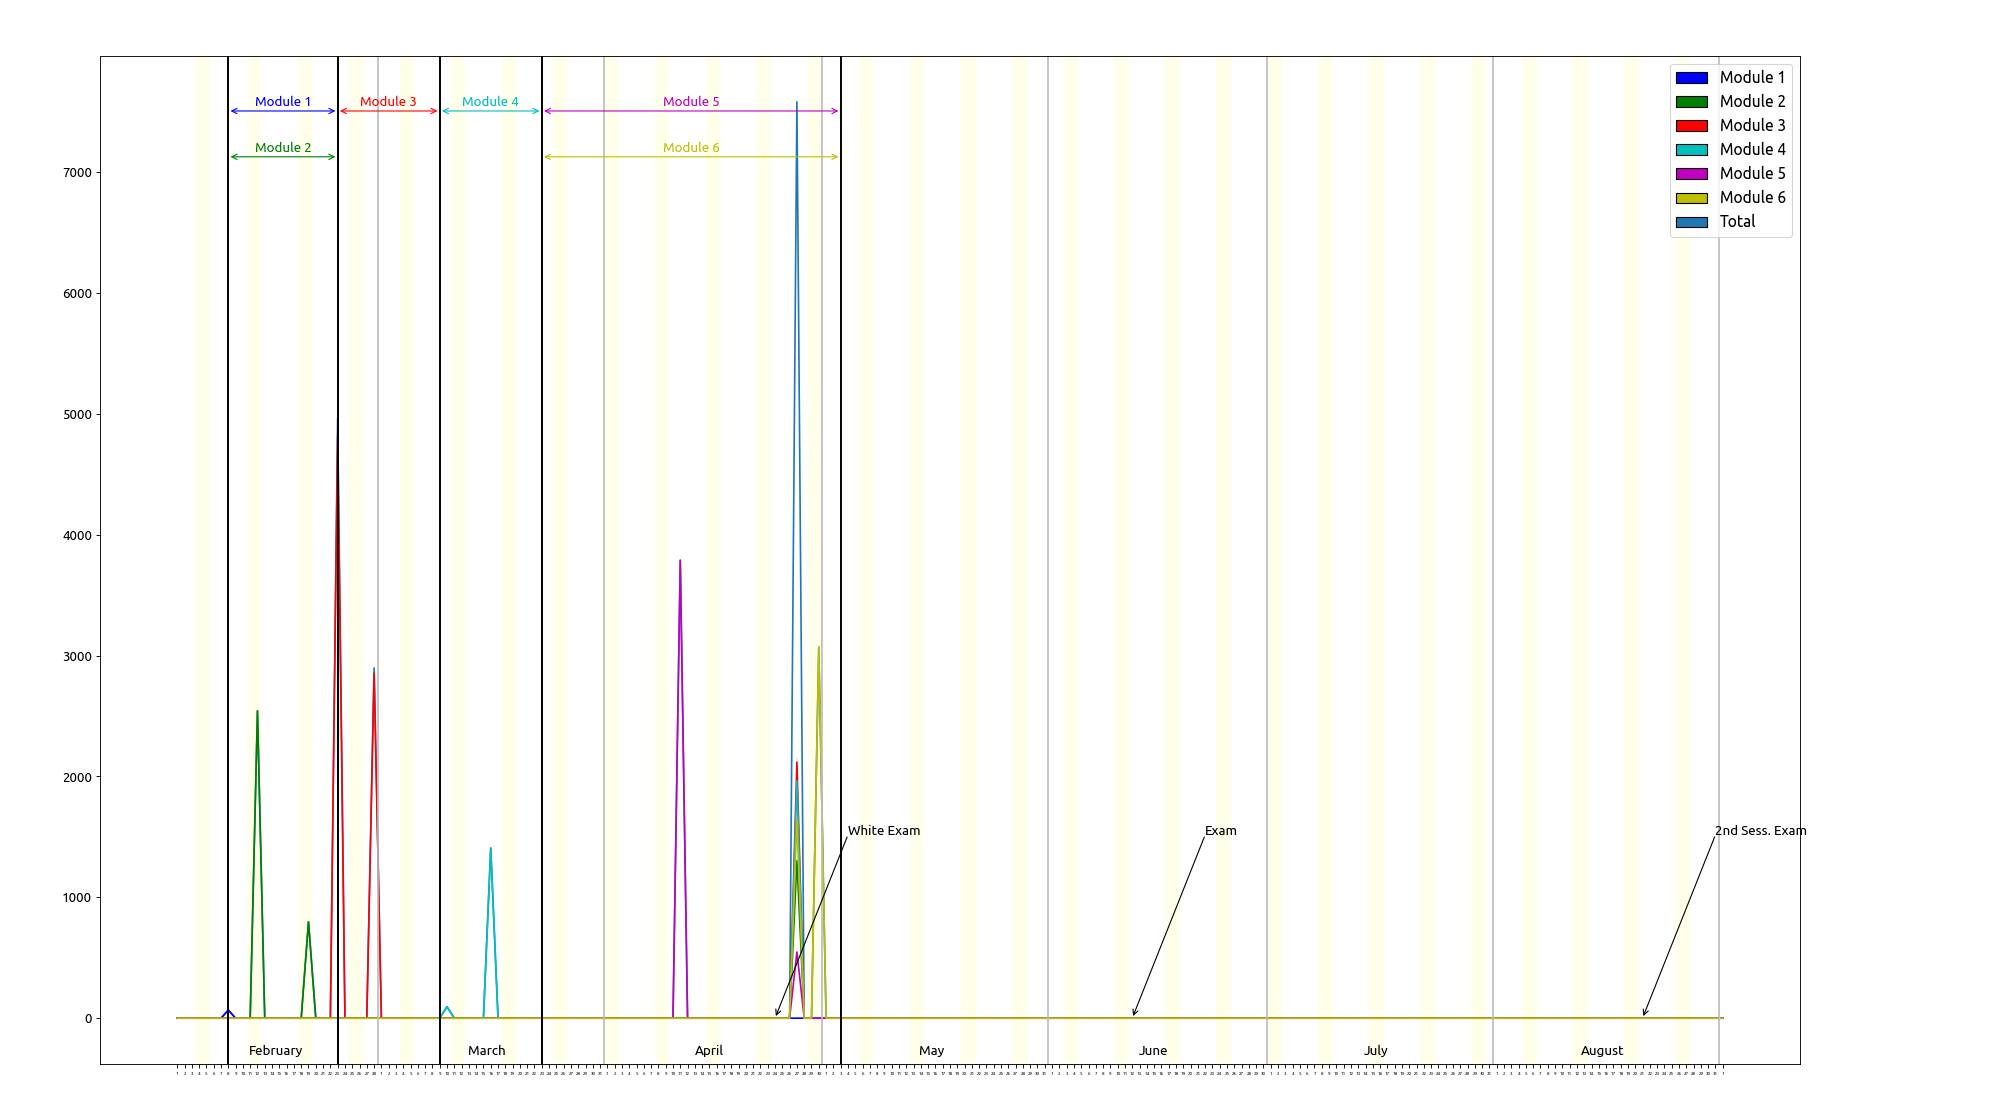
\includegraphics[width=.48\linewidth]{images/good_timeline_1747564.png}
  	  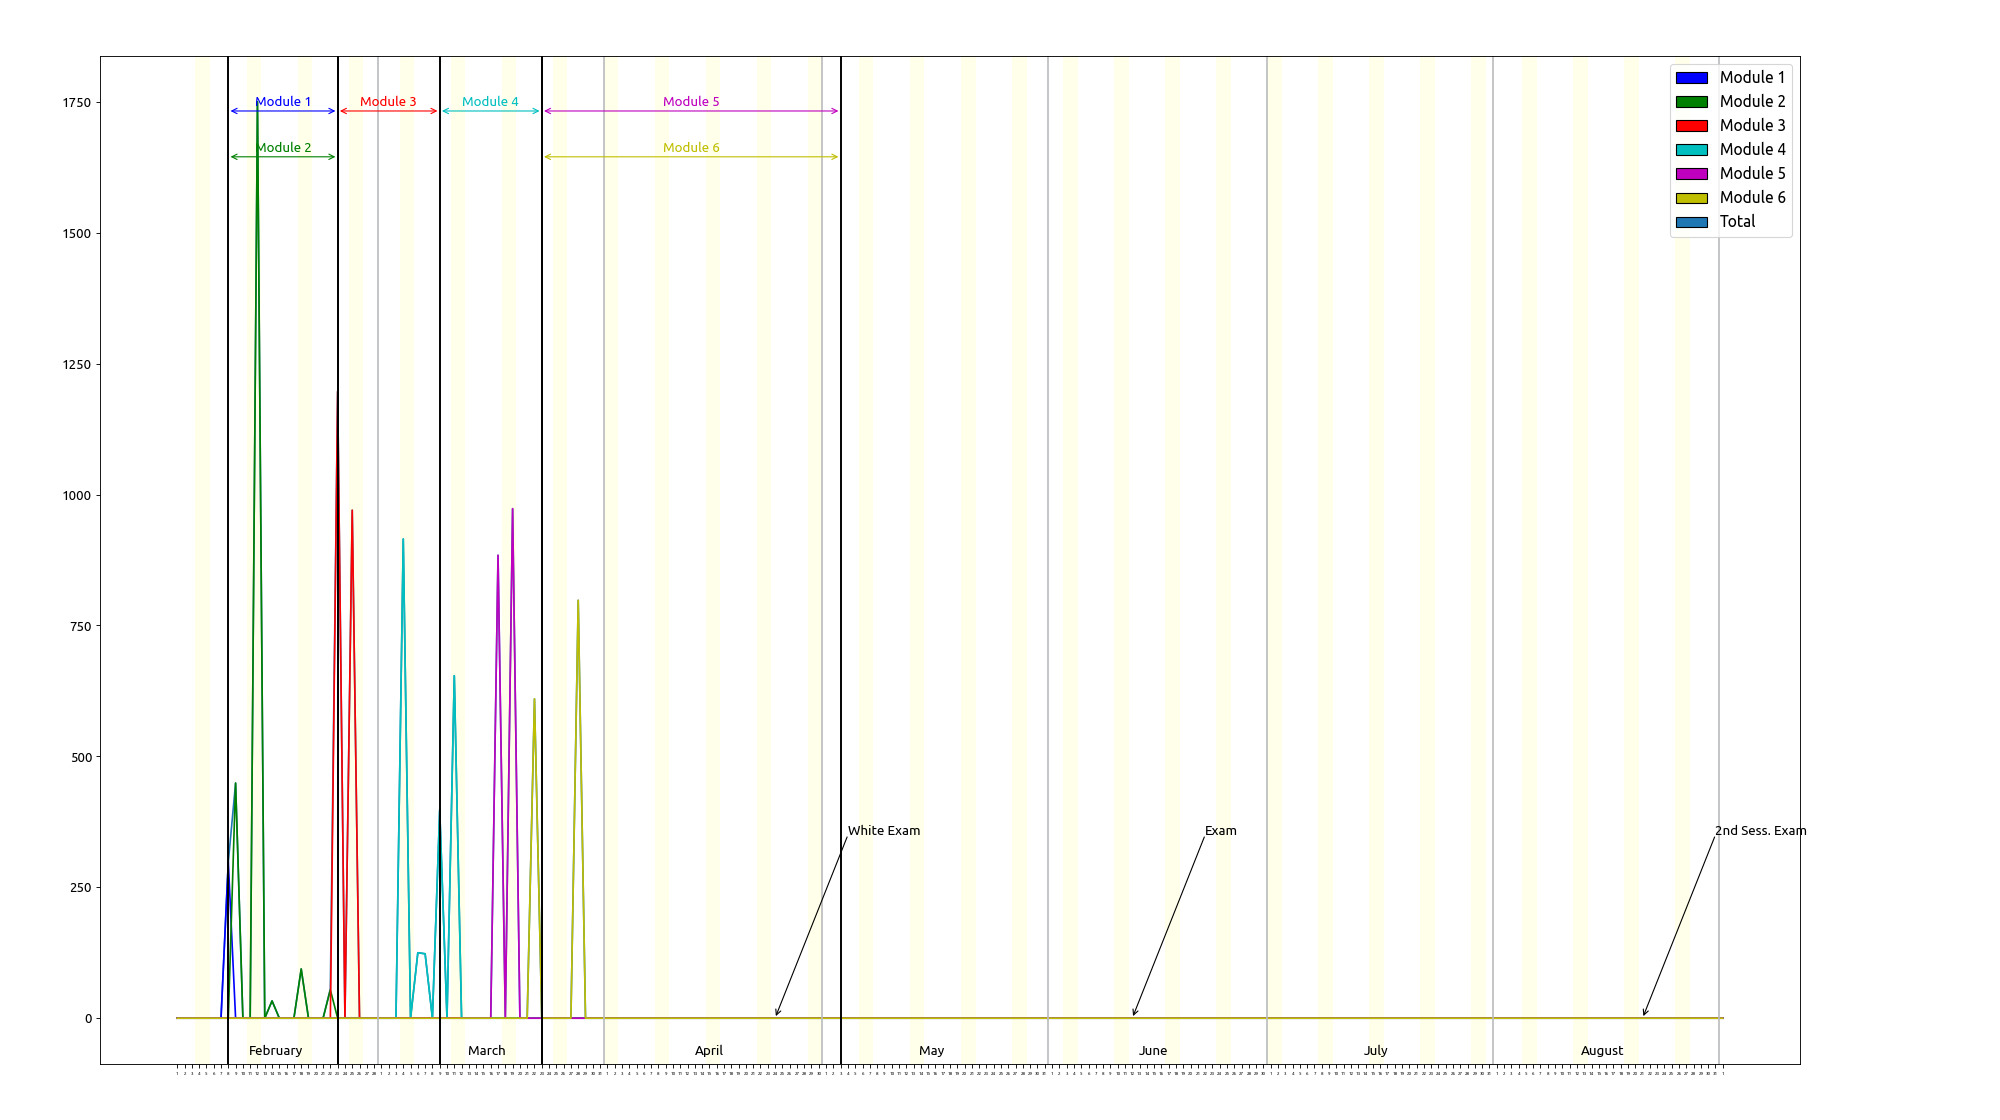
\includegraphics[width=.48\linewidth]{images/good_timeline_1793969.png}
      \\
      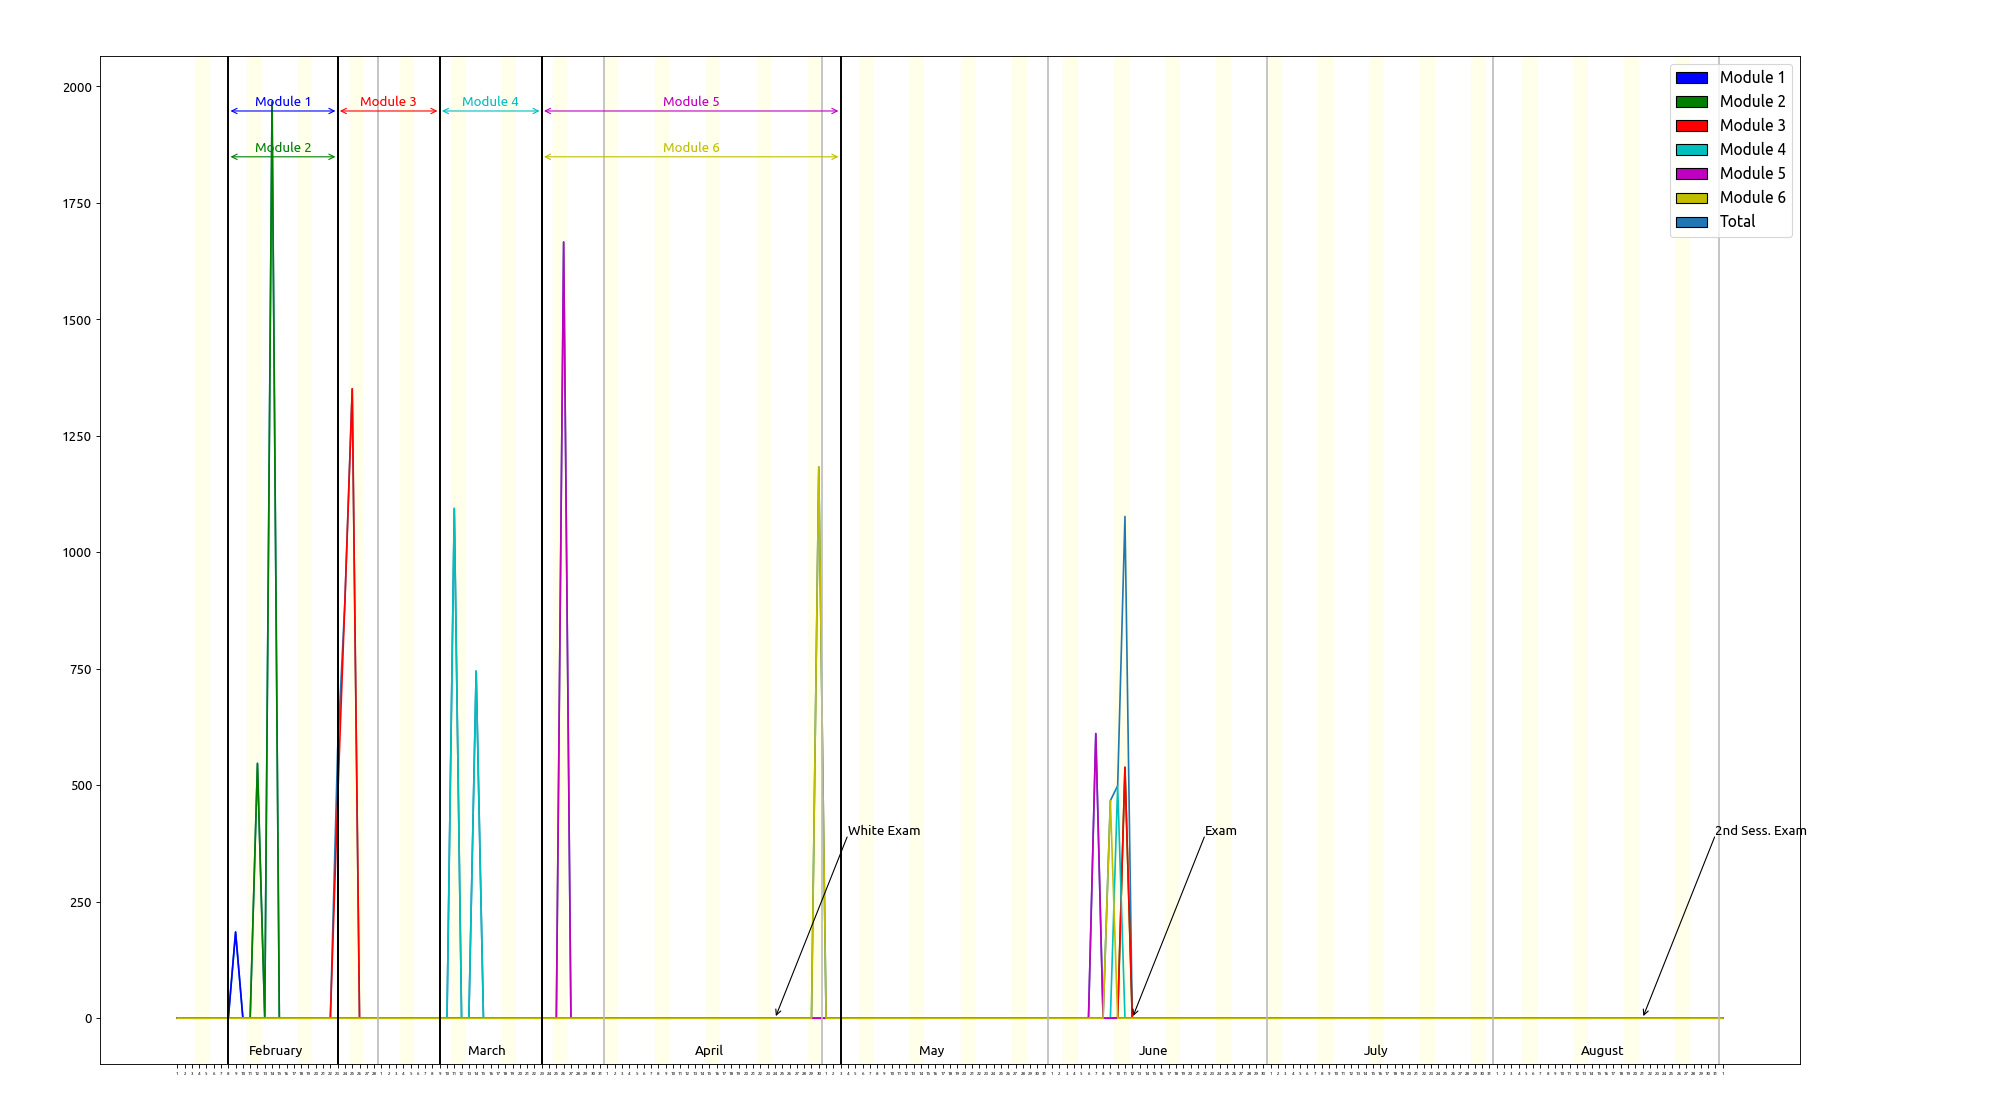
\includegraphics[width=.48\linewidth]{images/good_timeline_1942114.png}
      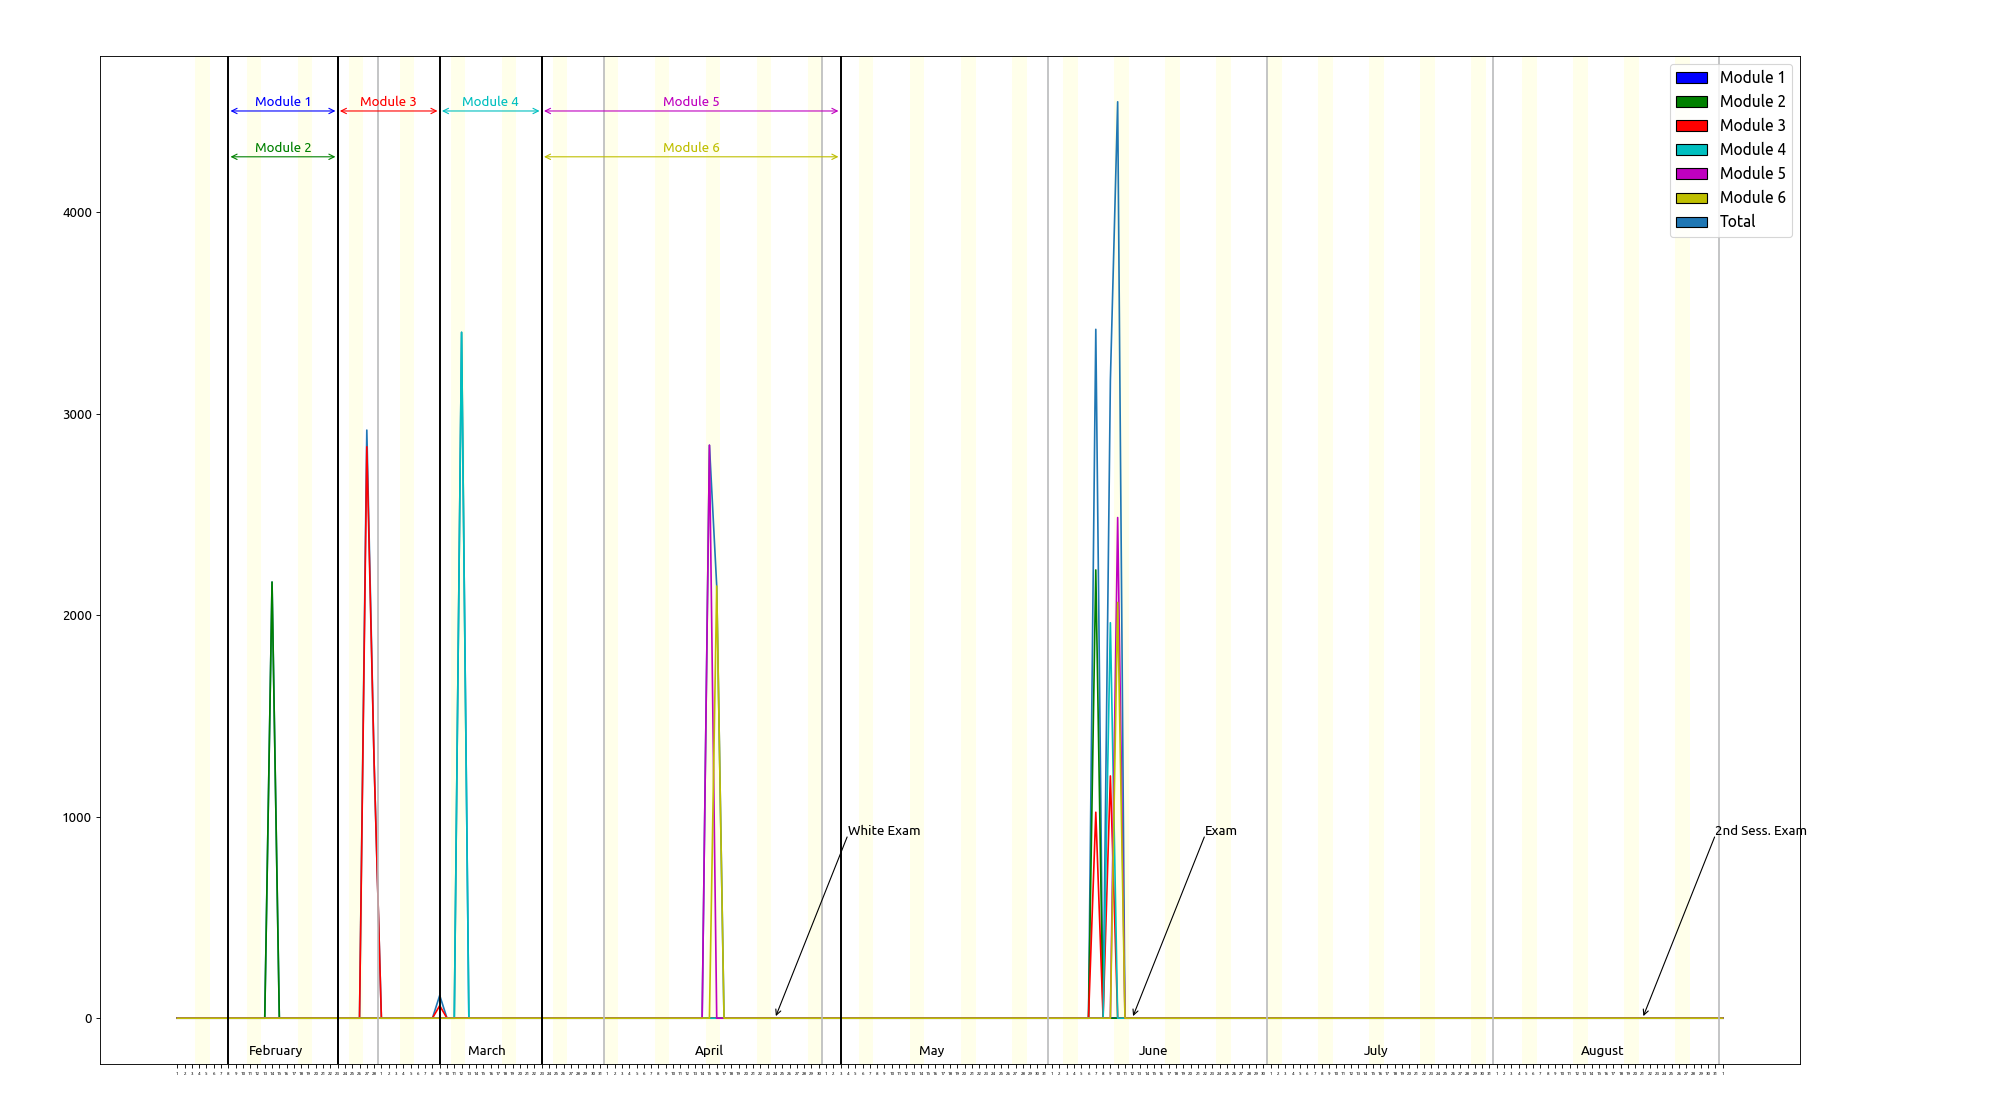
\includegraphics[width=.48\linewidth]{images/good_timeline_3554348.png}
      \caption{Timelines of the students with the highest grades}
      \label{fig:tm2}
      \end{figure}

    For the timelines of students with the lowest grades, for the most part it is pretty straightforward.
    There are are a small number of positions and some modules were not even visited.
    There is one student who followed different patterns with a respectable activity.
    Unfortunately, the student still failed the exam.\\

    Meanwhile, for the students with th highest grades, there are many more positions as a whole.
    Also, images for all the modules were visited.
    There is a clear difference between the two sets.
    But in the set of students with the highest grades, there are many different patterns.
    Some students have a significant higher activity than others.
    One worked on modules ahead of time, and some didn't even log onto Cytomine the weeks before the exam.
    This shows that it is hard to judge a student's performance and comprehension of the course.
    Students follow different habbits and exhibit different patterns.
    There is no "best" method for studying according to this small study.
    The Machine Learning can give more insight on this question.



    \subsection{White Test Grades}

    These 3 ungraded exams were taken halfway during the semester (24th of April 2017).
    They reflect what a student has learned and remembered up until that day.
    At that point, students should have finished modules 1 through 4 and at least looked at modules 5 and 6.
    These tests could be a great indicator on how well students can perform during the real exam.
    These \textbf{Y} variables were tested using a Leave-one-out cross validation on an Extra Tree Regressor with the generated data set.
    As a reminder, scores are calculated with the Mean Absolute Error technique.
    Also, the results are also compared with a model that learns by simply using the median.
    This is to determine if the model has much merit. (Figure \ref{fig:results_white})
    \begin{figure}[H]
      \centering
  	  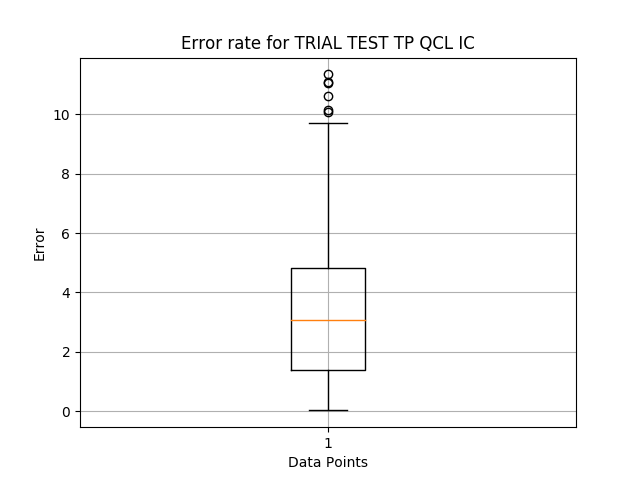
\includegraphics[width=.3\linewidth]{plots/cv_boxplot_TRIAL_TEST_TP_QCL_IC_2018-04-27_14_35_12.png}
  	  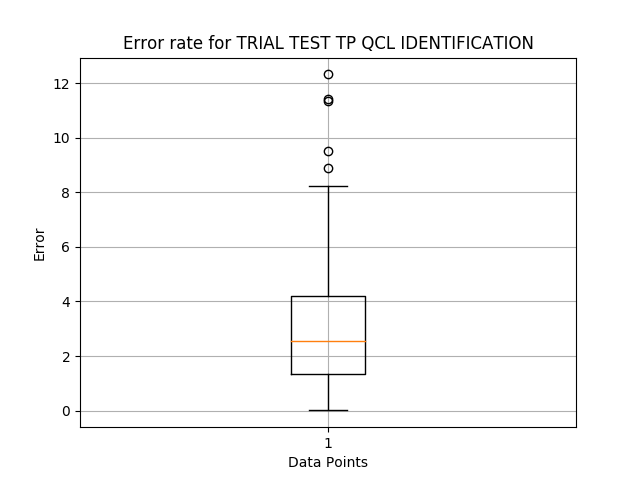
\includegraphics[width=.3\linewidth]{plots/cv_boxplot_TRIAL_TEST_TP_QCL_IDENTIFICATION_2018-04-27_14_31_56.png}
      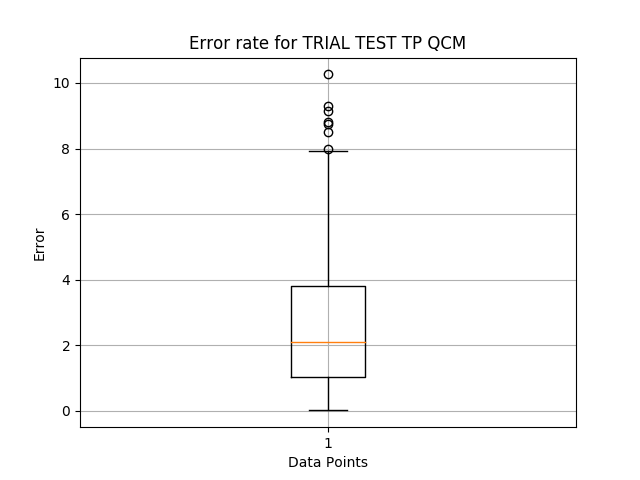
\includegraphics[width=.3\linewidth]{plots/cv_boxplot_TRIAL_TEST_TP_QCM_2018-04-27_17_16_59.png}
      \\
      \ref{fig:results_white}.1: Boxplots of the error values
      \\
      \vspace{0.5cm}
      \begin{tabular}{| l | c | c | c | c | c |}
      \hline
      & \tiny{Score} & \tiny{Median Score} & \tiny{Score Difference} & \tiny{Real Median Grade} & \tiny{Median Est.
      Grade}\\ \hline
      \tiny{QCL incidence white test} & \tiny{3.40} & \tiny{3.36} & \tiny{-0.04} & \tiny{13.33} & \tiny{12.45}\\ \hline
      \tiny{QCL identification white test} & \tiny{2.93} & \tiny{3.10} & \tiny{0.16} & \tiny{8.0} & \tiny{8.22}\\ \hline
      \tiny{Practical QCM white test} & \tiny{2.58} & \tiny{2.57} & \tiny{-0.006} & \tiny{10.36} & \tiny{10.27}\\
      \hline
      \end{tabular}\\
      \vspace{0.5cm}
      \ref{fig:results_white}.2: Discrete Results\\
      \vspace{0.3cm}
      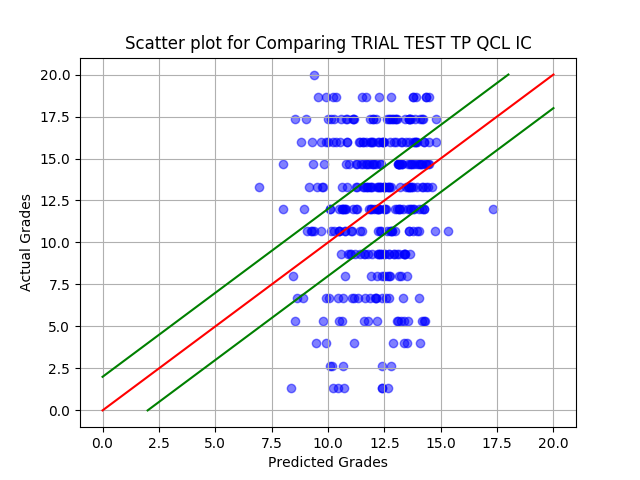
\includegraphics[width=.3\linewidth]{plots/cv_comp_TRIAL_TEST_TP_QCL_IC_2018-04-27_14_35_12.png}
  	  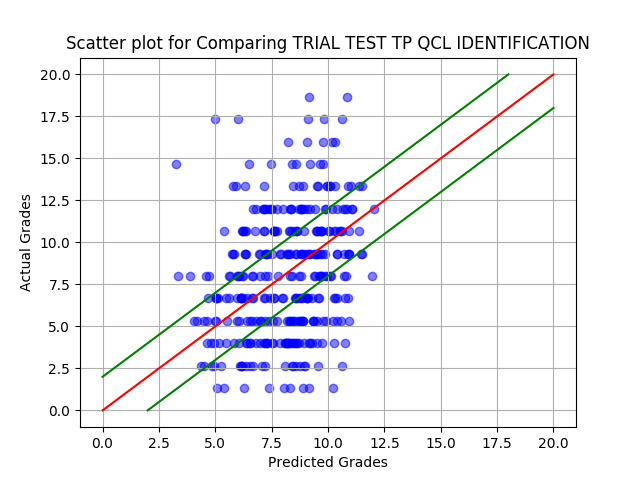
\includegraphics[width=.3\linewidth]{plots/cv_comp_TRIAL_TEST_TP_QCL_IDENTIFICATION_2018-04-27_14_31_55.png}
      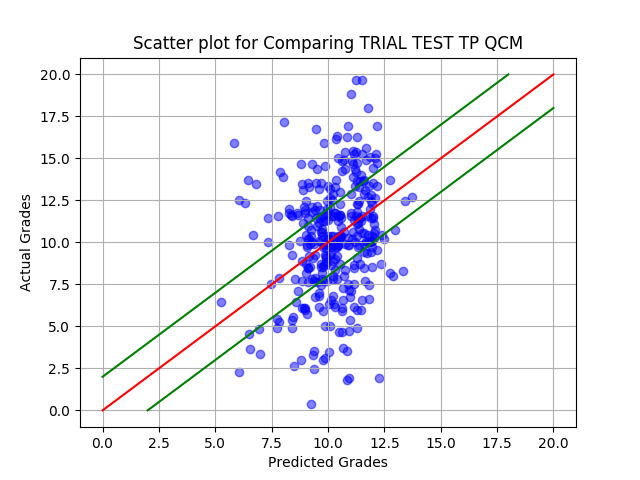
\includegraphics[width=.3\linewidth]{plots/cv_comp_TRIAL_TEST_TP_QCM_2018-04-27_17_16_59.png}
      \\
      \ref{fig:results_white}.3: Actual grades compared to Predicated grades
      \caption{Results from cross-validation of the White Tests}
      \label{fig:results_white}
    \end{figure}

    Unfortunately, the results are not great.
    The boxplots show very high median and quartiles.
    There are also a high number of extreme errors with some above 10.
    The scores represent the average error of the cross validation.
    With scores nearing nearing 3, in some cases, it is better to try and guess using the median value.
    For the incidence test, it seems that the scores are underestimated, this seems to be the case because there is a significantly high grades compared to low grades.
    There are many reasons why results are the way they are.
    This includes the fact that these grades do not rely on activity that occur after the exam date.
    When comparing grade the learned grades against the original grades, it is noticeable that the estimated grades tend to predict values close to the average of the actual grades.
    This makes it so that high and low actual grades when predicted tend to be more erroneous.
    The sample also lacks a good amount of extreme grades which gives the algorithm less to work with for these cases.
    Furthermore, the fact that the exams are ungraded puts less pressure on the students to succeed.
    Therefore, they might not take the tests as seriously as they could by not reviewing and studying the days before. (see Figure \ref{fig:timelapse}) \\


  Since the models are made using regression trees, it it possible to study the features that had an impact in determining the predicted grades.
  Even though the results were not ideal, it is interesting to observe what images and variables had a big impact on determining the grades.
  These images can very well be the subject of a question on the exam. (Figures \ref{fig:var_white1}, \ref{fig:var_white2}, \ref{fig:var_white3})

     \begin{figure}[H]
      \centering
      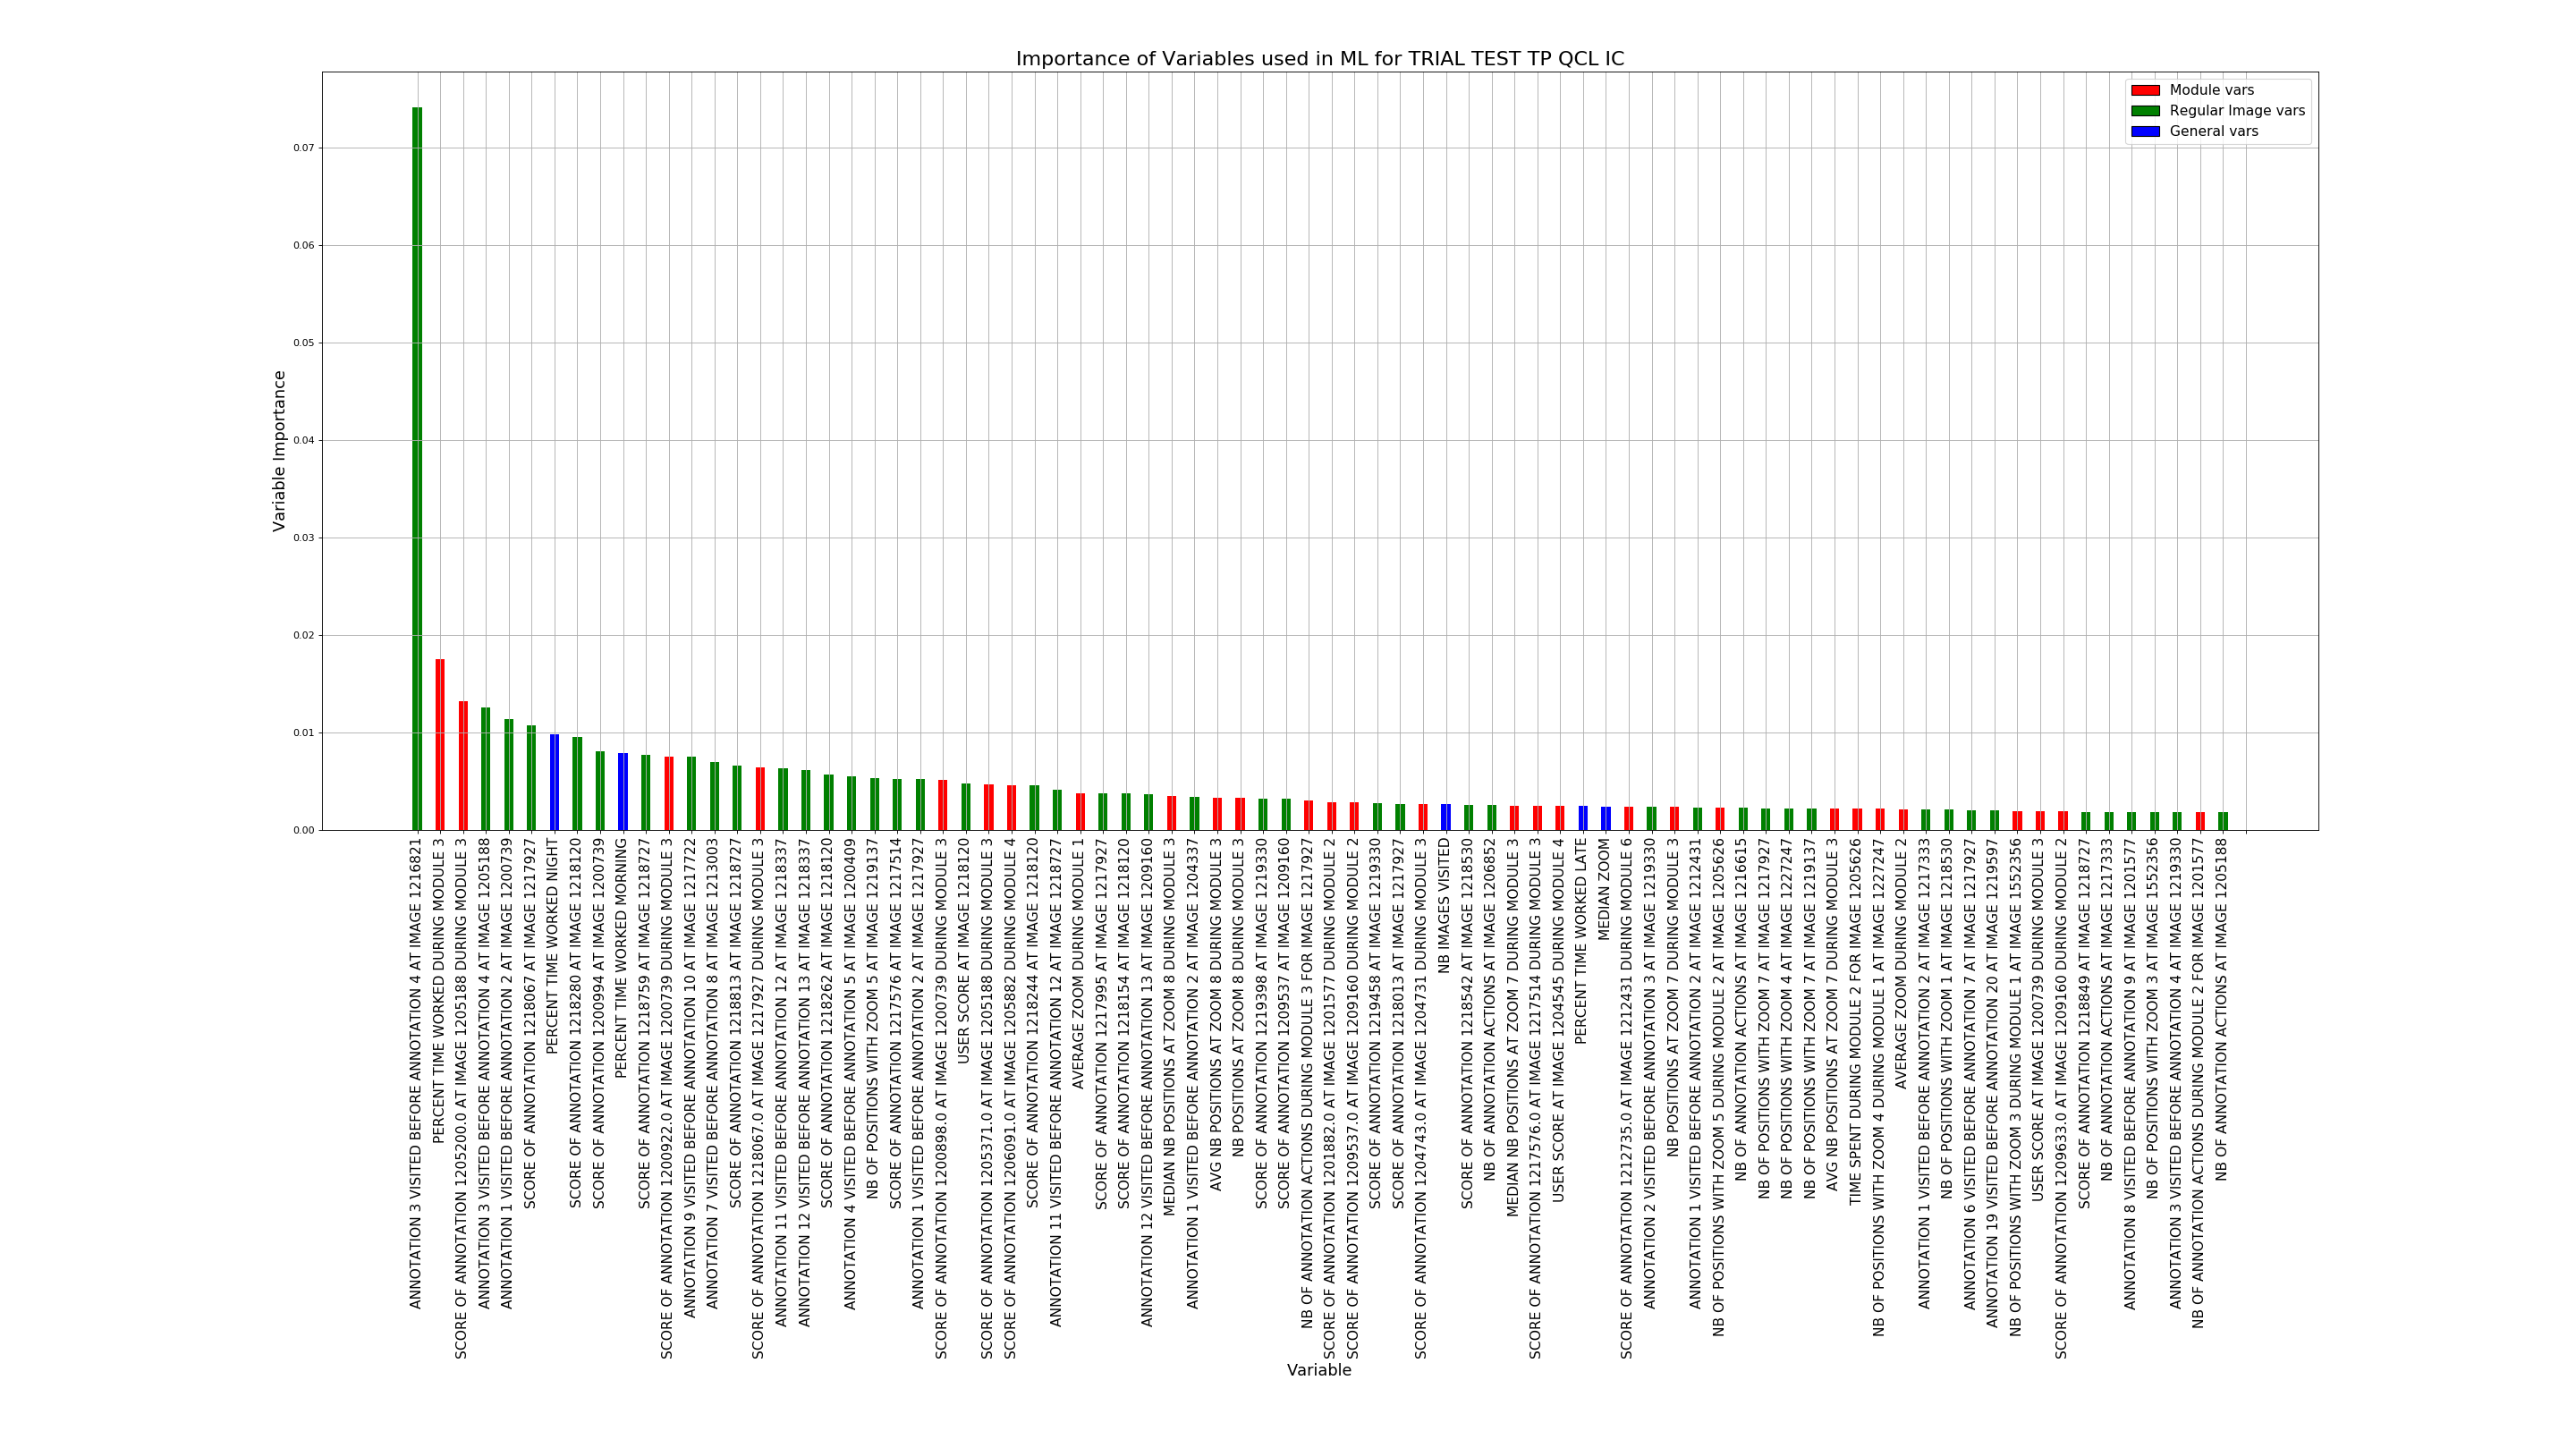
\includegraphics[width=.99\linewidth]{plots/var_importance_TRIAL_TEST_TP_QCL_IC_2018-04-29_14_31_17.png}
      \caption{Feature Importance for QCL the Incidence}
      \label{fig:var_white1}
      \end{figure}

      \begin{figure}[H]
      \centering
      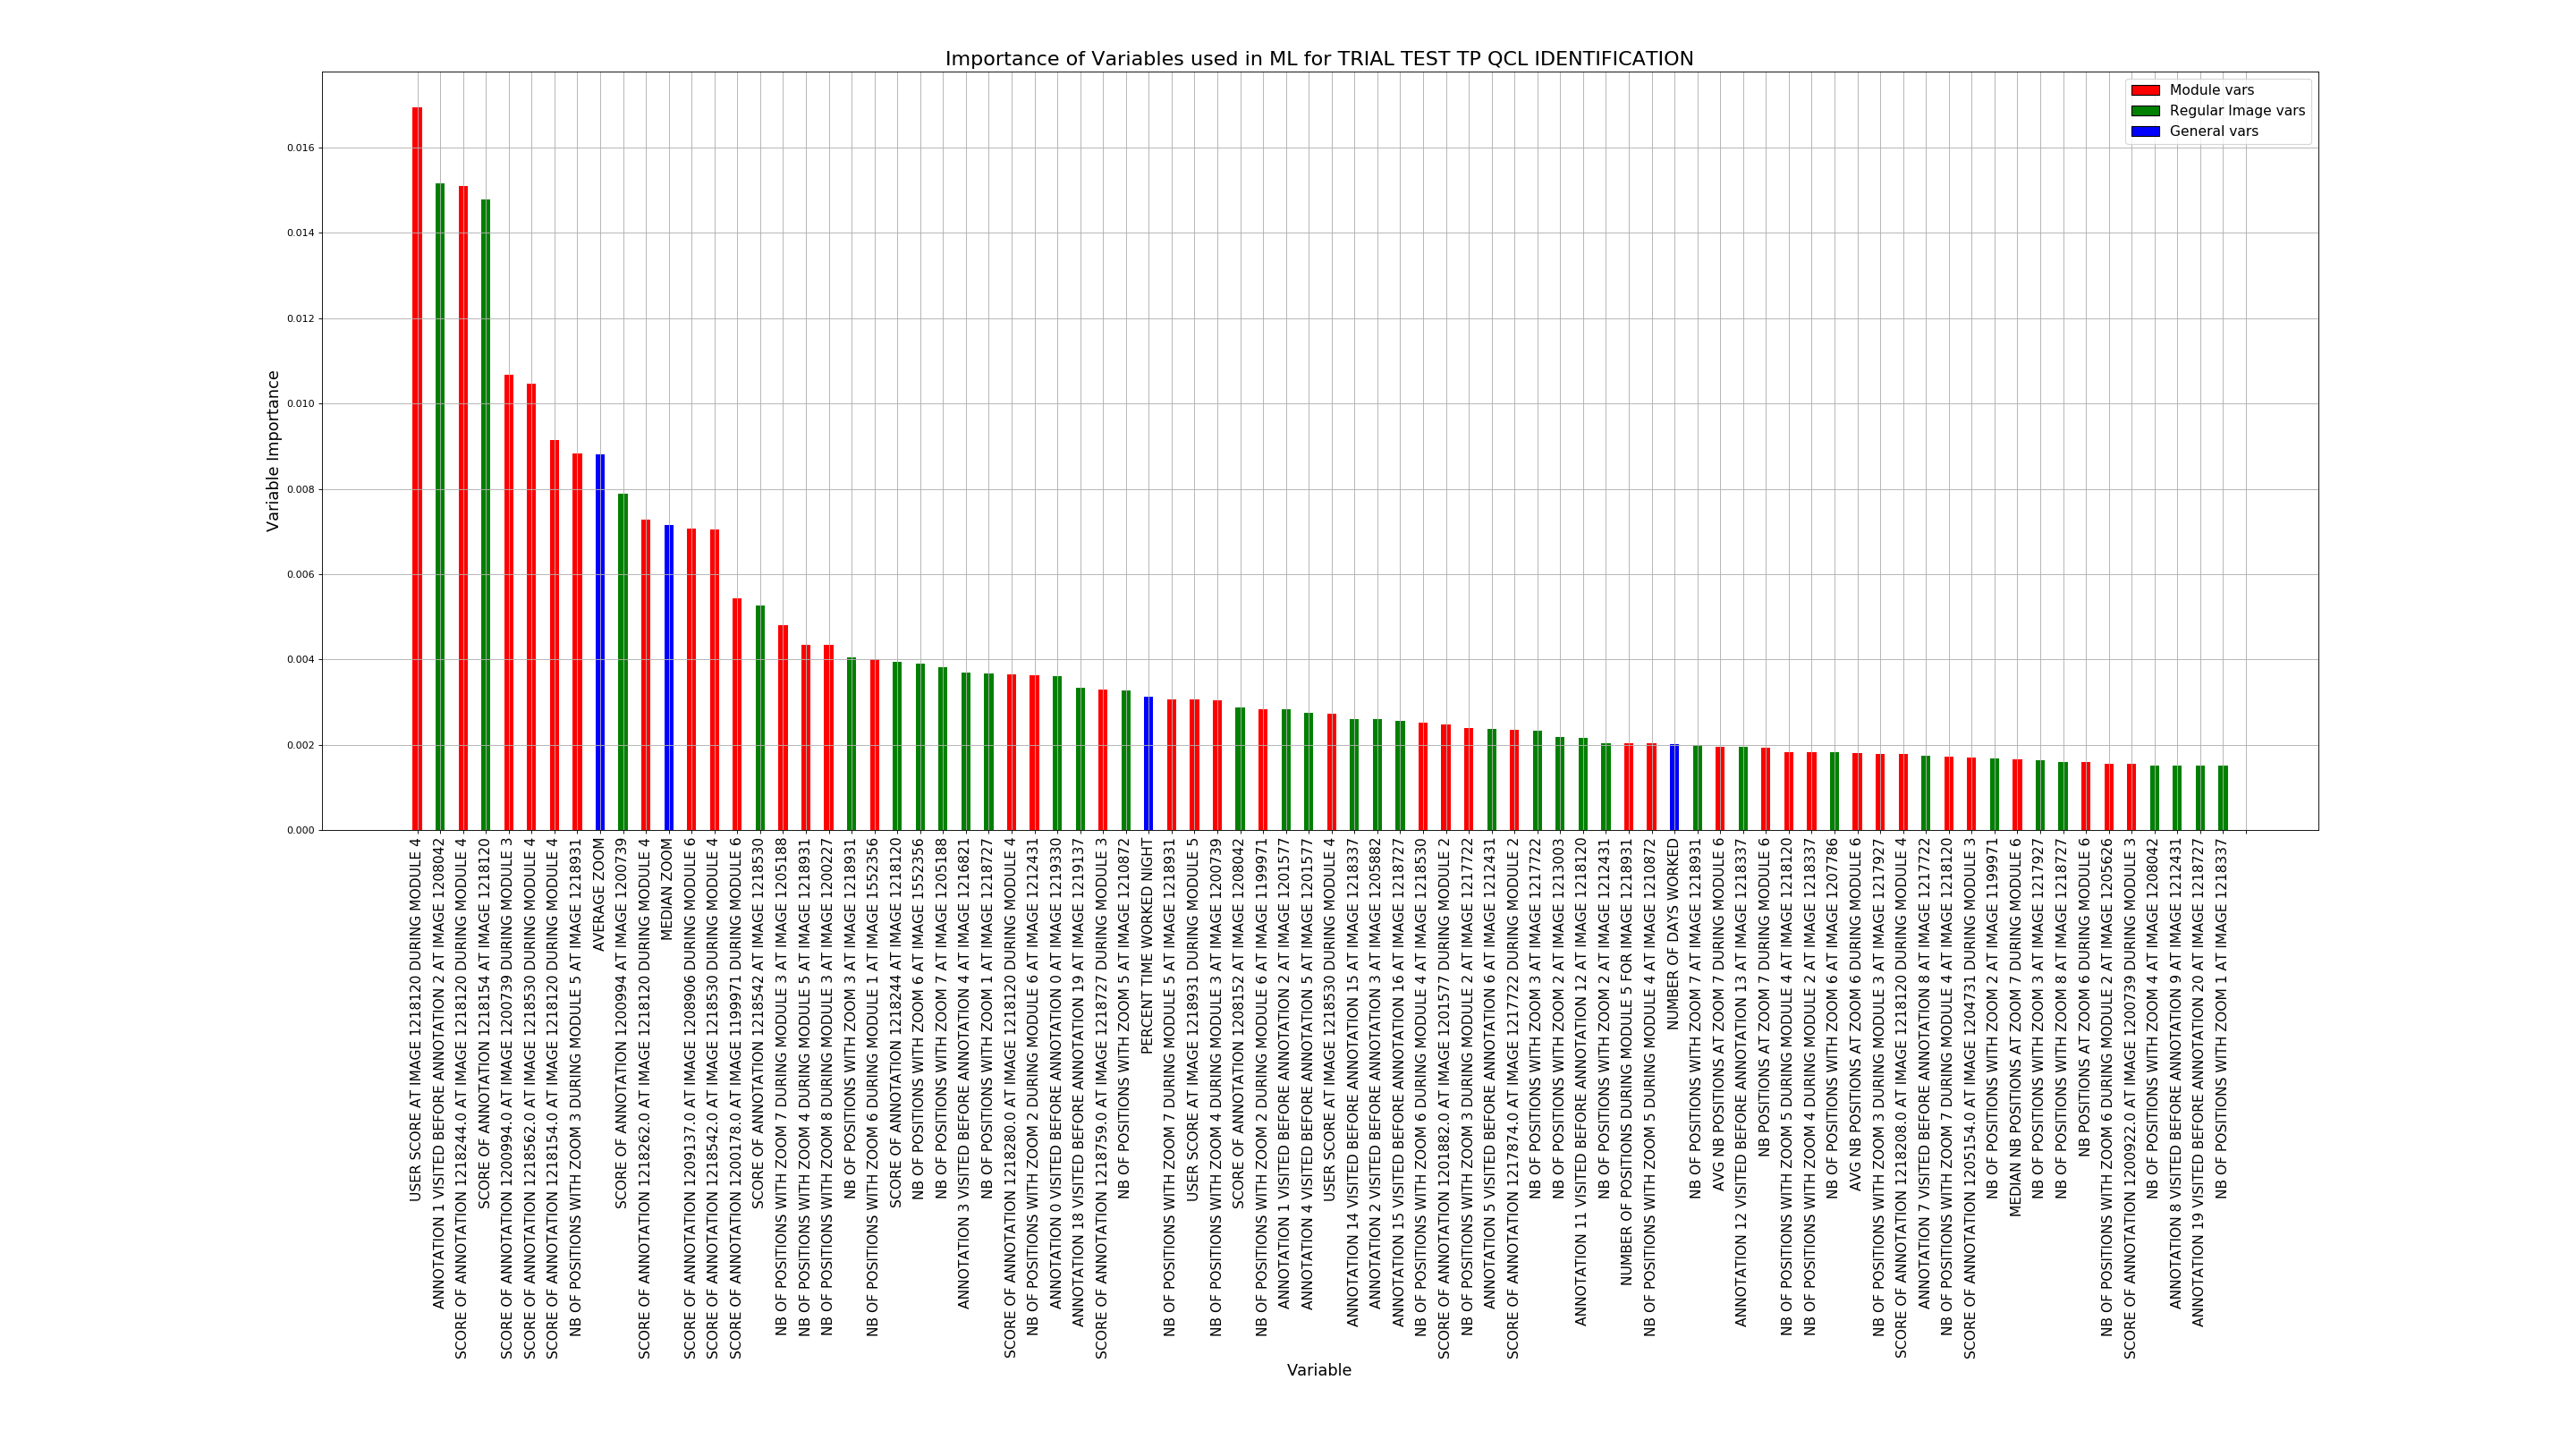
\includegraphics[width=.99\linewidth]{plots/var_importance_TRIAL_TEST_TP_QCL_IDENTIFICATION_2018-04-29_14_28_02.png}
      \caption{Feature Importance for QCL the Identification}
      \label{fig:var_white2}
      \end{figure}

      \begin{figure}[H]
      \centering
      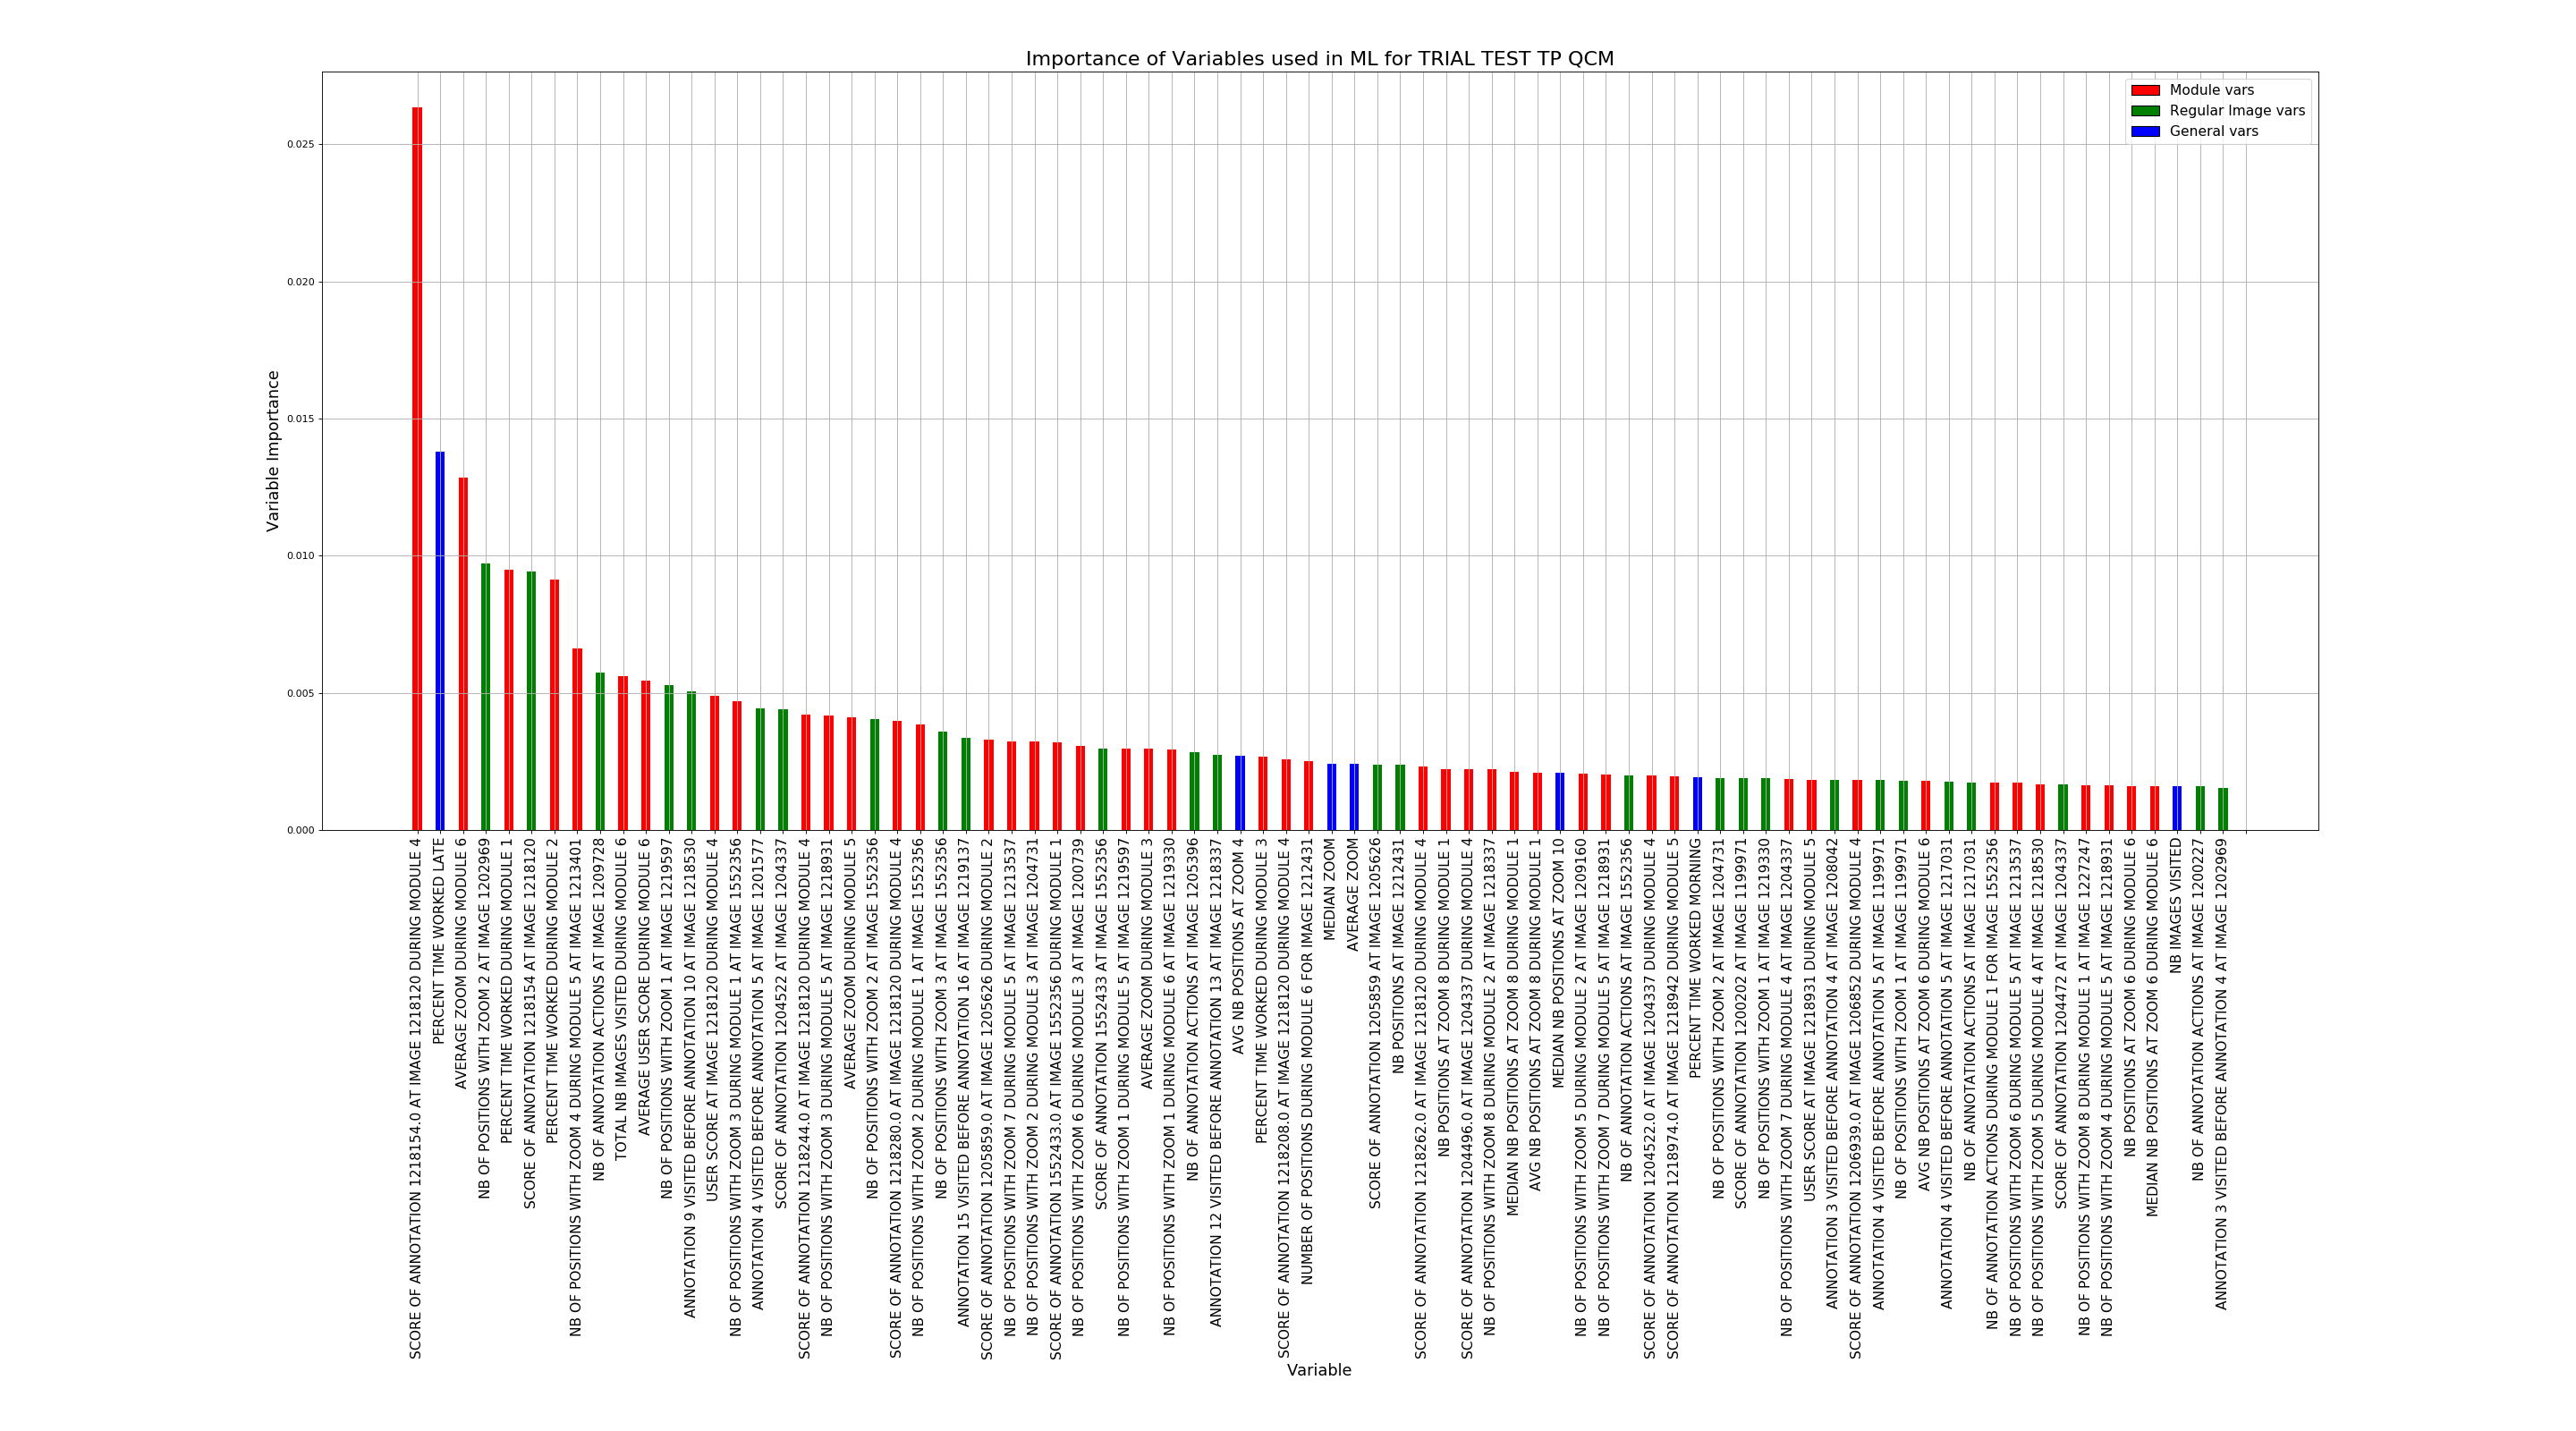
\includegraphics[width=.99\linewidth]{plots/var_importance_TRIAL_TEST_TP_QCM_2018-04-29_14_34_16.png}
      \caption{Feature Importance for the QCM}
      \label{fig:var_white3}
      \end{figure}

    These figures show the top 80 features (or \textbf{X} variable) for their respective model.
    Even though each model shares the same features, their importance varies model to model.
    But it is probable that some features from a specific image can be at the top for multiple model.
    Anyways, features are split into 3 categories:
    \begin{itemize}
    \item[\textbullet] \textbf{General Features :} Features that describes the data on the set of images as a whole. (average, median, etc..)
    \item[\textbullet] \textbf{Regular Image Features :} Features that describe the data on a specific image. (number of positions at image XXXX)
    \item[\textbullet] \textbf{Module Image Features :} Features similar to the two previous but associated to a specific module period. (number of positions at image XXXX during module Y)
    \end{itemize}

    Note that there are fewer general features, but many of those tend to have a higher importance than other image specific features.
    Apart from the incidence test, it is appropriate to say that the module variables are the most impactful.
    This is because the white exam is taken in April instead of June.
    Therefore, user performance during specific modules are better indications on the performance during the white test.
    Also, for the  identification test, the most impactful variable has a much higher importance than the rest.
    Even though this may look random, this variable may well be a good splitting factor.
    Unfortunately, this does not show the overall impact of certain images. (Figures \ref{fig:im_white1}, \ref{fig:im_white2}, \ref{fig:im_white3})

      \begin{figure}[H]
      \centering
      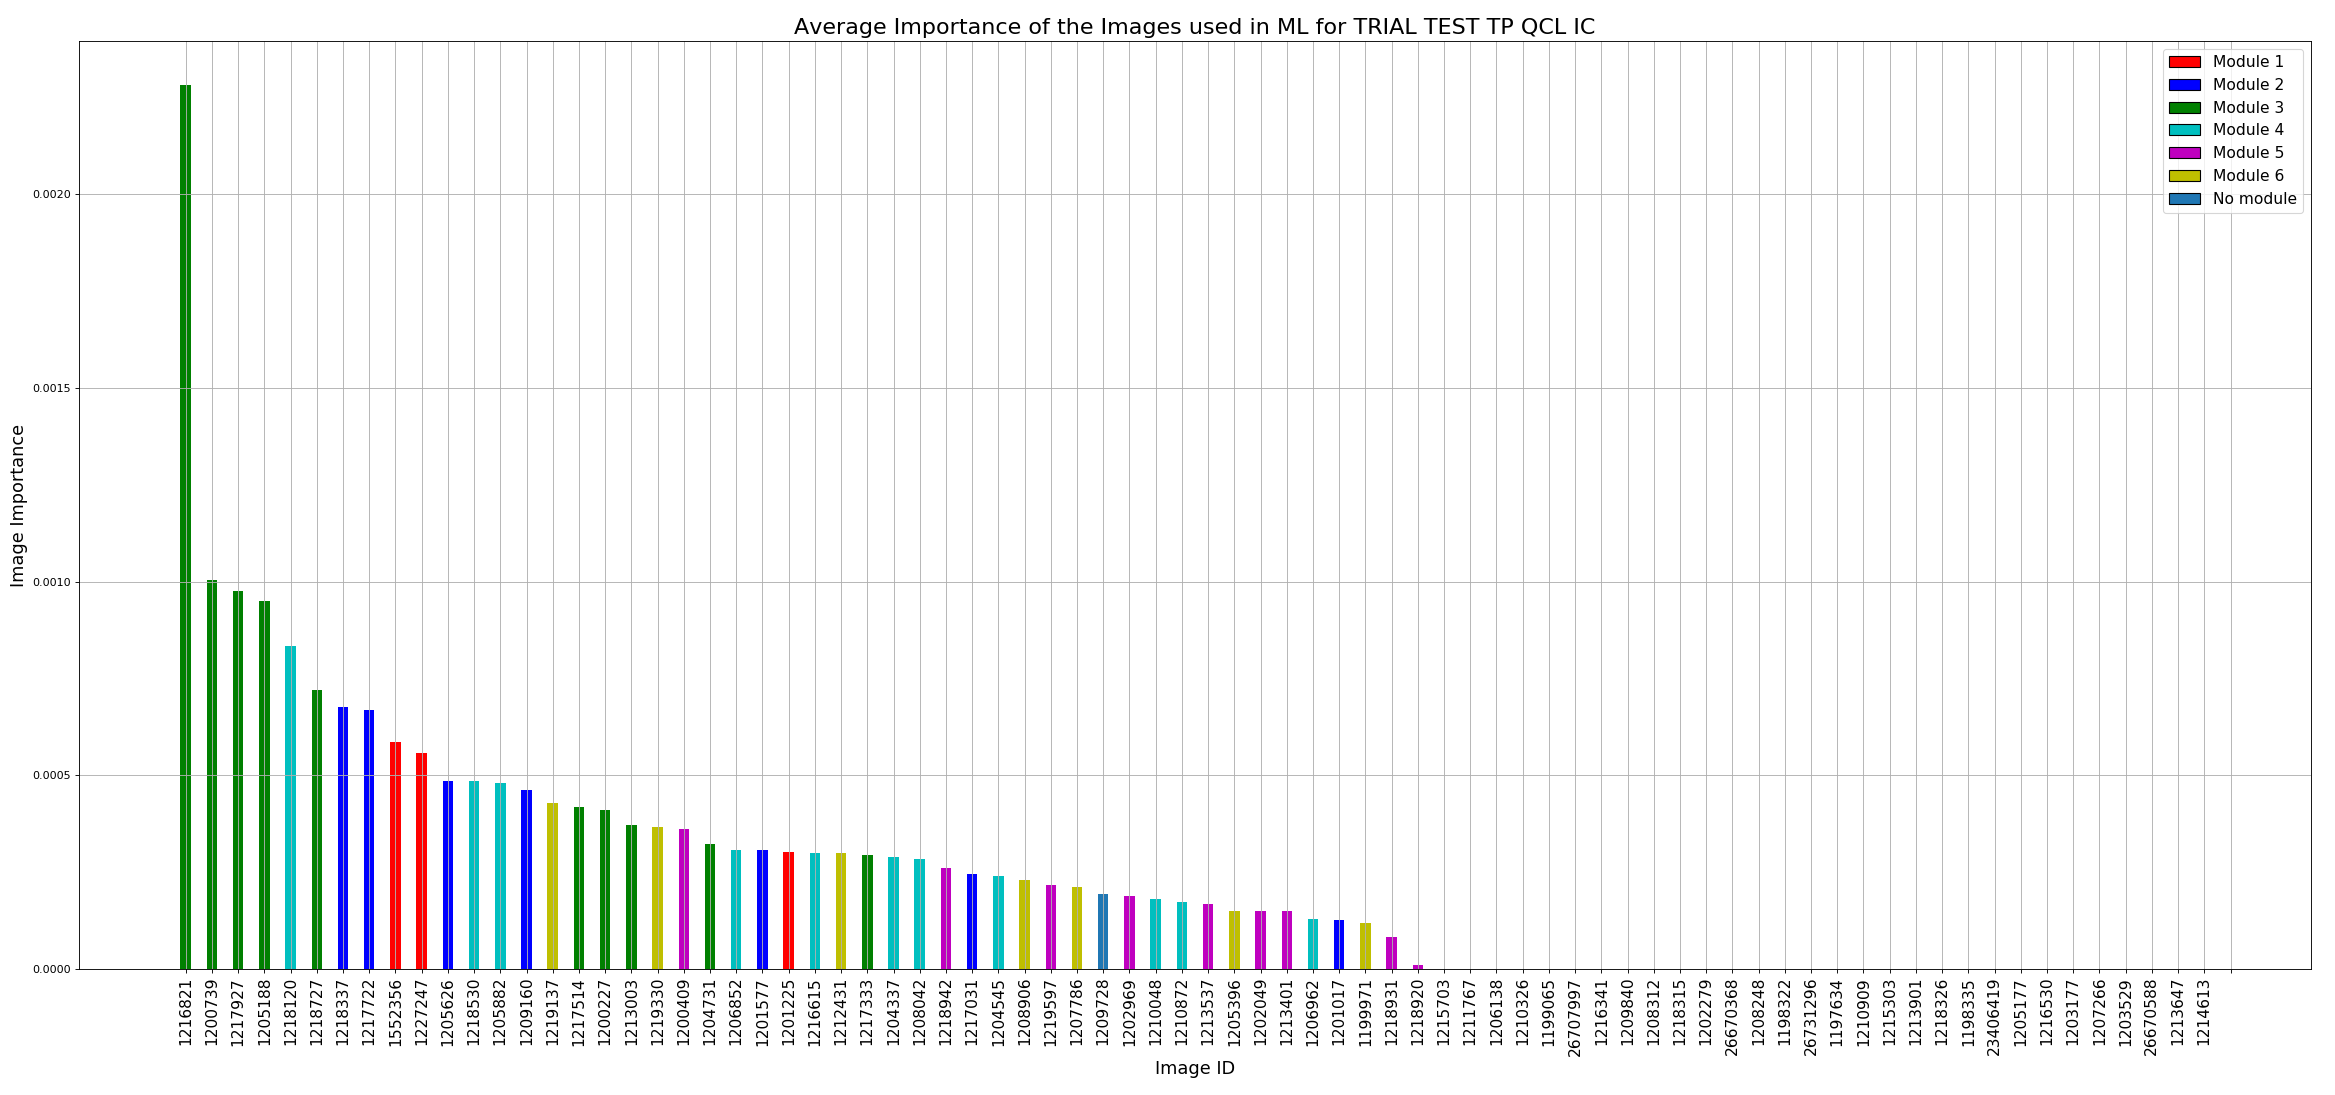
\includegraphics[width=.99\linewidth]{plots/im_importance_TRIAL_TEST_TP_QCL_IC_2018-04-29_14_31_20.png}
      \caption{Image Importance for QCL the Incidence}
      \label{fig:im_white1}
      \end{figure}

      \begin{figure}[H]
      \centering
      \includegraphics[width=.99\linewidth]{plots/im_importance_TRIAL_TEST_TP_QCL_IDENTIFICATION_2018-04-29_14_28_06.png}
      \caption{Image Importance for the QCL Identification}
      \label{fig:im_white2}
      \end{figure}

      \begin{figure}[H]
      \centering
      \includegraphics[width=.99\linewidth]{plots/im_importance_TRIAL_TEST_TP_QCM_2018-04-29_14_34_19.png}
      \caption{Image Importance for the QCM}
      \label{fig:im_white3}
      \end{figure}

    As a reminder, out of all the images in the GOLD project, about a third of the images were not even visited.
    Also, some of the images don't belong to any module.
    It seems that as a general consensus that the most impactful images often do not belong to the last module.
    This is because that the module 6 is not included in the trial exam.
    It is also worth noting that the module 1 is not included in the exam either.
    But since the module 1 is considered a tutorial, it can be useful.
    An image that appears often at the top is the image 1218120.
    This image was used for a preparation identification exercise.
    It seems that those who perform better in regards to that image on Cytomine do better in the white tests.
    For the QCL identification, the exercise images are often the most important over all the images in the same module.
    This seems to prove that doing the exercises seriously and correctly can lead to better grades.
    For the QCM, the image 1552356 which is a module 1 tutorial image is the most impactful alongside 1218120.
    Those who follow the tutorial may have an easier time understanding the course from the start and may perform better for the QCM. As for the incidence test, the module 3 variables seem to be the most impactful.
    This module may contain examples that allow the student to better differentiate different incidence angles for specific objects in the images.
    OF course the cross validation results are not the best, so these assumption are not necessary correct. This leads to the actual practical exam.

    \subsection{Practical Exam Grades}

	There are a total of 5 practical exam results including the total.
	These \textbf{Y} variables tested similarly to the white tests.
	The exam took place on the 12th of June 2017.
	Unlike the white exam, the students should have finished working on all the modules.
	These exams also depend on the entirety of the program unlike
the white tests.
Since these exams are graded, students should have the motivation to study and apply themselves. (Figure \ref{fig:results_prac})

    \begin{figure}[H]
      \centering
      \includegraphics[width=.30\linewidth]{plots/cv_boxplot_QCM_PRACTICAL_2018-04-27_19_12_27.png}
      \includegraphics[width=.30\linewidth]{plots/cv_boxplot_QROL_PRACTICAL_2018-04-27_19_11_08.png}\\
      \includegraphics[width=.30\linewidth]{plots/cv_boxplot_PRACTICAL_QCL_IDENTIFICATION_2018-04-27_16_59_01.png}
  	  \includegraphics[width=.30\linewidth]{plots/cv_boxplot_PRACTICAL_QCL_2018-04-27_17_10_02.png}
      \\
      \ref{fig:results_prac}.1: Boxplots of the error values
      \\
      \vspace{0.5cm}
      \begin{tabular}{| l | c | c | c | c | c |}
      \hline
      & \tiny{Score} & \tiny{Median Score} & \tiny{Score Difference} & \tiny{Real Median Grade} & \tiny{Median Est.
      Grade}\\ \hline
      \tiny{QCM practical} & \tiny{1.91} & \tiny{2.29} & \tiny{0.37} & \tiny{10.80} & \tiny{11.02}\\ \hline
      \tiny{QROL practical} & \tiny{3.25} & \tiny{3.64} & \tiny{0.39} & \tiny{7.93} & \tiny{8.60}\\ \hline
      \tiny{QCL identification Practical} & \tiny{2.87} & \tiny{3.36} & \tiny{0.50} & \tiny{11.0} & \tiny{11.59}\\ \hline
      \tiny{QCL incidence Practical} & \tiny{2.21} & \tiny{2.83} & \tiny{0.61} & \tiny{15.3} & \tiny{15.30}\\
      \hline
      \end{tabular}\\
      \vspace{0.5cm}
      \ref{fig:results_prac}.2: Discrete Results\\
      \vspace{0.3cm}
      \includegraphics[width=.30\linewidth]{plots/cv_comp_QCM_PRACTICAL_2018-04-27_19_12_27.png}
      \includegraphics[width=.30\linewidth]{plots/cv_comp_QROL_PRACTICAL_2018-04-27_19_11_08.png}\\
      \includegraphics[width=.30\linewidth]{plots/cv_comp_PRACTICAL_QCL_IDENTIFICATION_2018-04-27_16_59_01.png}
  	  \includegraphics[width=.30\linewidth]{plots/cv_comp_PRACTICAL_QCL_2018-04-27_17_10_02.png}
      \\
      \ref{fig:results_prac}.3: Actual grades compared to Predicated grades
      \caption{Results from cross-validation of the White Tests}
      \label{fig:results_prac}
    \end{figure}

	the results obtained are more interesting.
	The results vary heavily depending on the exams that were taken.
	All the scores are significantly better than their respective median compared to the trial tests.
    \begin{itemize}
    \item[\textbullet]  \textbf{QCM practical :} The best score, the boxplots show the most well rounded results.
    The 75 percentile of grades estimated have an error of less than 3 and a 25 percentile of grades with an error of less than 1.
    Unfortunately, there are still some cases with a significantly high error.
    As for relation between the expected grade and the estimated grade, there is a pattern following the red line that is stronger than other results.
    The exception being that low actual grades are overestimated by the model.
    QCM exams are usually are straight to the point.
    Students need to know the answer to question but they don't have to explain it.
    All students by definition are graded equally because the exam is straightforward and easy to correct.
    \item[\textbullet]  \textbf{QROL practical :} As opposed to the QCM, the score is significantly worse.
    This is also shown by the boxplot where the 75 percentile is at less than 4.5. By comparing the grades, it is apparent that there are more extreme grades and their estimations are off for the most part.
    This is normal because students write long and detailed responses to the questions.
    The teachers are more critical of the students.
    They look to see if students understand the contents of the course as opposed to learning by heart.
    \item[\textbullet]  \textbf{QCL identification Practical :} With a score of 2.86, this QCL does not offer the best results.
    It follows a somewhat lessened pattern of the QROL. As this portion of the exam gives the student an exhaustive list of possible answers, it is hard to a student to guess.
    It is critical that the students knows what they observe.
    Similarly to the QROL, lack of certainty lowers the grade.
    As opposed to the QCM where uncertainty is not much of an issue due to the lack of options.
    \item[\textbullet]  \textbf{QCL incidence Practical :} the incidence score  is somewhat better.
    Apart from a couple exceptions most of the real grades have a small variance.
    This helps explain the very low 75 percentile of about 3 and the big number of erroneous cases above 6.
    Since this part of the exam is similar to a QCM but with only 3 options, it is relatively easy to answer the questions correctly.
    This explains the higher grades for most students.
    \end{itemize}

    When taking practical exams the students have images to look at.
    Certain aspects of the images need to be identified before answering the questions.
    Unfortunately with the data fetched from Cytomine, it is hard to determine whether or not the students were able to identify certain concepts when using Cytomine.
    But attempting to identify the features that are close to determining whether or not a student understood the course is a start. (Figures \ref{fig:var_tp1}, \ref{fig:var_tp2}, \ref{fig:var_tp3},\ref{fig:var_tp4})

     \begin{figure}[H]
      \centering
      \includegraphics[width=.99\linewidth]{plots/var_importance_QCM_PRACTICAL_2018-04-29_14_38_13.png}
      \caption{Feature Importance for the QCM Practical}
      \label{fig:var_tp1}
      \end{figure}

      \begin{figure}[H]
      \centering
      \includegraphics[width=.99\linewidth]{plots/var_importance_QROL_PRACTICAL_2018-04-29_14_37_04.png}
      \caption{Feature Importance for the QROL Practical}
      \label{fig:var_tp2}
      \end{figure}

      \begin{figure}[H]
      \centering
      \includegraphics[width=.99\linewidth]{plots/var_importance_PRACTICAL_QCL_IDENTIFICATION_2018-04-29_14_34_11.png}
      \caption{Feature Importance for the QCL Identification}
      \label{fig:var_tp3}
      \end{figure}

      \begin{figure}[H]
      \centering
      \includegraphics[width=.99\linewidth]{plots/var_importance_PRACTICAL_QCL_2018-04-29_14_33_44.png}
      \caption{Feature Importance for the QCL Incidence}
      \label{fig:var_tp4}
      \end{figure}

The results are different from the trial tests.
For one, the Module features are relatively less impactful than before.
This shows that the total work done throughout the semester is more important than working more during specific modules.
It also is shown that the students spent the most time on Cytomine the day before the exam (see Figure \ref{fig:timelapse}).
Similar to the white tests models, the Average Score feature always shows up as an important feature.
This variable seems to be the closest variable into determining whether or not a student understands the course but it is still not perfect.
In the end, some images and some modules have more impact than others.  (Figures \ref{fig:im_tp1}, \ref{fig:im_tp2}, \ref{fig:im_tp3},\ref{fig:im_tp4})

     \begin{figure}[H]
      \centering
      \includegraphics[width=.99\linewidth]{plots/im_importance_QCM_PRACTICAL_2018-04-29_14_38_16.png}
      \caption{Image Importance for the QCM Practical}
      \label{fig:im_tp1}
      \end{figure}

      \begin{figure}[H]
      \centering
      \includegraphics[width=.99\linewidth]{plots/im_importance_QROL_PRACTICAL_2018-04-29_14_37_07.png}
      \caption{Image Importance for the QROL Practical}
      \label{fig:im_tp2}
      \end{figure}

      \begin{figure}[H]
      \centering
      \includegraphics[width=.99\linewidth]{plots/im_importance_PRACTICAL_QCL_IDENTIFICATION_2018-04-29_14_34_14.png}
      \caption{Image Importance for the QCL Identification}
      \label{fig:im_tp3}
      \end{figure}

      \begin{figure}[H]
      \centering
      \includegraphics[width=.99\linewidth]{plots/im_importance_PRACTICAL_QCL_2018-04-29_14_33_48.png}
      \caption{Image Importance for the QCL Incidence}
      \label{fig:im_tp4}
      \end{figure}

	It is hard to determine which modules were are more impactful as a whole.
    It seems that each module has at least one image that has a good impact on the result for each test.
	Like before, most these images are the ones dedicated to exercises.
	This supports the hypothesis that doing the exercises has a positive impact on the grades.
	But for example the image 1218120 does not appear at the top anymore.
    For both QCL exams, the 1219597 image has an overall big impact on the results.
	This shows that even though the models follow the same patterns, it is still varies based on the contents of the exam.\\

    Sometimes it is interesting  to look for correlations between the expected result and some features.
    This helps to see its direct impact in estimating a grade.
    In fact, with most of the the features, a higher value should mean a better score.
    To test this, the Pearson Correlation was calculated for the top 6 features of the Practical QCM. (Figure \ref{fig:corr_tp})
      \begin{figure}[H]
      \centering
      \includegraphics[width=.99\linewidth]{plots/var_correlation_QCM_PRACTICAL_2018-04-29_14_38_14.png}
      \caption{Pearson Correlation}
      \label{fig:corr_tp}
      \end{figure}

   Most of these features are score features which in short tells the model how well the user viewed the image in regards to the annotations.
   Therefore a higher value means a better observation of all the annotations.
   This correlation means that the more time the student is focused on annotations, the more likely that student is to get a better grade.
   This could explain the somewhat good Pearson Correlation for these variables.\\

   After studying the results for the practical exams, a question that can be asked is whether or not this analysis can work on Theoretical Exam grades.

    \subsection{Theoretical Exam Grades}

        The same tests were launched for the theoretical grade results.
        The main difference for the theory portion is that there are no QCL tests and two QROL tests.
        The learning done on the QROL test results of the practical showed the worst results.
        Meanwhile the QCM provided the best results.
        This trend is likely to continue. (Figure \ref{fig:results_theo})

      \begin{figure}[H]
      \centering
      \includegraphics[width=.30\linewidth]{plots/cv_boxplot_QCM_THEORY_2018-04-30_13_57_05.png}
      \includegraphics[width=.30\linewidth]{plots/cv_boxplot_QROL1_THEORY_2018-04-30_13_40_50.png}
      \includegraphics[width=.30\linewidth]{plots/cv_boxplot_QROL2_THEORY_2018-04-30_13_12_52.png}
      \\
      \ref{fig:results_theo}.1: Boxplots of the error values
      \\
      \vspace{0.5cm}
      \begin{tabular}{| l | c | c | c | c | c |}
      \hline
      & \tiny{Score} & \tiny{Median Score} & \tiny{Score Difference} & \tiny{Real Median Grade} & \tiny{Median Est.
      Grade}\\ \hline
      \tiny{QCM Theory} & \tiny{1.84} & \tiny{2.05} & \tiny{0.20} & \tiny{10.03} & \tiny{10.17}\\ \hline
      \tiny{QROL1 Theory} & \tiny{2.99} & \tiny{3.30} & \tiny{0.31} & \tiny{10.87} & \tiny{11.00}\\ \hline
      \tiny{QROL2 Theory} & \tiny{3.19} & \tiny{3.60} & \tiny{0.42} & \tiny{13.0} & \tiny{12.65}\\
      \hline
      \end{tabular}\\
      \vspace{0.5cm}
      \ref{fig:results_theo}.2: Discrete Results\\
      \vspace{0.3cm}
      \includegraphics[width=.30\linewidth]{plots/cv_comp_QCM_THEORY_2018-04-30_13_57_05.png}
      \includegraphics[width=.30\linewidth]{plots/cv_comp_QROL1_THEORY_2018-04-30_13_40_50.png}
  	  \includegraphics[width=.30\linewidth]{plots/cv_comp_QROL2_THEORY_2018-04-30_13_12_52.png}
      \\
      \ref{fig:results_theo}.3: Actual grades compared to Predicated grades
      \caption{Results from cross-validation of the practical tests}
      \label{fig:results_theo}
    \end{figure}

    As predicted, the QCM yielded the best scores while the QROL provided sub par scores.
    The assumptions made based off of the practical exams were correct.
    The Extra Trees has an easier time predicting QCM exams.
    But in this case, the QCM grades has a lower variance then the QROL.\\


    The following figures show the feature importance for their respective model (Figures \ref{fig:var_th1}, \ref{fig:var_th2}, and \ref{fig:var_th3}).

     \begin{figure}[H]
      \centering
      \includegraphics[width=.99\linewidth]{plots/var_importance_QCM_THEORY_2018-05-02_20_53_18.png}
      \caption{Feature Importance for the QCM Theory}
      \label{fig:var_th1}
      \end{figure}

      \begin{figure}[H]
      \centering
      \includegraphics[width=.99\linewidth]{plots/var_importance_QROL1_THEORY_2018-05-02_20_54_23.png}
      \caption{Feature Importance for the QROL1 Theory}
      \label{fig:var_th2}
      \end{figure}

      \begin{figure}[H]
      \centering
      \includegraphics[width=.99\linewidth]{plots/var_importance_QROL2_THEORY_2018-05-02_20_53_44.png}
      \caption{Feature Importance for the QROL2 Theory}
      \label{fig:var_th3}
      \end{figure}

    As usual, the scores are the most prominent features for all the theoretical exercises.
    It is interesting to note some differences with the practical exercices.
    This includes features that are associated to the time worked.
    It would not be too much of a stretch to theorize that studying with Cytomine during certain time periods, the student would assimilate more information.
    For example, when working after 2AM, the students may be more tired and they might retain less information.\\


    As for images themselves, the QROL questions are more specific so certain images may be the centerpiece. (Figures \ref{fig:im_th1}, \ref{fig:im_th2}, and \ref{fig:im_th3})

     \begin{figure}[H]
      \centering
      \includegraphics[width=.99\linewidth]{plots/im_importance_QCM_THEORY_2018-05-02_20_53_22.png}
      \caption{Image Importance for the QCM Theory}
      \label{fig:im_th1}
      \end{figure}

      \begin{figure}[H]
      \centering
      \includegraphics[width=.99\linewidth]{plots/im_importance_QROL1_THEORY_2018-05-02_20_54_25.png}
      \caption{Image Importance for the QROL1 Theory}
      \label{fig:im_th2}
      \end{figure}

      \begin{figure}[H]
      \centering
      \includegraphics[width=.99\linewidth]{plots/im_importance_QROL2_THEORY_2018-05-02_20_53_48.png}
      \caption{Image Importance for the QROL2 Theory}
      \label{fig:im_th3}
      \end{figure}

    As predicted, some images and modules are more relevant then others.
    For the QROL1, it seems that the question was associated information that the students learned from the modules 5 and 6.
    The image 1208906 which is an image used for learning is the most important.
    This is contrasted by the QROL1 question where the more important images are associated to the earlier modules (1 and 3).
    In this case, the image 1218727 was the most impactful.
    This image was given more as an exercise image as opposed to the previous one.
    As for the QCM, the image 1208906 also stood out.
    It is possible that, there is more educational interest behind this image.
    Visually analyzing some students' performance of this image may prove interesting.
    Out of the 10 students that obtained less than a 5 out of 20 on the QROL1 theory and less than 6 out of 20 in the QCM, 6 did not even open image 1208906 with one of them signing both portions of the exam.
    The other 4 did scan through the image and it is shown in figure \ref{fig:students1}.

    \begin{figure}[H]
      \centering

      \includegraphics[width=.30\linewidth]{images/2244448_heatmap.png}
      \includegraphics[width=.30\linewidth]{images/2244448_scanpath.png}
      \includegraphics[width=.30\linewidth]{images/2244448_points.png} \\

      \includegraphics[width=.30\linewidth]{images/2456991_heatmap.png}
      \includegraphics[width=.30\linewidth]{images/2456991_scanpath.png}
      \includegraphics[width=.30\linewidth]{images/2456991_points.png} \\

      \includegraphics[width=.30\linewidth]{images/2645248_heatmap.png}
      \includegraphics[width=.30\linewidth]{images/2645248_scanpath.png}
      \includegraphics[width=.30\linewidth]{images/2645248_points.png} \\

      \includegraphics[width=.30\linewidth]{images/6420595_heatmap.png}
      \includegraphics[width=.30\linewidth]{images/6420595_scanpath.png}
      \includegraphics[width=.30\linewidth]{images/6420595_points.png} \\

      \caption{Low graded student performance at Image 1208906}
      \label{fig:students1}
    \end{figure}

    As for the best graded students, there are 3 students who obtained a grade higher than 18 out of 20 for the QROL1 and higher than 15 out of 20 for the QCM.
    They all opened and scanned the image 1208906, figure \ref{fig:students2} shows their behavior.


    \begin{figure}[H]
      \centering

      \includegraphics[width=.30\linewidth]{images/1747564_heatmap.png}
      \includegraphics[width=.30\linewidth]{images/1747564_scanpath.png}
      \includegraphics[width=.30\linewidth]{images/1747564_points.png} \\

      \includegraphics[width=.30\linewidth]{images/1793969_heatmap.png}
      \includegraphics[width=.30\linewidth]{images/1793969_scanpath.png}
      \includegraphics[width=.30\linewidth]{images/1793969_points.png} \\

      \includegraphics[width=.30\linewidth]{images/1942114_heatmap.png}
      \includegraphics[width=.30\linewidth]{images/1942114_scanpath.png}
      \includegraphics[width=.30\linewidth]{images/1942114_points.png} \\


      \caption{High graded student performance at Image 1208906}
      \label{fig:students2}
    \end{figure}

    For some students, the scan paths do a poor job showing the pattern since the students go back and forth through annotations.
    Otherwise, there does not seem to be some specific pattern that differentiates the students with low grades to the students with high grades by looking at these images.
    The main observation that could be made is that for the high grade students is that they are either more efficient or curious.
    By efficient, it means that they do not have many positions and they are mostly located near annotations.
    They probably understood the concepts directly after opening the image once and they never opened it again.
    As for curious, the student would often visit regions  that are not annotated.
    They would spend more time viewing to see if they can learn more than just what's described by the annotations.
    Some low graded students follow this efficient pattern but to a lesser degree.
    It's hard to determine if the student understood the theory behind the image by just looking at these figures.
    However for the one low graded student (the 3rd),  it seems that the person struggled.
    The back and forth and the fact that the student has a significant higher number of positions could mean uncertainty.
    In the end, this image may have had a big impact for the QCM and QROL1 because the content of the questions could heavily be associated to the image.

    \subsection{Global Grades}

    The next objective is to study these grades as a whole.
    This includes the total theoretical grades, the total practical grade, and the exam as a whole. (Figure \ref{fig:results_tot})


      \begin{figure}[H]
      \centering
      \includegraphics[width=.30\linewidth]{plots/cv_boxplot_TOTAL_TP_2018-04-27_19_24_46.png}
      \includegraphics[width=.30\linewidth]{plots/cv_boxplot_TOTAL_THEORY_2018-04-30_13_53_15.png}
      \includegraphics[width=.30\linewidth]{plots/cv_boxplot_GLOBAL_GRADE_2018-04-30_13_48_59.png}
      \\
      \ref{fig:results_tot}.1: Boxplots of the error values
      \\
      \vspace{0.5cm}
      \begin{tabular}{| l | c | c | c | c | c |}
      \hline
      & \tiny{Score} & \tiny{Median Score} & \tiny{Score Difference} & \tiny{Real Median Grade} & \tiny{Median Est.
      Grade}\\ \hline
      \tiny{Total Practical} & \tiny{2.13} & \tiny{2.59} & \tiny{0.46} & \tiny{10.80} & \tiny{11.03}\\ \hline
      \tiny{Total Theory} & \tiny{2.02} & \tiny{2.34} & \tiny{0.32} & \tiny{10.79} & \tiny{10.87}\\ \hline
      \tiny{Global Grade} & \tiny{1.94} & \tiny{2.37} & \tiny{0.43} & \tiny{10.72} & \tiny{10.95}\\
      \hline
      \end{tabular}\\
      \vspace{0.5cm}
      \ref{fig:results_tot}.2: Discrete Results\\
      \vspace{0.3cm}
      \includegraphics[width=.30\linewidth]{plots/cv_comp_TOTAL_TP_2018-04-27_19_24_46.png}
      \includegraphics[width=.30\linewidth]{plots/cv_comp_TOTAL_THEORY_2018-04-30_13_53_15.png}
  	  \includegraphics[width=.30\linewidth]{plots/cv_comp_GLOBAL_GRADE_2018-04-30_13_48_59.png}
      \\
      \ref{fig:results_tot}.3: Actual grades compared to Predicated grades
      \caption{Results from cross-validation of the exam results}
      \label{fig:results_tot}
    \end{figure}

    As a whole, there is a mean absolute error of about 2.
    Overall, still not the best results.
    An interesting observation is that the learning algorithm has a easier time predicting theoretical grades over practical grades.
    As using Cytomine is overall a practical activity, the fact predicting theoretical grades works just as well can possibly imply that students can retain theoretical concepts with Cytomine.\\

    Observing what behaviors lead to this grade can prove useful (Figures \ref{fig:var_tot1}, \ref{fig:var_tot2}, and \ref{fig:var_tot3}).

      \begin{figure}[H]
      \centering
      \includegraphics[width=.99\linewidth]{plots/var_importance_TOTAL_TP_2018-04-29_14_37_37.png}
      \caption{Feature Importance for the total Practical}
      \label{fig:var_tot1}
      \end{figure}

      \begin{figure}[H]
      \centering
      \includegraphics[width=.99\linewidth]{plots/var_importance_TOTAL_THEORY_2018-05-02_23_31_54.png}
      \caption{Feature Importance for the total Theory}
      \label{fig:var_tot2}
      \end{figure}

      \begin{figure}[H]
      \centering
      \includegraphics[width=.99\linewidth]{plots/var_importance_GLOBAL_GRADE_2018-05-02_20_56_11.png}
      \caption{Feature Importance for the global Grade}
      \label{fig:var_tot3}
      \end{figure}

    Overall, the most impactful features are often associated to the students' performance scores for all the models.
    This indicator that the student followed the instructions has a notable impact on the results.
    Also, module features are also much less impactful than their regular counterparts.\\

    As for the images themselves the results are shown in figures \ref{fig:im_tot1}, \ref{fig:im_tot2}, and \ref{fig:im_tot3}.

      \begin{figure}[H]
      \centering
      \includegraphics[width=.99\linewidth]{plots/im_importance_TOTAL_TP_2018-04-29_14_37_40.png}
      \caption{Image Importance for the total Practical}
      \label{fig:im_tot1}
      \end{figure}

      \begin{figure}[H]
      \centering
      \includegraphics[width=.99\linewidth]{plots/im_importance_TOTAL_THEORY_2018-05-02_23_31_57.png}
      \caption{Image Importance for the total Theory}
      \label{fig:im_tot2}
      \end{figure}

      \begin{figure}[H]
      \centering
      \includegraphics[width=.99\linewidth]{plots/im_importance_GLOBAL_GRADE_2018-05-02_20_56_13.png}
      \caption{Image Importance for the global Grade}
      \label{fig:im_tot3}
      \end{figure}

    For the most part, the important images are similar to those of all the individual tests put together.
    So as a whole, there is a sizable set of images that have a high impact on the grades predicted.
    These results give an indication on what patterns can lead a student to pass.

    \subsection{Learning with additional Information}

    A small experiment is to set the White Test grades as features and learn the Global grades.
    This extra information can prove usefull.
    The experiment is to see if those who did well on the white tests do well on the main exam.
    For those who did not participate in the trial tests, they receive a value of -1 for those features.
    The results are shown in figure \ref{fig:test1_1} \& \ref{fig:test1_2}
    \begin{itemize}
        \item[\textbullet] Score : 1.79
        \item[\textbullet] Score from Median Model : 2.37
        \item[\textbullet] Score Difference : 0.58
    \end{itemize}
      \begin{figure}[H]
      \centering
      \includegraphics[width=.40\linewidth]{plots/test1_cv_boxplot_GLOBAL_GRADE_2018-05-17_20_39_42.png}
      \includegraphics[width=.40\linewidth]{plots/test1_cv_comp_GLOBAL_GRADE_2018-05-17_20_39_42.png}\\
      \includegraphics[width=.99\linewidth]{plots/test1_var_correlation_GLOBAL_GRADE_2018-05-17_10_12_19.png}
      \caption{White Test as features : Results - Statistics}
      \label{fig:test1_1}
      \end{figure}
      \begin{figure}[H]
      \centering
      \includegraphics[width=.99\linewidth]{plots/test1_var_importance_GLOBAL_GRADE_2018-05-17_10_12_18.png}
      \caption{White Test as features : Results - Feature Importance}
      \label{fig:test1_2}
      \end{figure}
    As is clearly visible, The three white tests had an impact on the results.
    They became by far the most important features according to Figure \ref{fig:test1_2}.
    There is also a strong correlation between those features and the exam results.
    It is hypothetically possible that in general, students who do better for the white tests do better on the final exam.
    This extra information also helped predict better results as a whole.
    This explains the reason why Teachers heavily encourage students to take the white tests.
    It gives student an idea on how the exam will be like.
    They can also get feedback if they had any questions.
    Of course, the cross validation results are still far from ideal so it is still dangerous to make too many assumptions.\\

    The next experiment tries to learn practical results all while knowing the theoretical results.
    The goal the correlation between theory and practical.
    This can also help determine an ideal prediction.
    The figures \ref{fig:test2_1} and \ref{fig:test2_2} show these results.
    \begin{itemize}
        \item[\textbullet] Score : 1.56
        \item[\textbullet] Score from Median Model : 2.59
        \item[\textbullet] Score Difference : 1.03
    \end{itemize}
      \begin{figure}[H]
      \centering
      \includegraphics[width=.40\linewidth]{plots/test2_cv_boxplot_TOTAL_TP_2018-05-18_14_11_28.png}
      \includegraphics[width=.40\linewidth]{plots/test2_cv_comp_TOTAL_TP_2018-05-18_14_11_28.png}\\
      \includegraphics[width=.99\linewidth]{plots/test2_var_correlation_TOTAL_TP_2018-05-18_02_51_44.png}
      \caption{Theoretical results as features : Results - Statistics}
      \label{fig:test2_1}
      \end{figure}
      \begin{figure}[H]
      \centering
      \includegraphics[width=.95\linewidth]{plots/test2_var_importance_TOTAL_TP_2018-05-18_02_51_43.png}
      \caption{Theoretical results as features : Results - Feature Importance}
      \label{fig:test2_2}
      \end{figure}
    The scores are marginally better.
    On average those who do well on the theoretical part of the course do better on the practical part.
    It is shown with the strong correlations.
    These features are also more impactful than any seen in the previous experiments.
    But even with this extra information, the score is still somewhat lackluster.
    This shows the individualism of each student.\\

    This same experiment could be done in reverse but the results would be extremely similar.

    \subsection{RandomForest Comparison}

    For this experiment, the RandomForest will be used to compare the Global Grade results with the Extra Tree method.
    The RandomForest is a popular and powerful tree Ensemble method.
    The RandomForest is configured with the following parameters.

    \begin{itemize}
        \item[\textbullet] \textbf{Number of Estimators : 100}\\
        Represents the number randomized trees generated.
        \item[\textbullet] \textbf{Max depth : None}\\
        The max depth of the trees.
        \item[\textbullet] \textbf{Bootstrap : False}\\
        Whether or not bootstrapping was implemented.
        Bootstrapping implements sampling with replacement within the training set.
        \item[\textbullet] \textbf{Max Features : Auto ( = Number of Features)}\\
        Max number of features that can be used by the randomized tree.
        \item[\textbullet] \textbf{Max leaf Nodes : None}\\
        The maximum number of leaf nodes that be present in a tree.
        \item[\textbullet] \textbf{Minimum Impurity Decrease : 0.0}\\
        A node will be split if the impurity is less than the minimum impurity decrease value.
        Threshold for early stopping tree growth.
        \item[\textbullet] \textbf{Minimum Samples Leaf : 10}\\
        The minimum number of samples required at a leaf node.
        \item[\textbullet] \textbf{Minimum Samples split : 2}\\
        The minimum number of samples required to split an internal node.
        \item[\textbullet] \textbf{Minimum Weight Fraction Leaf : 0.0}\\
        Minimum weighted fraction of the sum total of all weights (of all input samples) required at a leaf node.
        If 0.0, samples have equal weights.
        \item[\textbullet] \textbf{Criterion : msq - Mean Square Error}\\
        The method to measure the quality of a split.
        \item[\textbullet] \textbf{Out-of-bag Score : False}\\
        Whether out-of-bag samples are used to estimate how well unseen data is fitted to a regression line.
    \end{itemize}

    The results are shown in figures \ref{fig:test3_1}, \ref{fig:test3_2}, and \ref{fig:test3_2}.
    \begin{itemize}
        \item[\textbullet] Score : 2.07
        \item[\textbullet] Score from Median Model : 2.37
        \item[\textbullet] Score Difference : 0.30
    \end{itemize}

      \begin{figure}[H]
      \centering
      \includegraphics[width=.40\linewidth]{plots/cv_boxplot_GLOBAL_GRADE_2018-05-29_01_56_26.png}
      \includegraphics[width=.40\linewidth]{plots/cv_comp_GLOBAL_GRADE_2018-05-29_01_56_26.png}
      \caption{RandomForest : Results - Statistics}
      \label{fig:test3_1}
      \end{figure}

      \begin{figure}[H]
      \centering
      \includegraphics[width=.99\linewidth]{plots/var_importance_GLOBAL_GRADE_2018-05-29_11_04_26.png}
      \caption{RandomForest : Results - Feature Importance}
      \label{fig:test3_2}
      \end{figure}

      \begin{figure}[H]
      \centering
      \includegraphics[width=.99\linewidth]{plots/im_importance_GLOBAL_GRADE_2018-05-29_11_04_29.png}
      \caption{RandomForest : Results - Image Importance}
      \label{fig:test3_3}
      \end{figure}

    For one the cross validation results are weaker than the Extra counter part with a score of 1.93.
    Secondly, module variables seem to have more of an impact for the RandomForest.
    As for image importance, it seems that the same images are often at the top in terms of importance but the values are distinct between the low ranking and high ranking images.


    In the end, ExtraTrees are more advantageous because they give the opportunity for more features to be used.
    When tweaking the parameter "Minimum Sample Leaf" Random Forest ends up not even using some features while the ExtraTree's randomness allows for the usage of many more features.
    Because analyzing features and image importance is principal, other methods that are hard to interpret like neural networks are not as ideal.
    Humans are very inconsistent, this data set contains much noise because of it.
    Methods like linear regression are very sensitive to this noise and therefore not ideal.



\chapter{Discussion} \label{Discussion}

    \section{Limitations}

        First of all, the results obtained from the Machine Learning were subpar.
        A mean Absolute error of around 2.0 out of 20 is 10\% of the range which is not great.
        The main cause of which is the small data set of 395 students.
        If it was possible to group people up based on habits and patterns, 395 students would not be enough for such study.
        It is still important to stay skeptical because every person is unique.
        Some people have a much easier time learning than others.
        In such cases, the student may not need much time to understand the concepts provided by Cytomine.
        Therefore, there there are less recorded positions and actions.
        In other case, the exact opposite.
        When on Cytomine, the analyst can't be in the person's head when using the application.
        The student can go on the website and retain nothing.
        Also, the Gaze data may not be perfectly accurate.
        Without sensors that observe the user's eye movements, it is very impractical to track Gaze data.
        In most cases, a person is usually focused on or near the center of the screen.
        It is possible that they can focus more towards a corner.
        In it is current state, corners have a lower value from the calculated Gaussian distribution.
        It is also worth to mention again that positions are still recorded even when the window is not active.
        Since this issue is not easy to resolve without losing information, it also may lead to some inaccuracies.
        It is also important to note that much information is contained in the course itself.
        The course contains numerous examples of cells and tissues that is also found on Cytomine.
        It is entirely possible that students can ignore Cytomine for the most part and just learn from the course's Syllabus.\\


        But overall it may be a good thing that the results were not so great.
        It is important to keep in mind that this study is not used to encourage students to follow the directions to the letter.
        The students should be free to work on their course the way they see fit.
        If they were to fail, it is their own problem.
        It is also important to encourage different styles and methods, and not force a particular way of thinking.
        This is why the Annotation visit order features were not very impactful.
        If those variables were more impactful and the results were better, it could have implied that visiting annotations in a specific order would be important to passing the exam.
        Overall the goal is not to try and dictate how the students work.\\


        Secondly, even with sizable number of features it still feels like it is still possible to infer new features.
        The problem is to find features that can have a real impact on the results.
        For example, it is possible to generate the same features but for each day of the semester.
        This would end up adding tens of thousands of features.
        Due to the small number of individuals, it would be hard to draw conclusion for many of these features.
        It would also be just as hard to determine whether or not students understand the course.\\

        Thirdly, Cytomine comes with tools to create and edit annotations.
        Unfortunately, in its current state annotation operations are only accessible to the project manager.
        It would be interesting for students to be able to create personal annotations.
        There could be multiple applications, including :
        \begin{itemize}
            \item[\textbullet] For exercises, students can be asked to look for certain objects in images.
            These objects can be annotated.
            These annotations can be seen by the teachers.
            After a certain deadline, teachers can correct and give advice to students.
            \item[\textbullet] For the images used for teaching, students can annotate and describe certain objects similarly to before.
            But this time, it is used to ask questions to the teachers.
            For example on Cytomine, teachers can be notified.
            Afterwards, they can reply to these questions.
            This can be a interactive way fo students to communicate with teachers.
            \item[\textbullet] Private annotations for the students, Simply to keep information on certain objects saved and easily accessible.
        \end{itemize}
        This option for students can help improve the course in the long run.

    \section{Assets}

        This tool was able to generate many ways to visually observe user behavior on Cytomine. This includes :
        \begin{itemize}
            \item[\textbullet] Gazemaps (Gaze Heatmaps)
            \item[\textbullet] Scan Paths
            \item[\textbullet] Timelines
            \item[\textbullet] Feature importance graphs
            \item[\textbullet] Image Importance graphs
            \item[\textbullet] Feature correlation graphs
            \item[\textbullet] Cross Validation error Boxplots
            \item[\textbullet] Cross Validation error Scatter Plots
        \end{itemize}

        These tools can give indication on what the students are doing and when they are doing it.
        It is unfortunate that generating some of the figures may take some time.
        But with this tool, it is possible to generate Scan Paths or Gazemaps for specific image and user pairs on demand.
        This can be directly implemented on a Cytomine website and not necessarly only for the MOOC.\\


        Even though the Machine Learning results were not the best, the variable importance can still give small indications on what can lead students to pass or fail exams.
        For example, the features that are student's performance score in regards to annotations quantifies how well a student follows instructions.
        These features often are the top in regards to importance.
        The main thing that can be determined is which annotations had the most impact for the exam.
        This leads to image importance, and which images were the most impactful.
        A good example is for the QROL1 and the QROL2, the differences are clear.
        These results could be interpreted using Gazemaps or scan paths to visually see the link with an image.
        One question was most likely more associated to the earlier portion of the course while the other was more associated to the end of the course.
        This is theorized without actually knowing the contents of the two questions.



\chapter{Conclusion}

    The goal with this study was to analyze user behavior using the new tools that Cytomine offered.
    By studying user behavior, one can learn much about the varying ways that users use the application.
    In some cases it may be possible to analyze their reasoning.
    Comparing a set of students based on the grades they obtained for their exams could give more insight on what can differentiate students.
    This could also give insight on what works well with Cytomine and what needs improvements.
    Overall, there were some interesting results.
    This tool provided the means to analyze and visualize user behavior on Cytomine.
    Gazemaps and Scan paths provide some key information on the viewing pattern for a single image while timelines gave an overview on the project as a whole.
    Machine Learning methods have been attempted and the results give much insight on groups of people but also individuals.
    The results obtained were not the best due to the lack of individuals and the fact that this study has been carried out on people who each has there own way of thinking and doing things.
    The goal was not to turn people into robots where there is only one good way of doing an activity, it is more to understand the reasoning behind decisions and why it was done.
    Of course there still is much more information that can still be extracted and there may be even more complexity associated to it.
    A background in psychology would complement the analysis in understanding the behavioral component when using Cytomine.
    Anyways this study proposes new tools that be used by Cytomine to draw statistics and even some minor adjustments to the MOOC.
    An abstract of this study has been accepted at the  ECDP (European Congress on Digital Pathology) 2018 conference and an extended abstract has been submitted.


\bibliography{main}{}
\bibliographystyle{plain}


\chapter*{Annexes}

\begin{table}[h!]
\resizebox{\textwidth}{!}{
    \begin{tabular}{|l|l|l|}
        \hline
        \textbf{Project} & \textbf{Source code (used for this project)} & \textbf{Website} \\ \hline
        Cytomine Analysis Tool & https://github.com/lvanhee42/Master-Thesis & https://cytomine.coop/\\ \hline
        Cytomine & https://github.com/cytomine & https://cytomine.coop/ \\ \hline
        PyGazeAnalyser & https://github.com/lvanhee42/PyGazeAnalyser & http://www.pygaze.org/ \\ \hline
        Cytomine Analysis Tool & hhttps://github.com/scikit-learn & http://scikit-learn.org/stable/ \\ \hline
    \end{tabular}}
    \caption{Source Code References}
\end{table}

\begin{table}[]
\centering
\label{ann:images}
%\begin{tabular}{|p{1.5cm}|p{1.5cm}|p{1cm}|p{1cm}|p{1.7cm}|p{0.5cm}|p{5cm}|}

\resizebox{\textwidth}{!}{
\begin{tabular}{|l|l|l|l|l|l|l|}
\hline
\textbf{id}       & \textbf{name}                                                                                         & \textbf{width}  & \textbf{height} & \textbf{Resolution ($\mu$m/pixel)} & \textbf{ann.} & \textbf{link}                                                          \\ \hline
26731296 & MOD4 SEQ3 Lame2 tendon UBC.tiff                                                              & 52524  & 73069  & 1000                  & 3           & http://cytomine.mooc.ulg.ac.be/\#tabs-image-1197608-26731296- \\ \hline
26707997 & MOD2 SEQ3 Lame2bis peau du doigt.tif                                                         & 22528  & 48128  & 1000                  & 9           & http://cytomine.mooc.ulg.ac.be/\#tabs-image-1197608-26707997- \\ \hline
26670588 & MOD2 SEQ3 Lame2bis peau                                                                      & 46080  & 19698  & 1000                  & 4           & http://cytomine.mooc.ulg.ac.be/\#tabs-image-1197608-26670588- \\ \hline
26670368 & MOD6 SEQ4 Lame0 ganglion UTAS.tiff                                                           & 43650  & 36727  & 1000                  & 6           & http://cytomine.mooc.ulg.ac.be/\#tabs-image-1197608-26670368- \\ \hline
23406419 & MOD2 SEQ4 Lame1bis trachee UCSF-UofMichigan.tiff                                             & 47530  & 26737  & 1000                  & 9           & http://cytomine.mooc.ulg.ac.be/\#tabs-image-1197608-23406419- \\ \hline
1552356  & Michigan106 Peau epaisse.tiff                                                                & 33792  & 30720  & 0.65                  & 5           & http://cytomine.mooc.ulg.ac.be/\#tabs-image-1197608-1552356-  \\ \hline
1227247  & MOD1 SEQ5 identification.tif                                                                 & 33792  & 30720  & 0.65                  & 0           & http://cytomine.mooc.ulg.ac.be/\#tabs-image-1197608-1227247-  \\ \hline
1219597  & MOD5 SEQ5 Lame2 coeur.tif                                                                    & 116736 & 165888 & 0.65                  & 16          & http://cytomine.mooc.ulg.ac.be/\#tabs-image-1197608-1219597-  \\ \hline
1219330  & MOD6 SEQ5 Lame1 langue.tif                                                                   & 65536  & 113664 & 0.65                  & 16          & http://cytomine.mooc.ulg.ac.be/\#tabs-image-1197608-1219330-  \\ \hline
1219137  & MOD6 SEQ5 Lame2 moelle.tif                                                                   & 65536  & 92160  & 0.65                  & 10          & http://cytomine.mooc.ulg.ac.be/\#tabs-image-1197608-1219137-  \\ \hline
1218942  & MOD5 SEQ5 Lame1 jonctionanorectale.tif                                                       & 79872  & 192512 & 0.65                  & 10          & http://cytomine.mooc.ulg.ac.be/\#tabs-image-1197608-1218942-  \\ \hline
1218931  & MOD5 SEQ6 lame2 document2                                                                    & 58368  & 38912  & 0.65                  & 0           & http://cytomine.mooc.ulg.ac.be/\#tabs-image-1197608-1218931-  \\ \hline
1218920  & MOD5 SEQ6 lame1 atrophie musculaire neurogene  maladie de werdnig - 2014-06-02 17.39.35.ndpi & 63488  & 43008  & 0.227                 & 0           & http://cytomine.mooc.ulg.ac.be/\#tabs-image-1197608-1218920-  \\ \hline
1218727  & MOD3 SEQ6 Lame2 jonctiongastrooesophagienne.tif                                              & 55296  & 76800  & 0.65                  & 10          & http://cytomine.mooc.ulg.ac.be/\#tabs-image-1197608-1218727-  \\ \hline
1218530  & MOD4 SEQ7 Lame1 trachee.tif                                                                  & 46080  & 80896  & 0.65                  & 10          & http://cytomine.mooc.ulg.ac.be/\#tabs-image-1197608-1218530-  \\ \hline
1218337  & MOD2 SEQ5 Lame2 jonctiongastrointestinale.tif                                                & 55296  & 136192 & 0.65                  & 10          & http://cytomine.mooc.ulg.ac.be/\#tabs-image-1197608-1218337-  \\ \hline
1218326  & Image 23.tif                                                                                 & 55296  & 136192 & 0.65                  & 0           & http://cytomine.mooc.ulg.ac.be/\#tabs-image-1197608-1218326-  \\ \hline
1218315  & Image 130.tif                                                                                & 46080  & 80896  & 0.65                  & 0           & http://cytomine.mooc.ulg.ac.be/\#tabs-image-1197608-1218315-  \\ \hline
1218120  & MOD4 SEQ7 Lame2 levre.tif                                                                    & 71680  & 95232  & 0.65                  & 10          & http://cytomine.mooc.ulg.ac.be/\#tabs-image-1197608-1218120-  \\ \hline
1217927  & MOD3 SEQ6 Lame1 levre.tif                                                                    & 71680  & 95232  & 0.65                  & 10          & http://cytomine.mooc.ulg.ac.be/\#tabs-image-1197608-1217927-  \\ \hline
1217722  & MOD2 SEQ5 Lame1 levre.tif                                                                    & 71680  & 95232  & 0.65                  & 10          & http://cytomine.mooc.ulg.ac.be/\#tabs-image-1197608-1217722-  \\ \hline
1217514  & MOD3 SEQ3 Lame1 fundus                                                                       & 66560  & 87040  & 0.65                  & 8           & http://cytomine.mooc.ulg.ac.be/\#tabs-image-1197608-1217514-  \\ \hline
1217333  & MOD3 SEQ5 glde mammaire1.tif                                                                 & 73728  & 64512  & 0.65                  & 7           & http://cytomine.mooc.ulg.ac.be/\#tabs-image-1197608-1217333-  \\ \hline
1217031  & MOD2 SEQ4 Lame1 trachee                                                                      & 31744  & 59392  & 0.65                  & 12          & http://cytomine.mooc.ulg.ac.be/\#tabs-image-1197608-1217031-  \\ \hline
1216821  & MOD3 SEQ5 glde mammaire2.tif                                                                 & 40960  & 48128  & 0.65                  & 8           & http://cytomine.mooc.ulg.ac.be/\#tabs-image-1197608-1216821-  \\ \hline
1216615  & MOD4 SEQ4 Lame1 hypoderme                                                                    & 52224  & 62464  & 0.65                  & 8           & http://cytomine.mooc.ulg.ac.be/\#tabs-image-1197608-1216615-  \\ \hline
1216530  & glde mammaire1.ndpi                                                                          & 154752 & 102400 & 0.65                  & 4           & http://cytomine.mooc.ulg.ac.be/\#tabs-image-1197608-1216530-  \\ \hline
1216341  & fundus etiquettes                                                                            & 66560  & 87040  & 0.65                  & 10          & http://cytomine.mooc.ulg.ac.be/\#tabs-image-1197608-1216341-  \\ \hline
1215703  & frottis sanguin VS conjonctif.tif                                                            & 94208  & 192512 & 0.65                  & 26          & http://cytomine.mooc.ulg.ac.be/\#tabs-image-1197608-1215703-  \\ \hline
1215303  & levre picroponceau vs2.tif                                                                   & 71680  & 95232  & 0.65                  & 16          & http://cytomine.mooc.ulg.ac.be/\#tabs-image-1197608-1215303-  \\ \hline
1214613  & L\`{e}vre test appariement  conjonctif                                                           & 71680  & 95232  & 0.65                  & 30          & http://cytomine.mooc.ulg.ac.be/\#tabs-image-1197608-1214613-  \\ \hline
1213901  & jonction test appariement conjonctif                                                         & 55296  & 136192 & 0.65                  & 32          & http://cytomine.mooc.ulg.ac.be/\#tabs-image-1197608-1213901-  \\ \hline
1213647  & estomac HE V2 (parcours muscles)                                                             & 66560  & 97280  & 0.65                  & 10          & http://cytomine.mooc.ulg.ac.be/\#tabs-image-1197608-1213647-  \\ \hline
1213537  & MOD5 SEQ3 Lame2 coeur                                                                        & 46080  & 78848  & 0.65                  & 4           & http://cytomine.mooc.ulg.ac.be/\#tabs-image-1197608-1213537-  \\ \hline
1213401  & MOD5 SEQ4 Lame2 paupiere de boeuf                                                            & 71680  & 95232  & 0.65                  & 6           & http://cytomine.mooc.ulg.ac.be/\#tabs-image-1197608-1213401-  \\ \hline
1213003  & MOD3 SEQ4 Lame2 glde salivaires                                                              & 123904 & 177152 & 0.65                  & 16          & http://cytomine.mooc.ulg.ac.be/\#tabs-image-1197608-1213003-  \\ \hline
1212431  & MOD6 SEQ2 Lame1 moelle epiniere                                                              & 65536  & 95232  & 0.65                  & 23          & http://cytomine.mooc.ulg.ac.be/\#tabs-image-1197608-1212431-  \\ \hline
1211767  & l\`{e}vre test appariement glande                                                                & 71680  & 95232  & 0.65                  & 30          & http://cytomine.mooc.ulg.ac.be/\#tabs-image-1197608-1211767-  \\ \hline
1210909  & l\`{e}vre test appariement muscles                                                               & 71680  & 95232  & 0.65                  & 42          & http://cytomine.mooc.ulg.ac.be/\#tabs-image-1197608-1210909-  \\ \hline
1210872  & MOD4 SEQ6 Lame2 queue de rat                                                                 & 48128  & 41984  & 0.65                  & 1           & http://cytomine.mooc.ulg.ac.be/\#tabs-image-1197608-1210872-  \\ \hline
1210326  & langue module0                                                                               & 60416  & 105472 & 0.65                  & 22          & http://cytomine.mooc.ulg.ac.be/\#tabs-image-1197608-1210326-  \\ \hline
1210048  & MOD4 SEQ5 Lame1 trachee                                                                      & 25600  & 29696  & 0.65                  & 11          & http://cytomine.mooc.ulg.ac.be/\#tabs-image-1197608-1210048-  \\ \hline
1209840  & Intestin coupe longitudinale HF vs 2                                                         & 70656  & 59392  & 0.65                  & 8           & http://cytomine.mooc.ulg.ac.be/\#tabs-image-1197608-1209840-  \\ \hline
1209728  & MOD3 SEQ2 Lame1 cel caliciforme                                                              & 48128  & 56320  & 0.65                  & 4           & http://cytomine.mooc.ulg.ac.be/\#tabs-image-1197608-1209728-  \\ \hline
1209160  & MOD2 SEQ2 Lame1 intestin grele                                                               & 33792  & 60416  & 0.65                  & 23          & http://cytomine.mooc.ulg.ac.be/\#tabs-image-1197608-1209160-  \\ \hline
1208906  & MOD6 SEQ3 Lame2 nerf                                                                         & 90112  & 72704  & 0.65                  & 10          & http://cytomine.mooc.ulg.ac.be/\#tabs-image-1197608-1208906-  \\ \hline
1208312  & jonction test appariement nerfs                                                              & 55296  & 136192 & 0.65                  & 24          & http://cytomine.mooc.ulg.ac.be/\#tabs-image-1197608-1208312-  \\ \hline
1208248  & paquet vasculo nerveux orc\'{e}ine vs 2                                                          & 30720  & 29696  & 0.65                  & 2           & http://cytomine.mooc.ulg.ac.be/\#tabs-image-1197608-1208248-  \\ \hline
1208042  & MOD4 SEQ2 Lame4 oesophage                                                                    & 62464  & 57344  & 0.65                  & 8           & http://cytomine.mooc.ulg.ac.be/\#tabs-image-1197608-1208042-  \\ \hline
1207786  & MOD6 SEQ3 Lame1 paquet vasculo-nerveux                                                       & 26624  & 23552  & 0.65                  & 10          & http://cytomine.mooc.ulg.ac.be/\#tabs-image-1197608-1207786-  \\ \hline
1207266  & Frottis de sang May Gr\"{u}nwald Giemsa VS2                                                      & 94208  & 192512 & 0.65                  & 28          & http://cytomine.mooc.ulg.ac.be/\#tabs-image-1197608-1207266-  \\ \hline
1206962  & MOD4 SEQ2 Lame1 intestin grele                                                               & 33792  & 60416  & 0.65                  & 12          & http://cytomine.mooc.ulg.ac.be/\#tabs-image-1197608-1206962-  \\ \hline
1206852  & MOD4 SEQ2 Lame3 trachee                                                                      & 25600  & 29696  & 0.65                  & 4           & http://cytomine.mooc.ulg.ac.be/\#tabs-image-1197608-1206852-  \\ \hline
1206138  & jonction test appariement epith rev                                                          & 55296  & 136192 & 0.65                  & 34          & http://cytomine.mooc.ulg.ac.be/\#tabs-image-1197608-1206138-  \\ \hline
1205882  & MOD4 SEQ6 Lame1 tibia                                                                        & 57344  & 95232  & 0.65                  & 10          & http://cytomine.mooc.ulg.ac.be/\#tabs-image-1197608-1205882-  \\ \hline
1205626  & MOD2 SEQ3 Lame1 oesophage                                                                    & 62464  & 57344  & 0.65                  & 10          & http://cytomine.mooc.ulg.ac.be/\#tabs-image-1197608-1205626-  \\ \hline
1205396  & MOD6 SEQ3 Lame3 levre                                                                        & 71680  & 95232  & 0.65                  & 9           & http://cytomine.mooc.ulg.ac.be/\#tabs-image-1197608-1205396-  \\ \hline
1205188  & MOD3 SEQ5 Lame3 glde sebacee                                                                 & 71680  & 92160  & 0.65                  & 8           & http://cytomine.mooc.ulg.ac.be/\#tabs-image-1197608-1205188-  \\ \hline
1205177  & Lame d intestin gr\^{e}le.tif                                                                    & 72704  & 80896  & 0.65                  & 0           & http://cytomine.mooc.ulg.ac.be/\#tabs-image-1197608-1205177-  \\ \hline
1204731  & MOD3 SEQ4 Lame1 pancreas                                                                     & 72704  & 72704  & 0.65                  & 18          & http://cytomine.mooc.ulg.ac.be/\#tabs-image-1197608-1204731-  \\ \hline
1204545  & MOD4 SEQ3 Lame1 tendon                                                                       & 48128  & 41984  & 0.65                  & 6           & http://cytomine.mooc.ulg.ac.be/\#tabs-image-1197608-1204545-  \\ \hline
1204337  & MOD4 SEQ2 Lame2 peau                                                                         & 52224  & 62464  & 0.65                  & 8           & http://cytomine.mooc.ulg.ac.be/\#tabs-image-1197608-1204337-  \\ \hline
1203529  & trach\'{e}e test appariement muscles                                                             & 46080  & 80896  & 0.65                  & 38          & http://cytomine.mooc.ulg.ac.be/\#tabs-image-1197608-1203529-  \\ \hline
1203177  & trach\'{e}e coupe longitudinale bleu alcian nuclear fast red VS2                                 & 28672  & 38912  & 0.65                  & 14          & http://cytomine.mooc.ulg.ac.be/\#tabs-image-1197608-1203177-  \\ \hline
1202969  & MOD5 SEQ4 Lame1 intestin grele                                                               & 72704  & 80896  & 0.65                  & 9           & http://cytomine.mooc.ulg.ac.be/\#tabs-image-1197608-1202969-  \\ \hline
1202279  & trachee test appariement nerfs                                                               & 46080  & 80896  & 0.65                  & 30          & http://cytomine.mooc.ulg.ac.be/\#tabs-image-1197608-1202279-  \\ \hline
1202049  & MOD5 SEQ3 Lame1 myocarde                                                                     & 44032  & 61440  & 0.65                  & 9           & http://cytomine.mooc.ulg.ac.be/\#tabs-image-1197608-1202049-  \\ \hline
1201577  & MOD2 SEQ3 Lame2 peau du doigt                                                                & 31744  & 38912  & 0.65                  & 19          & http://cytomine.mooc.ulg.ac.be/\#tabs-image-1197608-1201577-  \\ \hline
1201225  & MOD1 SEQ5 Parcours guid\'{e}                                                                     & 60416  & 105472 & 0.65                  & 14          & http://cytomine.mooc.ulg.ac.be/\#tabs-image-1197608-1201225-  \\ \hline
1201017  & MOD2 SEQ3 Lame3 paupiere                                                                     & 69632  & 70656  & 0.65                  & 8           & http://cytomine.mooc.ulg.ac.be/\#tabs-image-1197608-1201017-  \\ \hline
1200739  & MOD3 SEQ3 Lame2 glde sud eccrine                                                             & 52224  & 62464  & 0.65                  & 11          & http://cytomine.mooc.ulg.ac.be/\#tabs-image-1197608-1200739-  \\ \hline
1200409  & MOD5 SEQ2 Lame1 langue de lapin                                                              & 80896  & 94208  & 0.65                  & 13          & http://cytomine.mooc.ulg.ac.be/\#tabs-image-1197608-1200409-  \\ \hline
1200227  & MOD3 SEQ2 Lame2 epit muci gastrique                                                          & 66560  & 97280  & 0.65                  & 8           & http://cytomine.mooc.ulg.ac.be/\#tabs-image-1197608-1200227-  \\ \hline
1199971  & MOD6 SEQ4 Lame1 intestin grele                                                               & 38912  & 67584  & 0.65                  & 10          & http://cytomine.mooc.ulg.ac.be/\#tabs-image-1197608-1199971-  \\ \hline
1199065  & levre test appariement epith rev                                                             & 71680  & 95232  & 0.65                  & 46          & http://cytomine.mooc.ulg.ac.be/\#tabs-image-1197608-1199065-  \\ \hline
1198335  & jonction test appariement glande                                                             & 55296  & 136192 & 0.65                  & 38          & http://cytomine.mooc.ulg.ac.be/\#tabs-image-1197608-1198335-  \\ \hline
1198322  & Queue de rat HE ou safranine                                                                 & 33792  & 30720  & 0.65                  & 0           & http://cytomine.mooc.ulg.ac.be/\#tabs-image-1197608-1198322-  \\ \hline
1197634  & Moelle \'{e}pini\`{e}re VS2                                                                          & 48128  & 39936  & 0.65                  & 28          & http://cytomine.mooc.ulg.ac.be/\#tabs-image-1197608-1197634-  \\ \hline
\end{tabular}}

\caption{Images in the GOLD project}
\end{table}

\end{document}